%%%%%%%%%%%%%%%%%%%%%%%%%%%%%%%%%%%%%%%%%%%%%%%%%%%%%%%%%%%%%%%%%%%
%                                                                 %
%                            ROOT FILE                            %
%                                                                 %
%%%%%%%%%%%%%%%%%%%%%%%%%%%%%%%%%%%%%%%%%%%%%%%%%%%%%%%%%%%%%%%%%%%
%
%  Run LaTeX or pdfLaTeX on this file to produce your thesis.
%  To produce the abstract title page followed by the abstract,
%  see the file abstitle-phd.tex or abstitle-mas.tex.
%
%%%%%%%%%%%%%%%%%%%%%%%%%%%%%%%%%%%%%%%%%%%%%%%%%%%%%%%%%%%%%%%%%%%

\documentclass[chap]{thesis}

% Use the first command below if you want captions over 1 line indented. A side
% effect of this is to remove the use of bold for captions (thesis default).
% To restore bold, also include the second line below.
%\usepackage[hang]{caption}      % to indent subsequent lines of captions
%\renewcommand{\captionfont}{\bfseries} % bold caption (needed with caption
                                       % package to restore boldface.)


%\includeonly{rpichap1}  % use \includeonly to process only
                         % the file(s) listed inside the braces


% ------------------------
% You MUST attribute any previously published work (even if it's your own writing)
% Attribution of previously published work
% Use the after title and before the first sentence of the chapter
% Example: \blfootnote{This work perviously appeared as: \bibentry{mypaper2015}
\makeatletter
\def\blfootnote{\xdef\@thefnmark{}\@footnotetext}
\makeatother
\usepackage{graphicx}
\usepackage{adjustbox}
\usepackage{listings}
\usepackage{textcomp}
\usepackage{tabularx}
\usepackage{tikz}
\usetikzlibrary{positioning}
\usepackage{bibentry}
\usepackage{url}
%http://tex.stackexchange.com/questions/141247/how-to-deal-with-sign-in-url-when-using-hyperref-and-bibentry
\usepackage{etoolbox}
\makeatletter
\let\ORIG@BR@c@bibitem\BR@c@bibitem
\apptocmd\ORIG@BR@c@bibitem{\endgroup}{}{}
\def\BR@c@bibitem{\begingroup\catcode`\%=12 \ORIG@BR@c@bibitem}
\makeatother
\nobibliography*

% If you have an attribution before your first in-text citation, 
% you should use \nobibentry to ensure in-text citations start at [1]
\newcommand{\ignore}[1]{}
\newcommand{\nobibentry}[1]{{\let\nocite\ignore\bibentry{#1}}}
% ------------------------

\newcolumntype{L}[1]{>{\raggedright\arraybackslash}p{#1}}
\newcolumntype{C}[1]{>{\centering\arraybackslash}p{#1}}
\newcolumntype{R}[1]{>{\raggedleft\arraybackslash}p{#1}}

\lstset{
	basicstyle=\ttfamily,
	captionpos=b,
	columns=fullflexible,
	frame=single,
	breaklines=true,
	numbers=left,
	numbersep=5pt,
}

\begin{document}

%\include{rpititle-mas}   % titlepage material for Master's thesis or project
%%%%%%%%%%%%%%%%%%%%%%%%%%%%%%%%%%%%%%%%%%%%%%%%%%%%%%%%%%%%%%%%%%%
%                                                                 %
%                            TITLE PAGE                           %
%                            PhD Thesis                           %
%                                                                 %
%%%%%%%%%%%%%%%%%%%%%%%%%%%%%%%%%%%%%%%%%%%%%%%%%%%%%%%%%%%%%%%%%%%
%  This file produces the title page, copyright page (if requested)
%  and the Table of Contents, List of Figures and List of Tables.
%
%  To produce the abstract title page followed by the abstract,
%  see the template file, "abstitle-phd.tex"
%%%%%%%%%%%%%%%%%%%%%%%%%%%%%%%%%%%%%%%%%%%%%%%%%%%%%%%%%%%%%%%%%%%

% Supply information for use on title page:
%
\thesistitle{\bf Data Set Versioning through \\ Linked Data Models}
\author{Benno Lee}
\degree{Doctor of Philosophy}
\department{Computer Science} % provide your area of study here; e.g.,
%  "Mechanical Engineering", "Nuclear Engineering", "Physics", etc.

\signaturelines{4}     %max number of signature lines is 7
\thadviser{Peter Fox}
 %\cothadviser{Second Adviser} % If you have 2 thesis advisers
\memberone{Jim Hendler}
\membertwo{Deborah MacGuiness}
\memberthree{Beth Plale}
%\memberfour{Marcus Aurelius} % must change signaturelines to 5 if using this 5 members
%\memberfive{Marcus Junius Brutus} % must change signaturelines to 6 if using this 6 members
%\membersix{Nikola Tesla} % must change signaturelines to 7 if using this 7 members

\submitdate{May 2018\\(For Graduation July 2018)}
\copyrightyear{2018}   % if omitted, current year is used.

% Print titlepage and other prefatory material:
%
\titlepage
\copyrightpage         % optional
\tableofcontents
\listoftables          % required if there are tables
\listoffigures         % required if there are figures
\listoflistings   % titlepage material for PhD thesis
%%%%%%%%%%%%%%%%%%%%%%%%%%%%%%%%%%%%%%%%%%%%%%%%%%%%%%%%%%%%%%%%%%%
%                                                                 %
%                         ACKNOWLEDGEMENT                         %
%                                                                 %
%%%%%%%%%%%%%%%%%%%%%%%%%%%%%%%%%%%%%%%%%%%%%%%%%%%%%%%%%%%%%%%%%%%

\specialhead{ACKNOWLEDGMENT}

  % include for acknowledgements
%%%%%%%%%%%%%%%%%%%%%%%%%%%%%%%%%%%%%%%%%%%%%%%%%%%%%%%%%%%%%%%%%%%
%                                                                 %
%                            ABSTRACT                             %
%                                                                 %
%%%%%%%%%%%%%%%%%%%%%%%%%%%%%%%%%%%%%%%%%%%%%%%%%%%%%%%%%%%%%%%%%%%

\specialhead{ABSTRACT}

Data sets invariably require versioning systems to manage changes due to an imperfect collection environment.
While importance grows, versioning discussion remains imprecise, lacking standardization or formal specifications.
Many works tend to define versions around examples and local characteristics but lack a broader foundation.
This imprecision results in a reliance on change brackets and dot-decimal identifiers without quantitative measures to justify their application.
No difference exists between the versioning practices of a group which updates their data regularly and a group which adds many new files but rarely replaces them.
This work attempts to improve discussion by capturing version relationships into a linked data model, taking inspiration from provenance models that incorporate versioning concepts such as PROV and PAV.
The model captures addition, invalidation, and modification relationships between versions to provide change log-like characterization of the differences.
This approach demonstrated increased expressibility of change interactions, but encountered issues with space scalability.
The model's generation also revealed a four step process to conduct versioning: validation, mapping, computation, and publishing.
Quantifying these changes also provided a numerical basis for evaluating the GCMD Keywords taxonomy's adopted identification scheme.
It also demonstrates the ability of versioning methods to actively influence scientific designs through performance assessment. % abstract
%%%%%%%%%%%%%%%%%%%%%%%%%%%%%%%%%%%%%%%%%%%%%%%%%%%%%%%%%%%%%%%%%%%
%                                                                 %
%                            CHAPTER ONE                          %
%                                                                 %
%%%%%%%%%%%%%%%%%%%%%%%%%%%%%%%%%%%%%%%%%%%%%%%%%%%%%%%%%%%%%%%%%%%

\chapter{INTRODUCTION}

\section{Introduction}

\begin{quotation}
	If scientific data production were easy, instruments would
	have stable calibrations and validation activities would discover no need for
	corrections that vary with time. Unfortunately, validation invariably shows that
	instrument calibrations drift and that algorithms need a better physical basis.
\end{quotation} \cite{Barkstrom2003}.

Anyone who has used an iPhone or owned a video game console understands the basics of versioning.
Companies brand sequential devices to indicate improvements in performance or capabilities.
This basic identification method has given rise to a plethora of versioning systems used widely across a landscape of software and data.
They help scientific workflows avoid losing work by managing transitions and changes while in operation \cite{Casati1996}.
They provide necessary documentation which informs the transition to new methods and procedures \cite{Wiil:2000:RDH:338407.338517}.
They provide accountability for the value of a project's data set when considering an agency's continued funding \cite{Cavanaugh2002}.
The natural evolution of these systems, however, have given rise to formal architecture operating on top of very informal concepts.
In this dissertation, we identify gaps in versioning practices which result from tradition and develop a data model to more completely capture the interactions involved in versioning.

\section{Definitions of Version}

Using versions in the vernacular has become so pervasive that few documents formally define it.
Barkstrom describes versions as \textbf{homogeneous groupings} used to control, ``production volatility induced by changes in algorithms and coefficients as result of validation and reprocessing," \cite{Barkstrom2003}.
The \textbf{groupings} he mentions is a method of separating data objects such that they have similar scientific or technical properties.
In order to determine when these properties have changed, he leverages the NASA workflow model shown in Figure \ref{NASALevels}.
\begin{figure}
	\centering
	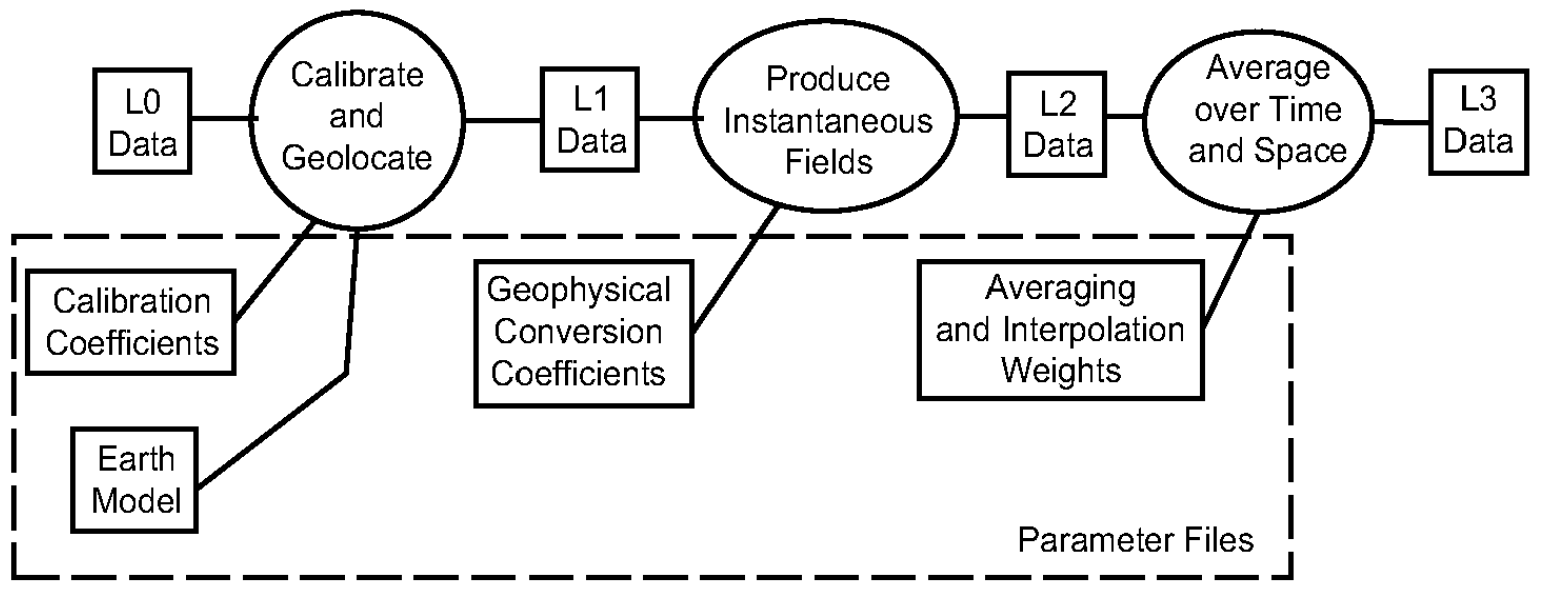
\includegraphics[scale=0.35]{figures/NASALevels.png}
	\caption[NASA organizes its data into three levels depending on the amount of aggregation and the distance the data is removed from the original sensor measurements.]{NASA organizes its data into three levels depending on the amount of aggregation and the distance the data is removed from the original sensor measurements. Figure 1 from \cite{Barkstrom2003}}
	\label{NASALevels}
\end{figure}
The model describes the formal stages of processing to turn a raw remote sensing signal from satellite instruments into global aggregate summaries \cite{Barkstrom2003}.
Understanding this model reveals that changes to either the algorithms or parameter files will force a change in the resulting data, creating a new version of the output data.
Essentially, versions are a means to communicate how much data has diverged as a result of changes to an object's provenance.

Another definition comes from Tagger in which versions are a, ``semantically meaningful snapshot of a design object," \cite{Tagger2005}.
He, unfortunately, does not further clarify what he means by semantically meaningful.
The design object unifies the versions as their primary subject, capturing the object's state over the course of its design.

The derivation, PROV Ontology's analog for a version and covered more in Section \ref{sec:prov}, is defined as, ``a transformation of an entity into another, an update of an entity resulting in a new one, or the construction of a new entity based on a pre-existing entity," \cite{Lebo2013}.
In this view, a \textbf{version} exists in comparison to another object.

The Functional Requirements for Bibliographical Records (FRBR) avoids the terms \textbf{edition} and \textbf{version} since ``those terms are neither clearly defined nor uniformly applied" \cite{frbr}.
Instead, they use the terms: work, expression, and manifestation.
A \textbf{work} refers to the abstract concept of a creative or artistic idea.
\textbf{Expressions} are then different forms of that particular \textbf{work}, embodying the most similar term to versions.
A \textbf{manifestation} is the physical embodiment of an \textbf{expression}.
These three terms and their hierarchy establish a repeating theme throughout other versioning works.
Combining these myriad of definitions together, a version is an \textbf{expression} of a \textbf{work} which exists in comparison to another object and communicates the extent to which it diverges from that object as a result of provenance changes.

\section{Version Systems} \label{sec:system}

Versioning systems take many different forms from Clotho, an application conducting versioning at the block level, to Champagne, a framework to propagate change data across multiple information systems \cite{Flouris04clotho:transparent} \cite{Systems02champagne:data}.
Each approach has a unique set of challenges to overcome.
Closer to the data collection, version systems must be flexible and responsive to adapt to changing environments, but as the socio-technical distance of a repository increases away from the collection site, more formal methods are required to unify repositories \cite{Baker2009}.
Different approaches are also necessary to account for the needs of different domains.
Versioning an XML text-file will need to account for serial file input and output as well as structured markup \cite{Chien:2000:VMX:646544.696357}.
Many applications have adopted a tree-like structure which is further propagated by software versioning managers (SVM) \cite{Stuckenholz:2005:CEV:1039174.1039197}.
The advantage being well established graph theory methods can be applied to complex objects relationships in complex environemtns \cite{Dijkstra1994}.
The growing population of web documents, however, presents a new smörgåsbord of complicated data which will need scalable solutions \cite{Berberich:2007:TMT:1277741.1277831}.

\subsection{Library Sciences}

While many of the modern systems requiring versioning managers store digital products, libraries have been tackling similar issues for a much longer time.
Libraries curate multiple editions of the same work, sometimes with significant revisions \cite{Wiil:2000:RDH:338407.338517}.
In many ways, versioned objects resemble multi-edition books or documents.
Digital librarians have faced many challenges when searching for a persistent identifier due to evolving web technologies.
Early citations referred to on-line documents using stagnant Uniform Resource Locators (URL), but this frequently lead to a condition known as link rot where moving the document would invalidate the URL \cite{Lyons2005}.
Locators required a system to manage changes of old identifiers to new locations when people attempted to utilize references from print.
The need eventually led to the development of Persistent URLs (PURL), which also suffered from link rot, and this eventually led to the distributed Digital Object Identifier (DOI) system used to track documents today \cite{Duerr2011}.
The PURL used a centralized system that would translate dead links and redirect to a document's latest location.
The system would still need to be manually updated, meaning links would rot if a document was lost or overlooked.
DOIs rely on a network of managing agencies to collect and host submitted documents.
In the specialized Handle system, the network has member agencies internally assign an unique name and concatenate it to the end of their host name.
In Figure \ref{table:Duerr}, DOIs represent the most suitable identifier used for citation in scholarly literature \cite{Duerr2011}.
\begin{figure}
	\centering
	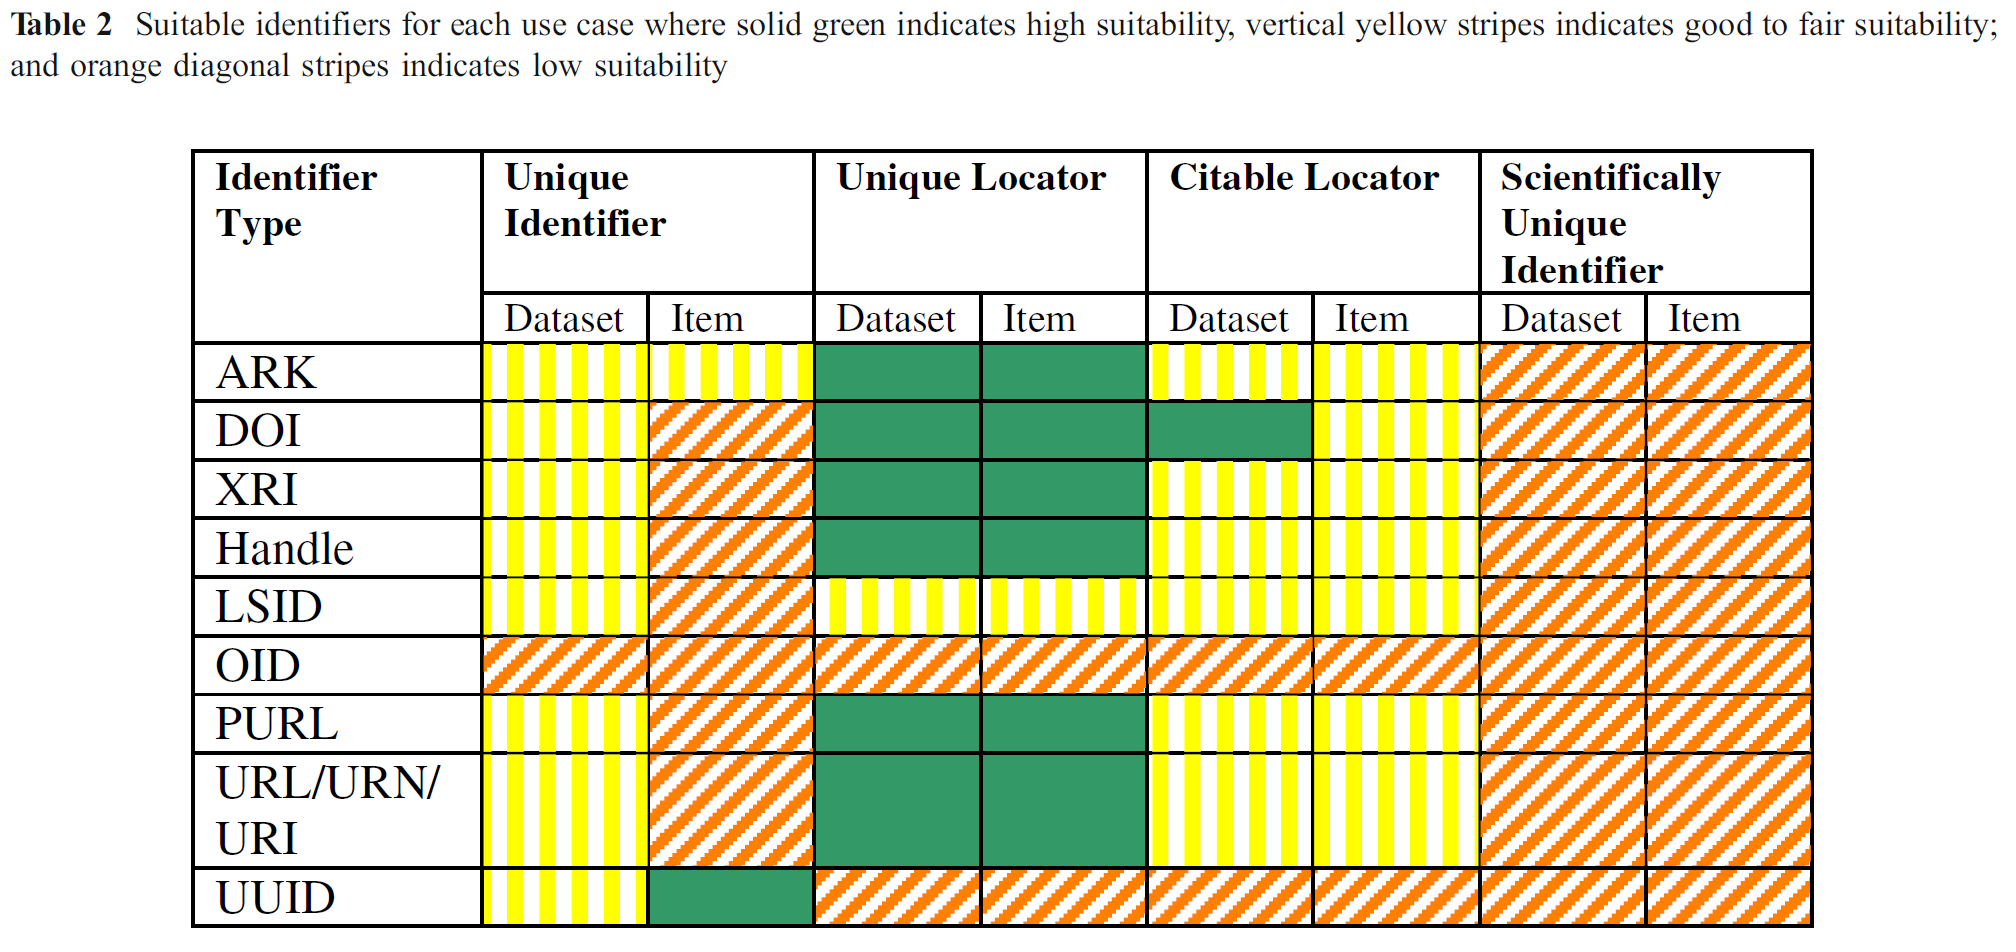
\includegraphics[scale=0.30]{figures/DigitalIdentifierTable.png}
	\caption[Table of predominant identifiers used in science.]{Table of predominant identifiers used in science.  From Duerr, et al. \cite{Duerr2011}}
	\label{table:Duerr}
\end{figure}
The DOI network provides a robust system to track documents, but when tracking data, it faces difficulty following the rate of change with more volatile data sets.
Under current definitions, distribution organizations assign different DOIs to separate editions of a document.
Documents often do not need new identifiers since they change very rarely as a result of the publication process.
Data set production and distribution cycles move more quickly and react more sensitively to small content changes, including when data collection continues on after initial publication.
Data set behavior becomes entirely too slow as data providers begin allowing users to dynamically generate data products from existing data according to their needs \cite{Barkstrom2003a}.
Some agencies have begun assigning versioned DOIs, but this has not become common practice.
Other groups do not assign a new DOI, but reference the latest release of the document or object \cite{Ands2017}.

As digital methods have evolved, so have digital libraries.
The documents that digital libraries store are no longer constrained by physical organization \cite{Barkstrom_digitallibrary}.
A book can physically be randomly stored for efficient retrieval, but the digital copy may reside in multiple locations depending on dynamic filters or search queries.
The Mellon Fedora Project developed a standardized edition control structure to unify disparate digital library stores \cite{Payette2002}.
The regularizing edition tracking methods significantly improved the response time and relevancy of the library services.

\subsection{Software Versioning}

Software versions form the most visible displays of versioning often experienced by researchers.
Version managers provide tools to archive and restore code through the development lifecycle.
The Revision Control System (RCS), developed in originally in 1985, documents one of the earliest uses of the dot-decimal identifier \cite{tichy1985rcs}.
This identifier uses a sequence of whole numbers concatenated by decimals.
The system possessed many features of modern SVMs such as branches, a separate copy of the code for developing changes safely, which were identified by extending the dot-decimal identifier as seen in Figure \ref{RCSTree}.
\begin{figure}
	\centering
	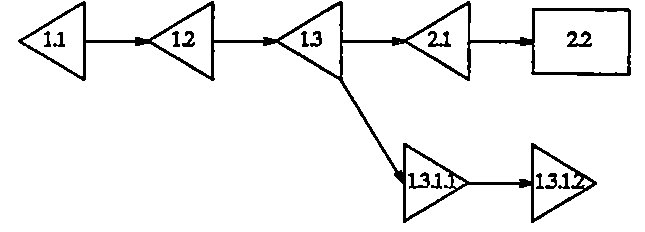
\includegraphics[scale=0.75]{figures/RCSCommitTree.png}
	\caption[Commit history of an object in RCS with changes in the main line stored as back deltas and side branches stored as forward deltas.]{Commit history of an object in RCS with changes in the main line stored as back deltas and side branches stored as forward deltas.  Figure 5 in \cite{tichy1985rcs}}
	\label{RCSTree}
\end{figure}
Not long after, the Concurrent Versions System (CVS) gained popularity with methods allowing multiple users to concurrently develop code to a central repository \cite{cederqvist2002version}.
The most popular modern SVM is GIT which also allows concurrent development but enables distributed repositories \cite{Chacon:2009:PG:1618548}.
Each developer contributing to a project is considered by the system to possess the master copy of that project.
The users collaborate by requesting and pulling other developer's master copies into their project.
In previous SVMs, only the differences between software files were stored, but GIT stores the entirety of each file version.
Figure \ref{GITFile} demonstrates an example of how GIT employs storage space for multiple versions \cite{Chacon:2009:PG:1618548}.
\begin{figure}
	\centering
	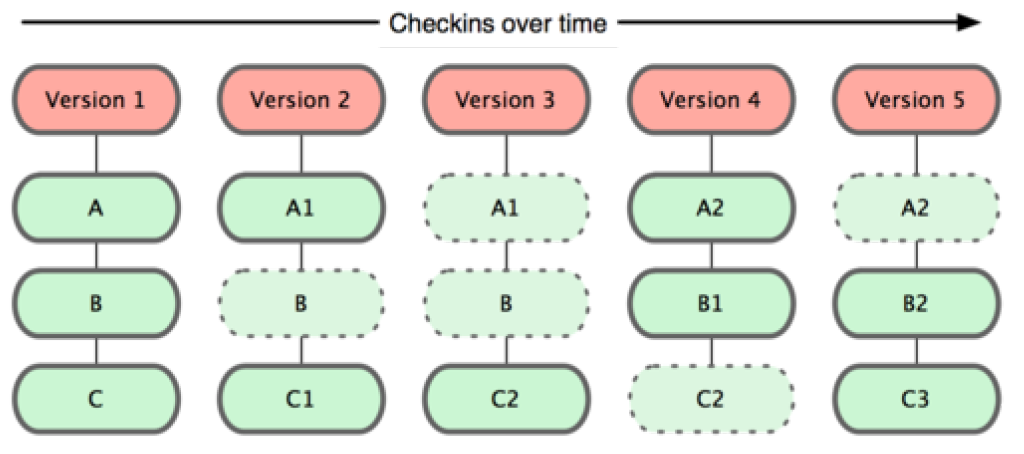
\includegraphics[scale=0.50]{figures/GITFiles.png}
	\caption[GIT stores changes in the repository as snapshots of individual files.]{GIT stores changes in the repository as snapshots of individual files. Figure 1.5 from \cite{Chacon:2009:PG:1618548}}
	\label{GITFile}
\end{figure}
Only a pointer is stored in subsequent versions for unchanged files, saving space.
Fischer, et al., demonstrate the importance of software version systems by integrating the manager with a bug tracking system to indicate the bugs a version release addresses \cite{Fischer2003}.

\subsection{Database Versioning}

The need for dta versioning methods grew alongside the growing popularity and power of relational databases.
Klahold, et al., introduced using abstract versioning environments in 1986 to separate the temporal features and organize the data into related groupings \cite{Klahold:1986:GMV:645913.671314}.
Research in the versioning area focused primarily on the database schema.
The results were temporal databases where schemas included time and dated transactions modifying the schema \cite{roddick1996model}.
Temporal databases allowed old queries to be executed on updated schemas, improving the reproducibility of results.
Capturing periodic snapshots or copies becomes unfeasible with increasingly large centralized database systems.
Data collection continues to migrate towards massive data warehouses which store and serve a wide variety of data \cite{Vassiliadis1999}.
Proell and Rauber have investigated tracking data queries instead of the database as a more scalable solution to reproduce data \cite{proellBigData}.
The queries can then be used as publication citations to provide scalable, reproducible references to older data \cite{Proell2013} \cite{DBLP:conf/data/2013}.

\subsection{Grid Versioning}

The grid provides a sensitive environment for versioning where there are many users and data movement across the grid should be avoided.
The CERN grid for the Compact Muon Solenoid experiment carefully developed processes which allow references by multiple users to the same file without copying that file across the grid \cite{Holtman:687353}.
Versions lock and release to permit parallel processing while still archiving additions and modifications to the data.
Grid versioning applications also begins to highlight the difference in versioning usage patterns between users and producers \cite{Branco2008}.
Deeper exploration into the ATLAS system documentation did not reveal specific use cases explaining the differences.
The grid also provides users with the ability to begin dynamically defining data sets to their needs by aggregating results from across the network \cite{Barkstrom2003a}.
The process would create new data sets without prior existing change documentation and fueled a demand for responsive frameworks which could track the discordant data collection conditions assimilated by the system \cite{Kovse2003VGridAVS}.

\subsection{Ontology Versioning}

Ontologies play a major role in defining domains, especially in the biological and medical fields where terms and definitions can change rapidly across highly variable organisms \cite{Ochs:2015:SVS:2826733.2826866}.
As a result, the ontologies require consistent methods to capture and model changes to evolving terms.
Tools aid in the process by detecting differences between ontologies \cite{Hartung201315}.
Klein and Fensel have found that when the changes are discovered, both forward and backward compatibility must be established for clear ontology versioning \cite{Klein01ontologyversioning}.
Not only must the path from an old term to a new one be clear, but a method for new terms to interact with old data must also exist.
They additionally identified three levels at which ontologies can differ: the domain, the conceptualization, and the specification.
Hauptmann et al., define a method to version ontologies natively within a triple store using linked data \cite{HauptmannEtAl:LDQ2015} \cite{LDQ2015}.
The method heavily relies on the context of stored data.


\section{Version Models} \label{sec:models}

Version models provide a visual a theoretical aid in understanding where a data object lies in relation to the rest of a work.
The Atmospheric Radiation Measurements (ARM) group used a model dividing the data into mathematical sets which versioning operations acted upon\cite{6906868}.
Adding files already in the set created a new set which inherited all non-intersecting files and included all the new ones.
The model provided a means to organize and automate the versioning of ARM's daily expanding data sets.

The Health Care and Life Sciences (HCLS) Interest Group of the World Wide Web Consortium (W3C) recently released a model which may provide a solution when used in conjunction with other identifiers \cite{Dummontier2016}.
Their model, shown in Figure \ref{HCLSModel}, separates the concept of a data set into three groupings.
\begin{figure}%[b]
	\centering
	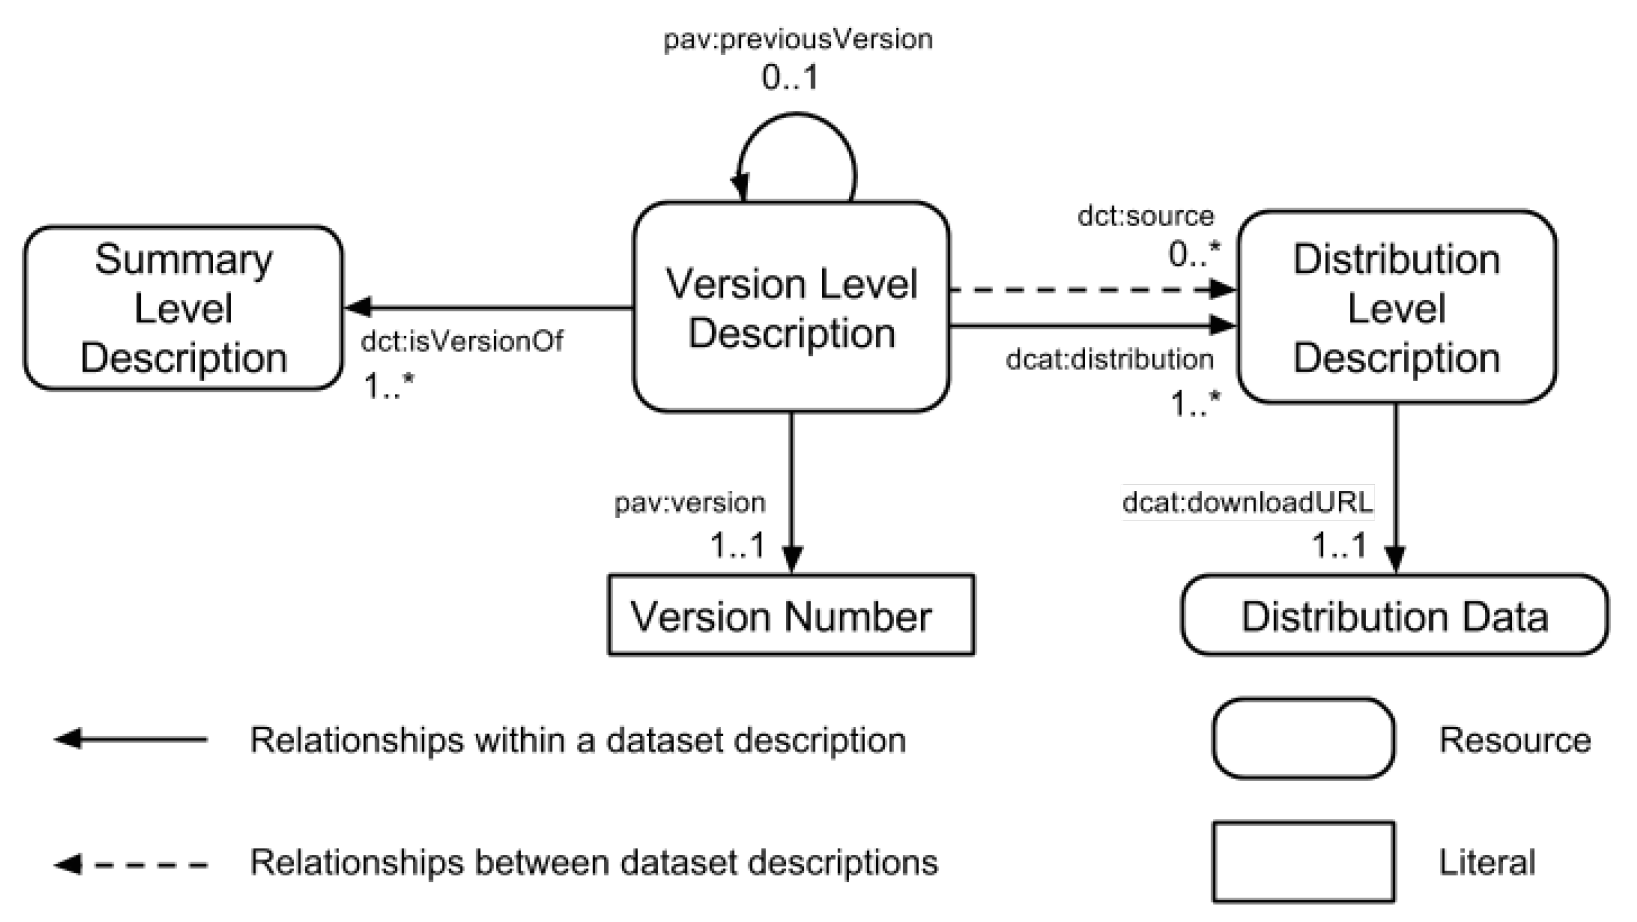
\includegraphics[scale=0.35]{figures/HCLSModel.png}
	\caption[Data model from the Health Care and Life Sciences Interest Group separating data into three levels: works, versions, and instances.]{Data model from the Health Care and Life Sciences Interest Group separating data into three levels: works, versions, and instances.  From Dummontier, et al. \cite{Dummontier2016}}
	\label{HCLSModel}
\end{figure}
The highest level summarizes the data as an abstract work, perhaps better described as a topic or title.
The data topic can have multiple versions over time.
The version can then be instantiated into various distributions with different physical formats.
The model---relating summary, version, and distribution---also strongly resembles the formation of FRBR's work, expression, and manifestation model.

\begin{figure}
	\centering
	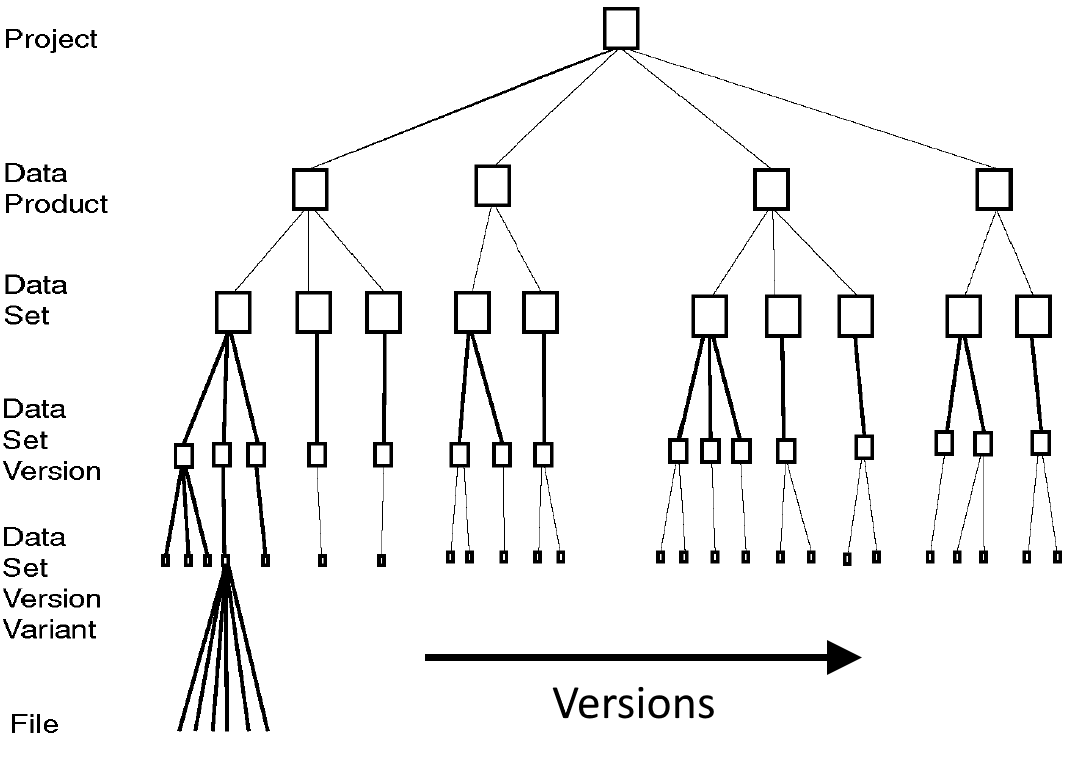
\includegraphics[scale=0.50]{figures/hierarchy.png}
	\caption[Visual representation of grouping hierarchy.]{Visual representation of grouping hierarchy.  From \cite{Barkstrom2003}}
	\label{hierarchy}
\end{figure}

From his definition of versions, Barkstrom also outlines an hierarchical version model as seen in Figure \ref{hierarchy}.
The model features additional intermediary levels than the HCLS's model, following NASA's data curation practices \cite{barkstrom2014earth}.
Each edge in the tree signifies a difference with other objects at the same depth, but the model does not provide a mechanism to explain the difference.

\section{Provenance Ontologies}

Provenance ontologies form a major section of linked data approaches to data versioning.
The coverage stems from the close relation between provenance and differentiating versions.
The Proof Markup Language, one of the first semantic models to capture provenance information, expressed lineage relationships using inference reasoning through traceable graphs \cite{daSilva2006381}.
The technique provides a powerful way to express and imply sequences of relationships between different versions and characterize the manner of their relation.

\subsection{Open Provenance Model}

A number of linked data models include versioning concepts such as the Open Provenance Model (OPM) \cite{moreau2008open}.
Driven by the uncertain needs and sometimes conflicting conventions of different scientific domains, the model sought to find a method to standardize the way in which provenance data is captured while also keeping the specification open to accommodate current data sets through the change.
In an experimental case, the model has been applied to sensor networks, automating and unifying their provenance capture even as they grow \cite{5478496}.
To aid OPM's adoption, the framework Karma2 integrates provenance capture into scientific workflows and provides a more abstract view of their data collection activities \cite{simmhan2010karma2}.
The property \textit{opm:WasDerivedFrom} constitutes a core concept in the model and marks the reliance of one object's existence on another object.
For a large part, this encompasses the engagement which provenance models view versions, without further need to explore the derivation's content.

\subsection{PROV-O}\label{sec:prov}

PROV, a World Wide Web Consortium (W3C) Recommendation, delineates a method to express data provenance in a more compact form as seen in Figure \ref{PROVO} \cite{Gil2013a} \cite{Groth2013}.
\begin{figure}
	\centering
	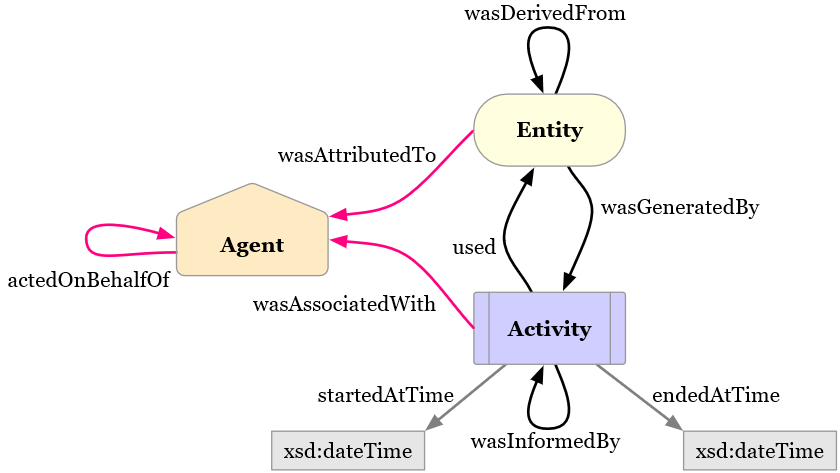
\includegraphics[scale=0.5]{figures/ProvO.png}
	\caption[Diagram of the PROV Ontology.]{Diagram of the PROV Ontology.  Figure 1 from \cite{Lebo2013}}
	\label{PROVO}
\end{figure}
The recommendation uses a conceptual model relating activities, agents, and entities to describe data production lineage \cite{Moreau2013c} \cite{Nies2013} \cite{Nies2013a}.
Intended as a high level abstraction, it takes an activity-oriented approach to provenance modeling.
Every data entity results from the actions of some activity \cite{Gil2013}.
The conceptual model's expression occurs through the PROV Ontology (PROV-O), which can be conveyed through various resource description languages \cite{Hua2013} \cite{Klyne2013}.
The ontology is further formalized into a functional notation for easier human consumption \cite{Moreau2013b} \cite{Cheney2013a}.
One particular strength that has contributed to the adoption of PROV is its ability to link into other ontologies, making it easier for existing semantically enriched data sets to adopt PROV \cite{Miles2013} \cite{Moreau2013}.

PROV has provided a major contribution in maintaining the quality and reproducibility of data sets and reporting in the National Climate Assessment (NCA) \cite{Ma2014191}.
The contribution signifies that there is an increased likelihood of adoption through other scientific fields as a result of this reporting.
The Global Change Information System, which houses the data used to generate the NCA, uses PROV to meticulously track the generation of its artifacts and results as they are used in assessment report \cite{Tilmes2012}.
The usage means that not only does the data have a traceable lineage to verify quality, but the content of documents can have the same verifiability \cite{Ma2014}.
Komadu, a framework developed to alleviate workflow integration, utilizes PROV to improve upon its predecessor, Karma, by no longer utilizing global context identifiers that were not necessarily shared throughout the workflow. \cite{Suriarachchi_2015}.

The PROV Ontology provides three different concepts that begin to encapsulate the provenance relationship between data versions.
It defines a \textit{prov:Generation} as "the completion of production of a new entity by an activity," \cite{Lebo2013}.
This means that the generation, which corresponds adding an object to a version, must result from a \textit{prov:Activity}.
\textit{Prov:Invalidation}, defined as the, ``start of the destruction, cessation, or expiry of an existing entity by an activity," makes a similar connection between activities and entities \cite{Lebo2013}.
A third concept, \textit{prov:Derivation}, relates two entities, and the ontology defines it as, "a transformation of an entity into another, an update of an entity resulting in a new one, or the construction of a new entity based on a preexisting entity. " \cite{Lebo2013}.
PROV also has a property called \textit{prov:isDerivedFrom} which conveys the same definition as a \textit{prov:Derivation}.
Using the property and concept together forms a qualified property which can be instantiated and further annotated.

\subsection{Provenance, Authorship, and Versioning Ontology}

The Provenance, Authorship, and Versioning (PAV) Ontology is, ``a lightweight vocabulary, for capturing ``just enough" descriptions essential for web resources representing digitized knowledge" \cite{Ciccarese2013}.
It provides a means to track versioning information through linked data by introducing \textit{pav:version} to cite versions and \textit{pav:previousVersion} to link them together in order \cite{Ciccarese2013}.
It does so in comparison to the Dublin Core concept \textit{dc:isVersionOf} which records, "Changes in version imply substantive changes in content rather than differences in format" \cite{DCMI2012}.
PAV supports the idea that a new concept becomes necessary to cover cases where new versions do not have to be substantive but can still be alternate editions of the original object.
While it documents related versions well, PAV does not dive deeper in explaining the circumstances behind version differences.

\subsection{Schema.org}

The Schema.org ontology is not a provenance ontology but provides a means to supply searchable web pages with standardized micro-data.
The ontology has a collection of concepts which could be applied to versioning.
The \textit{schema:UpdateAction} is defined as, ``the act of managing by changing/editing the state of the object," which encompasses the same responsibilities expected of versioning systems \cite{Schema}.
The terms \textit{schema:AddAction}, \textit{schema:DeleteAction}, and \textit{schema:ReplaceAction} subclass the \textit{shcema:UpdateAction}.
These classes model actions which further cement parallels between versioning and \textit{schema:UpdateAction}.

Schema.org defines a \textit{schema:ReplaceAction} as, ``the act of editing a recipient by replacing an old object with a new object" \cite{SchemaRep}.
The concept has two properties, \textit{schema:replacee} and \textit{schema:replacer} which indicates that a new object replaces an old one.
Schema.org models the interaction by placing the replacement action at the relation's center.
In comparison, the \textit{schema:AddAction} is defined as, ``the act of editing by adding an object to a collection" \cite{SchemaAdd}.
The action only involves the object and the new state of the collection, not involving any of the collection's prior lineage.
Schema.org defines the \textit{schema:DeleteAction} as, "the act of editing a recipient by removing one of its objects," \cite{SchemaRem}.
The concept aligns well with other versioning systems, although deletion may be a strong assertion.

\section{Change Logs} \label{sec:changelog}

Change logs, artifacts resulting from the versioning process, play a major role filling in gaps between versions.
The logs document changes and explain, in human language, motivations behind the modifications \cite{uel1037}.
Since identifiers denote that a change has occurred, the logs provide details on how the changes modify an object's attributes.
They demonstrate a need and utility in understanding the deeper content of change beyond knowing that an object did transform.
While some data sets will provide a change log, software projects have normalized their use in version release documentation.
As a result, these projects provide a basis for understanding the value these logs can supply data sets with multiple versions.
The change log's common drawback is the limitation to only human readable text.
Wider adoption among data sets may be possible by making these texts machine computable.

Open source projects use change logs more consistently than data projects, which usually sport only use documentation.
Logs play an important communication role in these projects since developers can contribute without having been part of the original development team.
The change logs allow developers to link bugs and errors with their corrections in new versions of the code \cite{Chen:2004:OCL:990374.990391}.
The links gives insight into motivations behind particular design decisions.
Logs linked with version releases also provide feedback to the user community that corrections have been addressed, in addition to ensuring that improvements drive modifications to the code base.
An identifier cannot communicate these qualities while remaining succinct.
Some research has been done to determine the health of a development project based on the number and length of change logs released over time \cite{German03automatingthe}.
Little work has been done to make change logs machine-computable, as many of these documents remain in human-readable text only.
Research done involving change log content must manually link entries with computable meta-data such as the introduction of new features with the emergence of new bugs \cite{6132954}.
While machines may still be significantly removed from the ability to comprehend the impact of changes made to a data set or software code, they are currently opaquely blocked from consuming any of the content within logs more than understanding they contain text.
The transition between different versions of large data sets is then left largely up to the human user's ability to understand and process the modifications mentioned within the change log.

\section{Introduction of Use Cases}

\subsection{Use Case 1: Linked Data Change Log}
Needed a project with at least two versions, and the objects had to have content differences.
The single project constraint makes sure they're from the same work.
Excel spreadsheets allow simultaneous instances of each version and well supported tools for access.

\subsection{Use Case 2: Multi-version Change Distance}

\section{Hypothesis Statement}

Large data collection endeavors necessitate the development and deployment of versioning systems to manage change propagating through their data.
Advancing beyond identifier comparisons and delving into capturing substantive change can significantly improve the ability to standardize version communications and transition.
The work in the following chapters will contribute to expanding change capture by defining a more expressive linked data versioning model.
The model will allow current versioning documentation to become machine-consumable.
A better method will be developed to provide a quantitative basis for the assignment of version identifiers.

\section{Contributions}


%%% Local Variables:
%%% mode: latex
%%% TeX-master: t
%%% End:
 % Introduction
%%%%%%%%%%%%%%%%%%%%%%%%%%%%%%%%%%%%%%%%%%%%%%%%%%%%%%%%%%%%%%%%%%%
%                                                                 %
%                            CHAPTER TWO                          %
%                                                                 %
%%%%%%%%%%%%%%%%%%%%%%%%%%%%%%%%%%%%%%%%%%%%%%%%%%%%%%%%%%%%%%%%%%%

\chapter{PREVIOUS WORK}\label{ch:prevwork}
%\resetfootnote %this command starts footnote numbering with 1 again.

The data versioning landscape produces a variety of different approaches and standards towards change capture.
However, massive centralized data stores have become more prevalent as data distribution methods advance  \cite{Vassiliadis1999}.
Collection into larger unified repositories will likely require a multi-tiered approach to synchronize the varied practices  \cite{Baker2009}.
Baker notes that differences depend on the sociotechnical distance of a repository from the data's origin \cite{Baker2009}.
Local stores closer to the collection site better understand data capture conditions, but must also adapt to changing environments.
Science agencies and organizations are only beginning to formally codify and standardize methods to capture and publish lineage information \cite{MatthewS.Mayernik201312-039}.
This seems to be a recurring cycle of attention with rapidly developing technologies such as the grid or parallel computing \cite{Kovse2003VGridAVS}.
The CERN grid for the Compact Muon Solenoid experiment carefully developed necessary processes which allow references by multiple users to the same file without copying that file across the grid \cite{Holtman:687353}.

The model defined in Chapter \ref{ch:model} provides a basis for understanding the formal underlying properties which will allow consistent versioning practices.
Previous work in provenance, provenance distance, and mapping provide inspiration for the model's form.
A majority of the linked data approaches to version capture can be found in provenance models.
Additionally, researchers have attempted to address the amount of change between version identifiers using a measure called provenance distance.
This distance measure lacks sufficient resolution to provide detailed quantities to answer many versioning questions.
The model also draws inspiration from existing change mapping methods found in version control managers to reduce space consumption when working with large data sets.
These mapping methods provide a familiar and regularized basis to both compute and present changes.

\section{Provenance}

A number of linked data models include versioning concepts such as the Open Provenance Model (OPM) \cite{moreau2008open}.
Driven by the uncertain needs and sometimes conflicting conventions of different scientific domains, the model sought to find a method to standardize the way in which provenance data is captured while also keeping the specification open to accommodate current data sets through the change.
In an experimental case, the model has been applied to sensor networks, automating and unifying their provenance capture even as they grow \cite{5478496}.
To aid OPM's adoption, the framework Karma2 integrates provenance capture into scientific workflows and provides a more abstract view of their data collection activities \cite{simmhan2010karma2}.
The property WasDerivedFrom constitutes a core concept in the model and marks the reliance of one object's existence on another object.
For a large part, this encompasses the engagement which provenance models view versions, without further need to explore the derivation's content.

PROV, a World Wide Web Consortium (W3C) Recommendation, delineates a method to express data provenance in a more compact form as seen in Figure \ref{PROVO} \cite{Gil2013a} \cite{Groth2013}.
The recommendation uses a conceptual model relating activities, agents, and entities to describe data production lineage \cite{Moreau2013c} \cite{Nies2013} \cite{Nies2013a}.
Intended as a high level abstraction, it takes an activity-oriented approach to provenance modeling.
Every data entity results from the actions of some activity.
The conceptual model's expression occurs through the PROV Ontology (PROV-O), which can be conveyed through various resource description languages \cite{Hua2013} \cite{Klyne2013}.
The ontology is further formalized into a functional notation for easier human consumption \cite{Moreau2013b} \cite{Cheney2013a}.
One particular strength that has contributed to the adoption of PROV is its ability to link into other ontologies, making it easier for existing semantically enriched data sets to adopt PROV \cite{Miles2013} \cite{Moreau2013}.
\begin{figure}
	\centering
	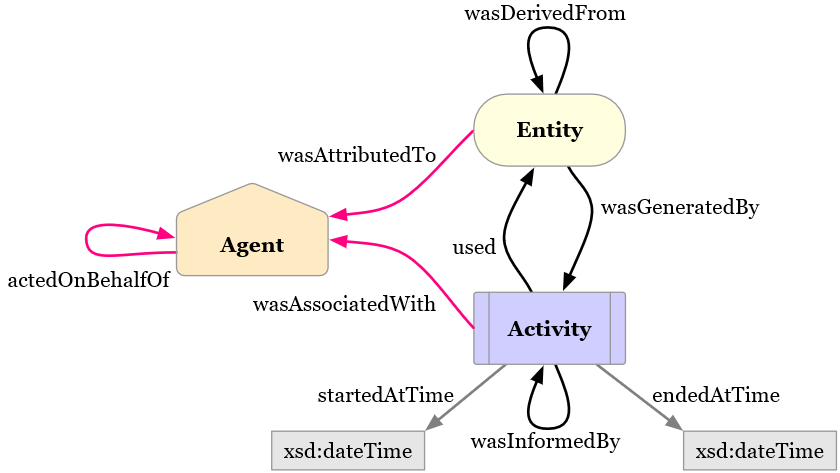
\includegraphics[scale=0.5]{figures/ProvO.png}
	\caption[Diagram of the PROV Ontology.]{Diagram of the PROV Ontology.  Figure 1 from \cite{Lebo2013}}
	\label{PROVO}
\end{figure}
Komadu, a framework developed to alleviate workflow integration, improves upon its predecessor, Karma, by no longer utilizing global context identifiers that were not necessarily shared throughout the workflow. \cite{Suriarachchi_2015}.


The PROV Ontology provides three different concepts that begin to encapsulate the provenance relationship between data versions.
It defines a \textit{prov:Generation} as "the completion of production of a new entity by an activity," \cite{Lebo2013}.
This means that the generation, which corresponds to the version addition operation, must result from a \textit{prov:Activity}.
However, activities play a much less active role in versioning since object comparisons instead expose changes.
The property creates a relationship between entities and activities, but such a connection may imply that perturbations in the activity resulted in changing the version.
Changes could also result from modifications in the input data, leading to an entirely new generating activity rather than a modified one.
\textit{Prov:Invalidation} likewise makes a similar connection between activities and entities.
This means that PROV-O does not have the direct means to communicate the addition and invalidation relationships which exist in our versioning context.
Since we previously establish a state-based view between versions, a more contextually appropriate property should connect two objects together.
Continuing, \textit{prov:Derivation} does relate two entities and the ontology defines it as, "a transformation of an entity into another, an update of an entity resulting in a new one, or the construction of a new entity based on a preexisting entity. " \cite{Lebo2013}.
In the Marine Biodiversity Virtual Laboratory (MBVL) data set's case described in Section \ref{sec:MBVL}, none of these three assertions hold true. 
The process simultaneously considers all four versions so one is not transformed into another as would a sequential set of versions.
Additionally, since we do not know which version is the best, we cannot consider any data set as an update of the others.
Finally, no entity preexisted as the data sets resulted from an ongoing analysis and further steps have not been developed.

The Provenance, Authorship, and Versioning (PAV) Ontology is, "a lightweight vocabulary, for capturing ``just enough” descriptions essential for web resources representing digitized knowledge" \cite{Ciccarese2013}.
It provides a means to track versioning information through linked data by introducing \textit{pav:version} to cite versions and \textit{pav:previousVersion} to link them together in order \cite{Ciccarese2013}.
It does so in comparison to the Dublin Core concept \textit{dc:isVersionOf} which records, "Changes in version imply substantive changes in content rather than differences in format" \cite{DCMI2012}.
PAV supports the idea that a new concept becomes necessary to cover cases where new versions do not have to be substantive but can still be alternate editions of the original object.
While it documents related versions well, PAV does not dive deeper in explaining the circumstances behind version differences.

The Schema.org \textit{schema:UpdateAction} largely reflect the relationships adopted by this work, and are defined as "the act of managing by changing/editing the state of the object" \cite{Schema}.
The remaining subclasses include the \textit{schema:AddAction}, \textit{schema:DeleteAction}, and \textit{schema:UpdateAction}.
The function of these terms is to provide a means to supply searchable web pages with standardized micro-data.
As a result, they orient their properties towards definitions and characterization but do not provide the right structure for a standardized change capture model.

\section{Provenance Distance}

With increasing complexity, data workflows have developed in such a way that even subtle changes have serious implications for other parts of the workflow \cite{TILMES2011548}.
This observation makes change impact difficult to measure, but one insight begins with provenance's role in workflows.
Provenance can give great insight into a data object's future performance such as the  ability to predict disk usage based on the lineage of a data object \cite{dai2014provenance}.
Efforts have also been made to summarize provenance representations to improve consumption \cite{Ainy:2015:ASD:2806416.2806429}.
Changes to the process creating an object signals the development of a new version.
Therefore, studying the magnitude of this deviation should give some idea into the resulting object's impact.
This idea, known as provenance distance, seeks to determine the impact of changes in provenance on new data versions through measuring graph edit distances.

\begin{figure}
	\centering
	\begin{adjustbox}{addcode={\begin{minipage}{\width}}{
					\caption[Provenance graph of a Level 3 data product, showing the inter-relations between different data products in generating the final product.]{Provenance graph of a Level 3 data product, showing the inter-relations between different data products in generating the final product.  Figure 2 from \cite{TILMES2011548}}\end{minipage}},rotate=90,center}
		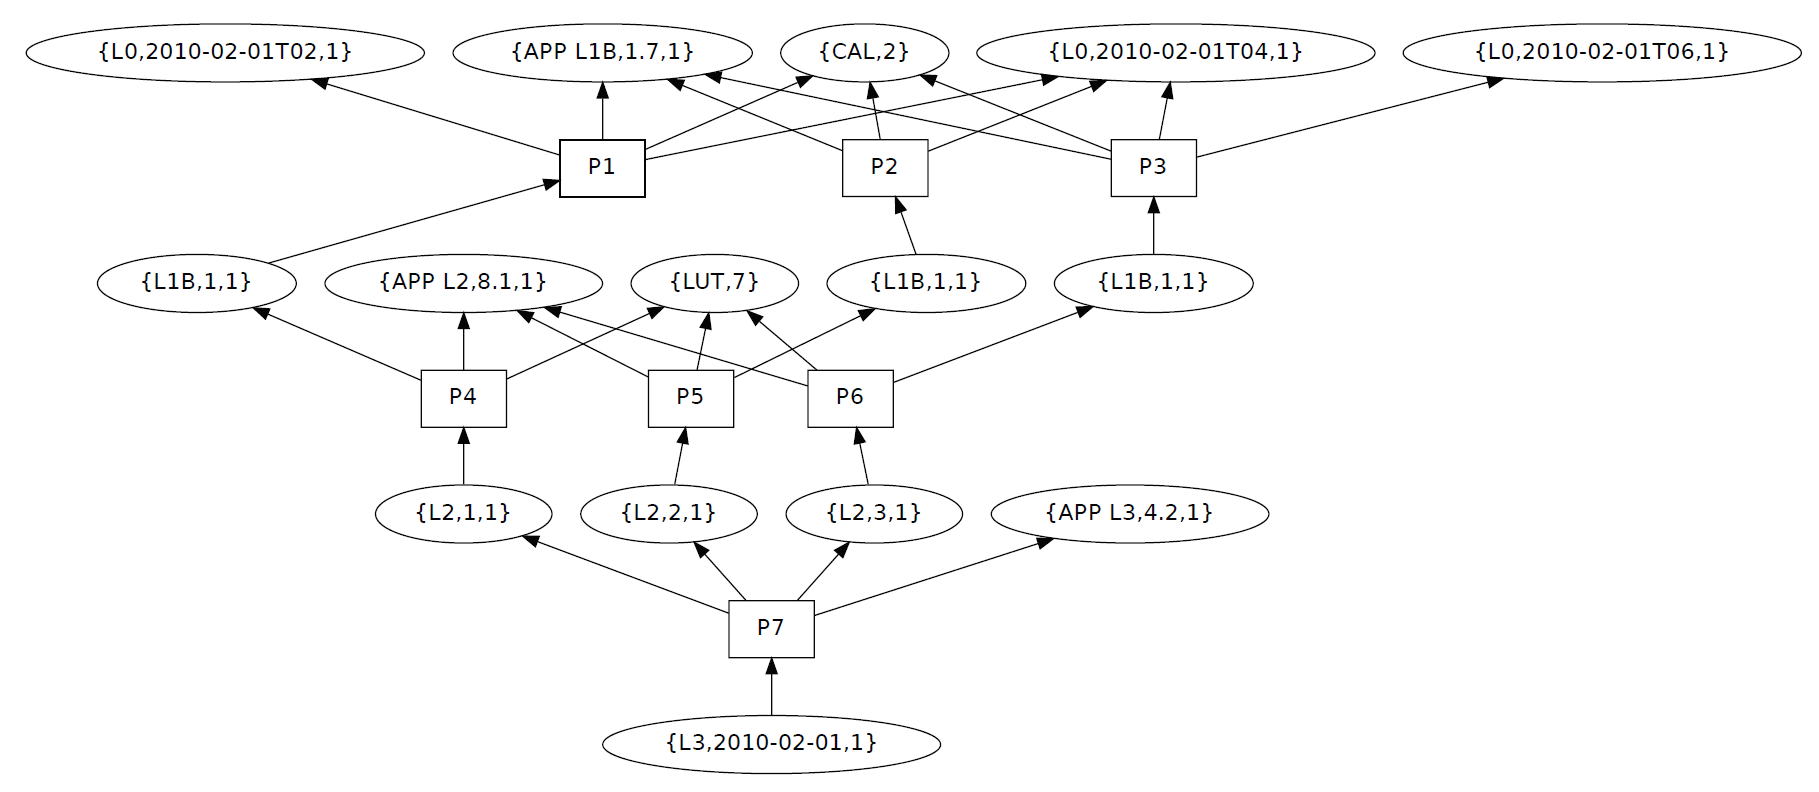
\includegraphics[scale=0.5]{figures/OzoneProvGraph.png}
	\end{adjustbox}
	\label{ProvGraph}
\end{figure}

The first ingredient necessary to calculate provenance distance is a linked data graph capturing the sequence of events leading to the old and new objects' creation, like the one shown in Figure \ref{ProvGraph}.
It shows the multiple lower level products involved in creating a Level 3 ozone indicator.
This can be accomplished through the use of previously mentioned provenance models, but these graphs are not widely available.
Using PROV to represent provenance data in a semantic model produces an acyclic directed graph with labeled nodes.
As a result, the provenance distance problem reduces to similarity measurement.
When calculating this measure, algorithms determine how far two graphs are from being isomorphic \cite{Cao2013}.
Node labeling simplifies this process by providing nodes which must match together, and greatly reduces the complexity from computing generalized graphs.
Graph Edit Distance, counting the edits necessary to transform one graph into another, provides a quantitative measure to associate with this process  \cite{Gao2010}.
Some variations count edge changes \cite{Goddard:1996:DGU:246962.246972}.

In Figure \ref{GraphEdit}, the left graph transforms through a move of edge 1 and a rotation of edge 4, resulting in an edit distance of two.
Such changes in a provenance graph would demonstrate an alteration in dependencies between objects used to generate a final notable product.
This kind of analysis resembles comparison measures employed in determining semantic similarity \cite{Hliaoutakis06informationretrieval}.
However, isolating changes responsible for differences in provenance can become difficult in complex environments as Tilmes observes in 2011, 
\begin{quotation}
	Consider the relatively common case of the calibration table, which is an input to the L1B process, changing. Even though the version of the L2 or L3 software hasn't changed, the data files in the whole process have been affected by the change in the calibration.
\end{quotation} \cite{TILMES2011548}.
L-number is shorthand for the level system featured in Figure \ref{NASALevels}.
While provenance distance may be straight-forward to calculate, the indicator hides many insights into an object's behavior.

\begin{figure}
	\centering
	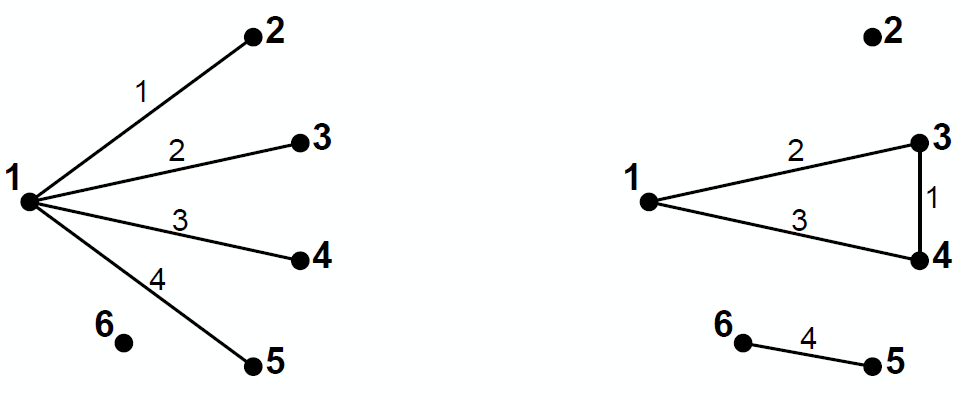
\includegraphics[scale=0.40]{figures/GraphEdit.png}
	\caption[The labeled graph on the left transforms into the right graph under two edge edits.]{The labeled graph on the left transforms into the right graph under two edge edits. Figure 2 from \cite{Goddard:1996:DGU:246962.246972}}
	\label{GraphEdit}
\end{figure}

Methods to provide quality of service boundaries leveraging provenance already exist which compare workflows based on performance criteria \cite{2015:CAA:2778374.2778504}.
However, these procedures focus primarily on quick retrieval and efficient storage instead of capitalizing on the latent information accessed by reasoning across data set versions \cite{tan2004research}.
The distance measures previously mentioned rely solely on provenance graphs to compute results, but this is obviously insufficient.
When considering the provenance of a data object, methods only consider the activities and entities that took an active role in the production of it.
A new version of an object has a familial relationship with its previous versions, but in most cases, they do not take an active role in its generation.
Without detailed change information, determining the difference between two data objects in a metric beyond broad strokes becomes difficult, if not impossible.

As per our definition of `version', objects must have common provenance, and the more similar they are, the more meaningful the results from versioning methods.
Provenance distance provides a means of determining how reliable versioning results are given a greater adoption of provenance graphs.
Measuring a change's impact with accuracy comparable to a change log requires a more detailed understanding and description than provenance can provide  \cite{Bose:2005:LRS:1057977.1057978}.
Sufficiently precise versioning measurements cannot be provided by provenance distance, but it could indicate the confidence of versioning results, which is out of scope for this project.

\section{Mapping}

Data managers primarily use one of two methods to store data versions: snapshots and deltas.
The snapshot method makes periodic copies of the data's state at a point in time.
While storing and retrieving these snapshots can be very quick, they require significant amounts of space to maintain.
The software manager GIT employs this method and Figure \ref{GITFile} demonstrates an example storage space for multiple versions \cite{Chacon:2009:PG:1618548}.
The squares with dotted outlines indicate unmodified files, which the system stores as pointers instead of full objects.
In addition, GIT compresses and separately stores very old versions which are unlikely to be accessed.
This versioning style may not be ideal for larger or often modified data sets as the size requirements will quickly grow unmanageable.
However, for many library or catalog environments, they cannot predict the target volume a user desires and must prioritize availability \cite{Payette2002} \cite{Barkstrom_digitallibrary}.
Some methods like the inverted file index have been developed to balance space and retrieval performance on web documents, especially since wikis and news feeds have grown in deployment \cite{Berberich:2007:TMT:1277741.1277831}.
Searches over these text media may require execution on older archived web pages.

\begin{figure}
	\centering
	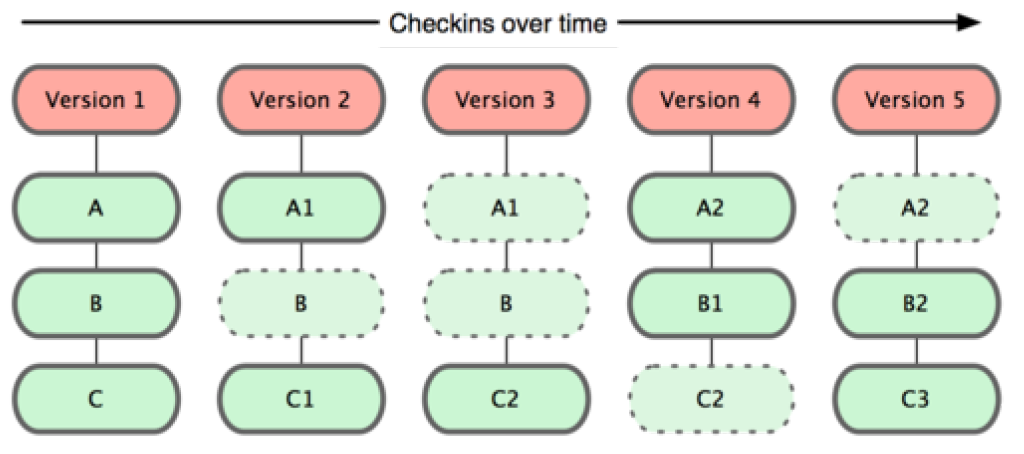
\includegraphics[scale=0.50]{figures/GITFiles.png}
	\caption[GIT stores changes in the repository as snapshots of individual files.]{GIT stores changes in the repository as snapshots of individual files. Figure 1.5 from \cite{Chacon:2009:PG:1618548}}
	\label{GITFile}
\end{figure}

The delta method entails calculating and storing only the differences between one version and the next.
Back delta variations store a snapshot of the most recent version and compute deltas towards older releases.
The forward delta variation stores the oldest data's snapshot and has deltas going forwards.
This method uses the minimum amount of space but trades it in for computation time to recreate any given version.
Particularly long running versioning systems occasionally save an intermittent snapshot to cut down on this processing time.
The setup proves ideal for data sets which prioritize service to their most recent versions \cite{Stuckenholz:2005:CEV:1039174.1039197}.
Because change documentation captures information between version objects, they most resemble differences calculated by the delta method.

Properly detecting changes in a system's files allows file managers to correctly group them into versions as seen in research conducted by the Atmospheric Radiation Measurements (ARM) group \cite{6906868}.
Difference or diff applications must first properly map data between objects and align them for comparison.
Many text-based data sets rely on well-established algorithms to perform this alignment  \cite{Chien:2000:VMX:646544.696357} \cite{Hartung201315}.
Sequential scientific data largely avoids this problem since developers already know the files or objects they replaced.
However, users do not have this advantage and system managers are starting to recognize the difference in versioning usage patterns between users and producers \cite{Branco2008}.
Mayernik, et al., probably gives the best description saying, "Prospective records document a process that must be followed to generate a given class of products whereas retrospective records document a process that has already been executed" \cite{MatthewS.Mayernik201312-039}.
While producers take a retrospective approach to version usage, consumers of new versions must take a prospective view, adapting to new changes.
This indicates that the orientation of versioning information reflects the imagined customer of that data.


%%% Local Variables:
%%% mode: latex
%%% TeX-master: t
%%% End:
 % Literature Review
%%%%%%%%%%%%%%%%%%%%%%%%%%%%%%%%%%%%%%%%%%%%%%%%%%%%%%%%%%%%%%%%%%%
%                                                                 %
%                            CHAPTER THREE                        %
%                                                                 %
%%%%%%%%%%%%%%%%%%%%%%%%%%%%%%%%%%%%%%%%%%%%%%%%%%%%%%%%%%%%%%%%%%%

\chapter{CONCEPTUAL MODEL}\label{ch:model}

The conceptual model used within this thesis is built around the expression of three core versioning operations: addition, invalidation, and modification.  These three activities can be represented by interacting with three types of concepts: versions, attributes, and changes.  Versions represent the data entities being compared.  These could be two different editions of a book or versions of software.  It is important to understand that a version is an abstraction as it can be represented by multiple physical files.  In the sections that follow, operations will only consider the interaction between two versions and will be explained later in the chapter.  Versions then contain attributes representing a quantity being modified.  Specifically for tabular data, attributes would correspond to an identifier that refers to particular rows or columns within the data.  Attributes of the two versions are then connected by a change.  This link functions as a very general concept which can be subclassed into more informative types such as unit changes, improving the expressiveness of the model beyond PROV's revisionOf concept.

\section{ADDITION}

When a change adds a new attribute to a version, it only needs to refer to version two and its corresponding attribute.  The reasoning should be fairly obvious as the attribute never existed in version one, and therefore, there is nothing to refer to and no need to form a relationship between the change and version one.  However, by linking the addition change to version one, we address a difficulty with comparing provenance graphs.  When two data objects have identical structures, it is difficult to determine what time the objects were added to the dataset and which version they belong to.  As a result, determining the compatability of the two objects becomes difficult.  The change contributions to the dataset evolution appears naturally using this construction. The resulting model can be seen in Figure~\ref{AdditionFig}.  Some relationships are specifically left out, such as that between Change A and Version 2, to not confuse identification of other types of changes.  The relationship between Change A and Version 2 can still be implied from Attribute 2.

\begin{figure}[t]
	\centering
	\vspace{0.0in} % normally the command here would be \includegraphics
%	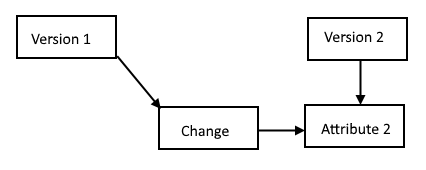
\includegraphics{figures/Addition.png}
	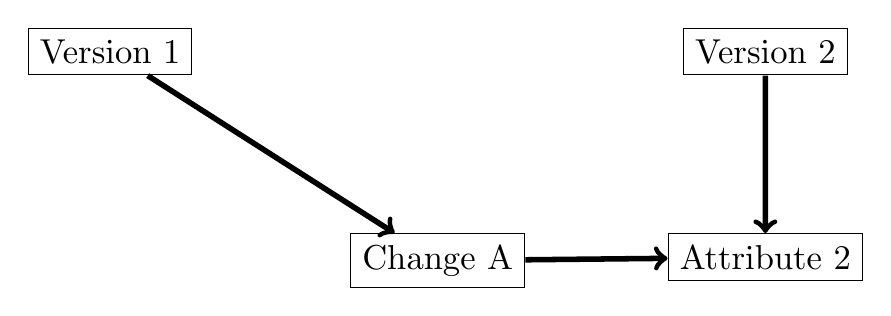
\begin{tikzpicture}[every node/.style={draw, rectangle}]
		\begin{scope}[node distance=20mm and 20mm]
			\node (c) [scale=1.25] at (1,0) {Change A};
			\node (1) [above left=of c, scale=1.25] {Version 1};
			\node (2) [above right=of c, scale=1.25] {Version 2};
			\node (a) [below =of 2, scale=1.25] {Attribute 2};
			
			\draw [line width=2pt,->] (1) -- (c);
			\draw [line width=2pt,->] (c) -- (a);
			\draw [line width=2pt, ->] (2) -- (a);
		\end{scope}
	\end{tikzpicture}
	\caption{Model of the relationships between Versions 1 and 2 when adding an Attribute 2 to Version 2 as a result of Change A}
	\label{AdditionFig}  % the \label command comes AFTER the caption
\end{figure}



\section{INVALIDATION}

The Invalidation operation corresponds to the delete concept found in other applications.  The choice of invalidation over delete results from the policy that, in versioning, data should never be deleted.  In practicality, this may not be particularly feasible due to space limitations and relative validity.  In either case, the change invalidates an attribute in version one, resulting in version two.  Unlike the Addition operation, Invalidation forms a clear relationship between both versions, which can be seen in Figure \ref{InvalidationFig}.  Notice again that since Attribute 1 no longer exists in Version 2, there is no corresponding Attribute 2 to refer to.

From Figure \ref{AdditionFig}, we can see the confusion that could result from requiring explicit relationships between versions and changes in both the Addition and Invalidation operations.  Linking Change A to Version 2 would create a duplicate connection and provides a mechanism to identify when items specifically enter or leave a version.

\begin{figure}[t]
	\centering
	\vspace{0.0in} % normally the command here would be \includegraphics
	%	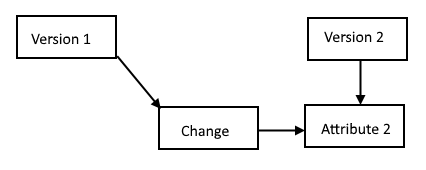
\includegraphics{figures/Addition.png}
	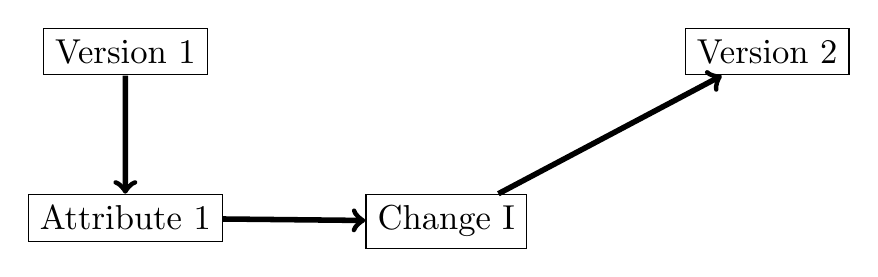
\begin{tikzpicture}[every node/.style={draw, rectangle}]
	\begin{scope}[node distance=15mm and 20mm]
	\node (c) [scale=1.25] at (1,0) {Change I};
	\node (1) [above left=of c, scale=1.25] {Version 1};
	\node (2) [above right=of c, scale=1.25] {Version 2};
	\node (a) [below =of 1, scale=1.25] {Attribute 1};
	
	\draw [line width=2pt,->] (a) -- (c);
	\draw [line width=2pt,->] (c) -- (2);
	\draw [line width=2pt, ->] (1) -- (a);
	\end{scope}
	\end{tikzpicture}
	\caption{Model of the relationships between Versions 1 and 2 when invalidating Attribute 1 from Version 1 as a result of Change I}
	\label{InvalidationFig}  % the \label command comes AFTER the caption
\end{figure}


\section{MODIFICATION}

The final operation is Modification, and it maps a change from one attribute from version one to its corresponding attribute in version two.  The particular type of change in this case is purposely left out in order to allow data producers to subclass and customize the resulting graph to properly reflect the versioning that they desire.

\begin{figure}[b]
	\centering
	\vspace{0.0in} % normally the command here would be \includegraphics
	%	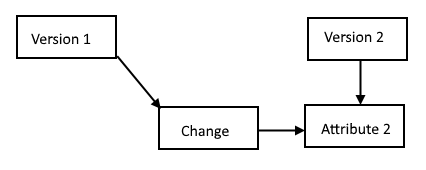
\includegraphics{figures/Addition.png}
	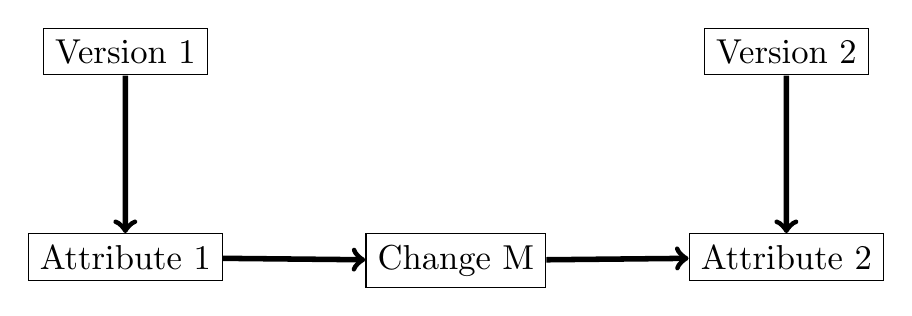
\begin{tikzpicture}[every node/.style={draw, rectangle}]
		\begin{scope}[node distance=20mm and 20mm]
			\node (c) [scale=1.25] at (1,0) {Change M};
			\node (1) [above left=of c, scale=1.25] {Version 1};
			\node (2) [above right=of c, scale=1.25] {Version 2};
			\node (a1) [below =of 1, scale=1.25] {Attribute 1};
			\node (a2) [below =of 2, scale=1.25] {Attribute 2};

			\draw [line width=2pt,->] (a1) -- (c);
			\draw [line width=2pt,->] (c) -- (a2);
			\draw [line width=2pt, ->] (1) -- (a1);
			\draw [line width=2pt, ->] (2) -- (a2);
		\end{scope}
	\end{tikzpicture}
	\caption{Model of the relationships between Versions 1 and 2 when modifying Attribute 1 from Version 1 as a result of Change M, resulting in Attribute 2 from Version 2}
	\label{ModificationFig}  % the \label command comes AFTER the caption
\end{figure}

\section{MULTIPLE LINKED VERSIONS}

Using the construction outlined in the previous three sections, many changes can be compiled together into a graph in a changelog.  After all additions, invalidations, and modifications have been compiled into a single graph, a complete mapping from version one to version two may be developed.  The orientation of the relationships in the graph allows a flow to be created from attributes in version one to corresponding attributes in version two.  Taking version two and performing the same graph construction to a version three results in not only a flow from version two to version three, but also from version one to version three.  As a result, the flow can be used to construct a mapping from version one to version three or any future version.
 % Model Specification
%%%%%%%%%%%%%%%%%%%%%%%%%%%%%%%%%%%%%%%%%%%%%%%%%%%%%%%%%%%%%%%%%%%
%                                                                 %
%                            CHAPTER FOUR                         %
%                                                                 %
%%%%%%%%%%%%%%%%%%%%%%%%%%%%%%%%%%%%%%%%%%%%%%%%%%%%%%%%%%%%%%%%%%%

\chapter{VERSIONING TABULAR DATA}\label{ch:spreadsheet}

The initial goal of the research sought to develop the method of calculating provenance distance between two data objects.
The value in this measure lies in determining whether similarity of the activities responsible for producing the objects provides context for reproducibility and result comparisons.
The "Noble gas isotopes in hydrocarbon gases, oils and related ground waters" database has the desirable qualities for this comparison of varied sizable provenance and multiple versions to provide comparable changes.
However, gaps appeared to hinder the approach with using provenance data to measure change distance.
To begin, each of the spreadsheet database's rows were considered to be a separate data object, as opposed to the individual file since this structure changes in the subsequent version, as explained later.
Each row contained an entry indicating the reference used to compile the readings stored, and this entry was used as the data entity to produce a provenance graph with the PROV model as seen in Figure \ref{CAM001ProvGraph}.
An important challenge to note when creating these graphs is that in version 1, the references were stored in a very human readable fashion.
The entry could be stored as a string or numeral even though all values were numbers.
In addition, the values were both comma separated and ranges indicated by a dash.
Version 2 of the database corrects many of these problems with consistent content type and presentation.
The documentation which accompanies the data set does not detail any changes to the compilation procedure that would indicate this improvement.
The conclusion then follows that even though the two data objects have essentially the same provenance graph, it does not capture the operational change which has occurred within the data.

Version 2 also imposes many new changes that improve the data's readability.
This can be seen with the unification from files per region to a single file, reduction of columns, and better standardization of value format within a column.
The accompanying documentation includes instructions on how to read each column within the spreadsheet, but makes no mention as to the changes made to the original version to produce the current release.
In software, this would take the form of a change log, but they also provide the developer a chance to explain his or her motivation for making those changes.
In this case, an example would be the two versions reporting concentration in different units.
As a result, the first goal to quantify the amount of modification between the first and second versions needed a change log document to codify the differences. For small applications, a listing of modifications sufficiently explains the transition to a new data set, but for larger applications a machine-readable change log demonstrates potential for significant value as previously mentioned.

Lack of familiarity with the data set and it's authors immediately posed a challenge to verifying the resulting change log's validity.
The Paragenetic Mode for Copper Minerals database did not have these same constraints and also featured a more limited set of change.
With the process's validity now verifiable, the versioning model could now apply to the resulting change log, but at that point, the model still included capturing the actual values in the data object that changed.
Including the actual data into the change log gives concrete details as to how the object behaves when it changes, and is common practice.
However, when modeling the version, data within the object provides a level of granularity that does not transport well from one information system to the next.
In addition, the resulting linked data graph stores double the amount of data than the actual change, once for the linked data and again for the values.
As a result, the model leaves out including the data.
This allows the model to remain open and adapt to more complex versioning procedures.

The RDFa implementation in the HTML change log makes a trade-off that bends the original intent of the framework, but leverages its ability to translate into RDF.
RDFa natively adds context to describe specific text instances, such as a string of text being a name or another constituting a phone number, by encoding it in the format Subject Predicate Object.
The text being described appears as either the Subject or Object, and the remainder becomes implied from previous entries.
In the change log, no text string directly denotes a modification so it must be explicitly injected through the document source.
In addition, similar text entries appear close together, such as pairing column numbers with each other and keeping values side-by-side.
However, this does not follow the order in which objects appear to encode them into the model, meaning that relationships must often be explicitly defined.
The resulting source thus directly defines the entire relationship of the entries and objects into the graph without using any of the human readable parts of the log.
However, this means that RDFa parsers can directly extract the full linked data graph similar to the one in Figure \ref{CopperGraphVerGraph}.

\section{VALIDATE COMPARISONS}

The first step in any versioning endeavor is to first establish that the two objects being compared meet the requirements of being each other's versions.
For the copper dataset, the objects result from a compilation effort from the same sources of data.
An entry recording the source material for each row in the table accompanies each reading.
As a result, they share similar provenance.
They will also both be used as data inputs at the same step to generate data visualizations.
The datasets become interchangeable within the context of executing the workflow.
Determining whether the noble gas files are versions is a more challenging activity.
From the provenance graph constructed for the entry CAM001, the entries share a common source document.
Likewise, a significant portion of the other entries also share sources from the same body of work.
As there was no personal involvement in the use of this data set, determining whether they can occupy the same workflow step requires actually looking into the files.
Investigating the column headers and the accompanying documentation reveals that they report many of the same quantities.
Some amount of leeway is given in this assessment as having every quantity match would mean that the two files aren't versions, but the same object.
This process helps to determine the confidence that using the model to encode the discovered changes will result in a meaningful versioning graph.

\begin{figure}
	\centering
	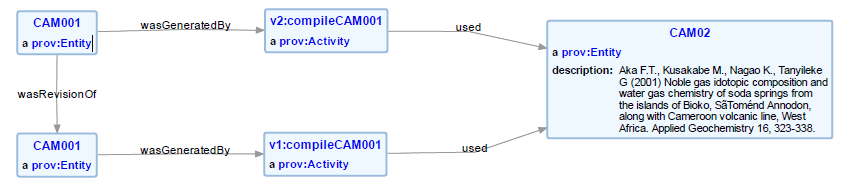
\includegraphics[scale=0.70]{figures/CAM001v1v2.png}
	\caption{Provenance graph for the entry CAM001 entry of the Noble Gas Database.  Other than the labels, the structure of each of the data objects is very much the same.}
	\label{CAM001ProvGraph}
\end{figure}

\section{FORM A MAPPING}

The next step involves formulating a method to determine whether a relationship constitutes an add, invalidate, or modify mapping.
An attribute needs to be identified, which can used as a unique identifier for a piece of datum within the dataset.
In tabular data, this would correspond to the row and column of the datum.
However, new entries into a table rarely takes the form of an individual cell.
Entire rows or columns are usually added as a group.
As a result, when adding or invalidating data
This step largely comes fairly easily to data producers since they have a more comprehensive understanding of the actions taken to create the alternate version.
The key comes down to using the proper attribute identifier.
In a tabular context, this often means using the row or column number, but rows and columns are often rearranged.
Adding or removing a column would 

In the case of the copper minerals dataset, each mineral had a unique name which was used to determine if an entry was removed or added to the dataset.
All names from one version was placed into a set, and all the names of the next version were placed into another set.

So basically, what we do is we figure out what attributes will identify the entries in the data.
Then we compare these sets of attributes to determine if they only exist in one version or both.
The model then tells us how to link together the objects.

For copper

\section{GENERATE VERSIONING GRAPH}

An encoding can now be generated after a method of mapping has been determined.
In current practice, the method of publishing version information comes in the form of a change log.
In this application, the data is published as a versioning graph, leveraging the structure of the concept model.
This allows the data to be stored into a triple store and then retrieved through queries.
In addition, change log and linked data technologies can be combined together into a hybrid artifact using different encoding schemes that embed linked data graphs into documents.
Execution of these hybrid logs had mixed results as very large graphs with many changes became very difficult to load.
As optimization methods are outside the scope of this application, efficiently merging versioning graphs into change logs is not pursued further.
However, in change logs, changes are presented in sections by type.
As a result, when generating the triples, the changes are collected and organized first, then output.

A selection of triples have been extracted from the larger Noble Gas versioning graph in Figure \ref{NobleGraph1}, demonstrating how entries appear.
The graph reads, EGY001 was added, ANC001 no longer appears, and column 11 of CAM001 underwent a modification.
In the case of Figure \ref{NobleGraph1} and \ref{CopperGraphVerGraph}, the graph was extracted from linked data embedded into a change log.
As a result of limitations in the encoding, a unique attribute combining the column number and the row identifier was used to identify the column attribute.
The decision to combine them was to produce an easier graph to run a flow computation on.
An alternative construction would be to use just the column identifier and share it with other entries.
This results in the graph more similar to Figure \ref{NobleGraph2} where column 11 links to multiple changes.

\begin{figure}
	\centering
	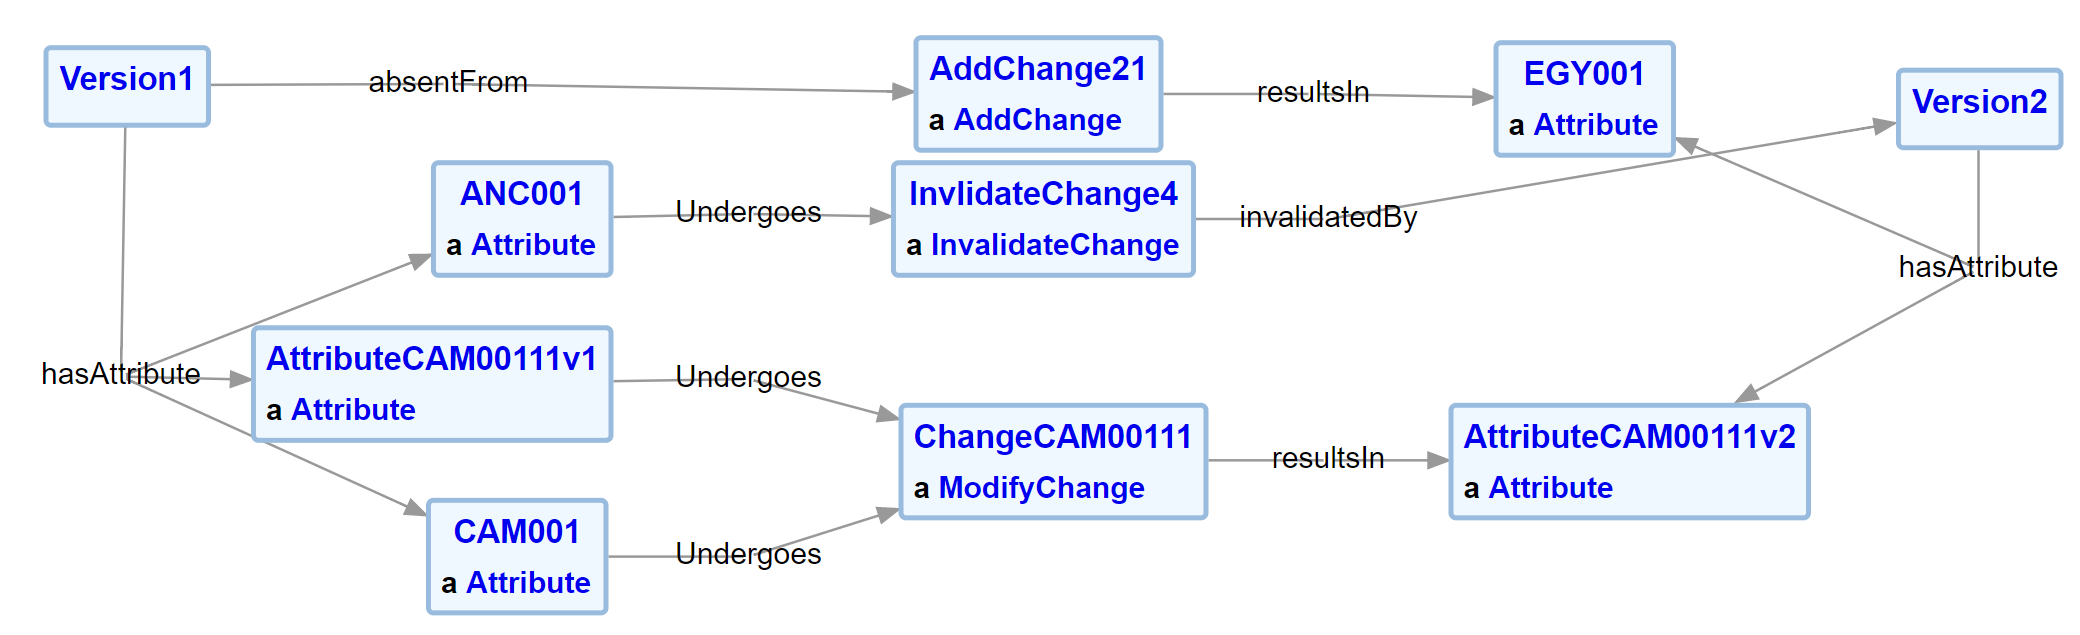
\includegraphics[scale=0.30]{figures/NobleVersion.png}
	\caption{Some initial entries from versions 1 and 2 of the Noble Gas dataset}
	\label{NobleGraph1}
\end{figure}

\begin{figure}
	\centering
	\begin{adjustbox}{addcode={\begin{minipage}{\width}}{
					\caption{Versioning Graph representing the linked data graph with selected entries of additions, invalidations, and modifications. 
			}\end{minipage}},rotate=90,center}
		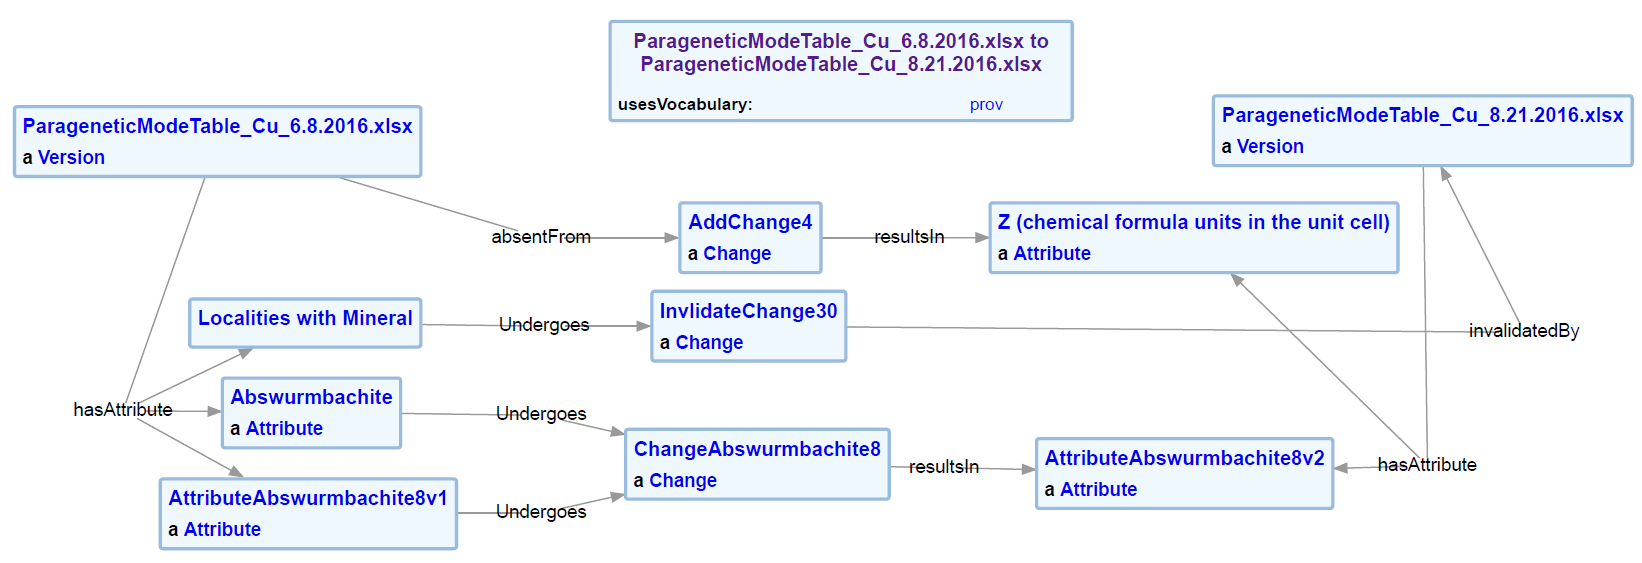
\includegraphics[scale=0.5]{figures/VersioningGraph2.png}%
	\end{adjustbox}
	\label{CopperGraphVerGraph}
\end{figure}

\section{MULTIPLE LINKED VERSIONS}

Versions do not always appear in pairs.
While the figures in this document so far have depicted a comparison between only two versions, versioning often involves more than two objects, either in sequence or parallel.
Using the construction outlined in the previous three sections, many changes can be compiled together into a graph in a changelog.
After all additions, invalidations, and modifications have been compiled into a single graph, a complete mapping from version one to version two may be developed.
The orientation of the relationships in the graph allows a flow to be created from attributes in version one to corresponding attributes in version two.
Taking version two and performing the same graph construction to a version three results in not only a flow from version two to version three, but also from version one to version three.
As a result, the flow can be used to construct a mapping from version one to version three or any future version.

\begin{figure}
	\centering
	\begin{adjustbox}{addcode={\begin{minipage}{\width}}{
					\caption{Versioning Graph representing the linked data graph with selected entries of additions, invalidations, and modifications after the publication of the third version. 
			}\end{minipage}},rotate=90,center}
		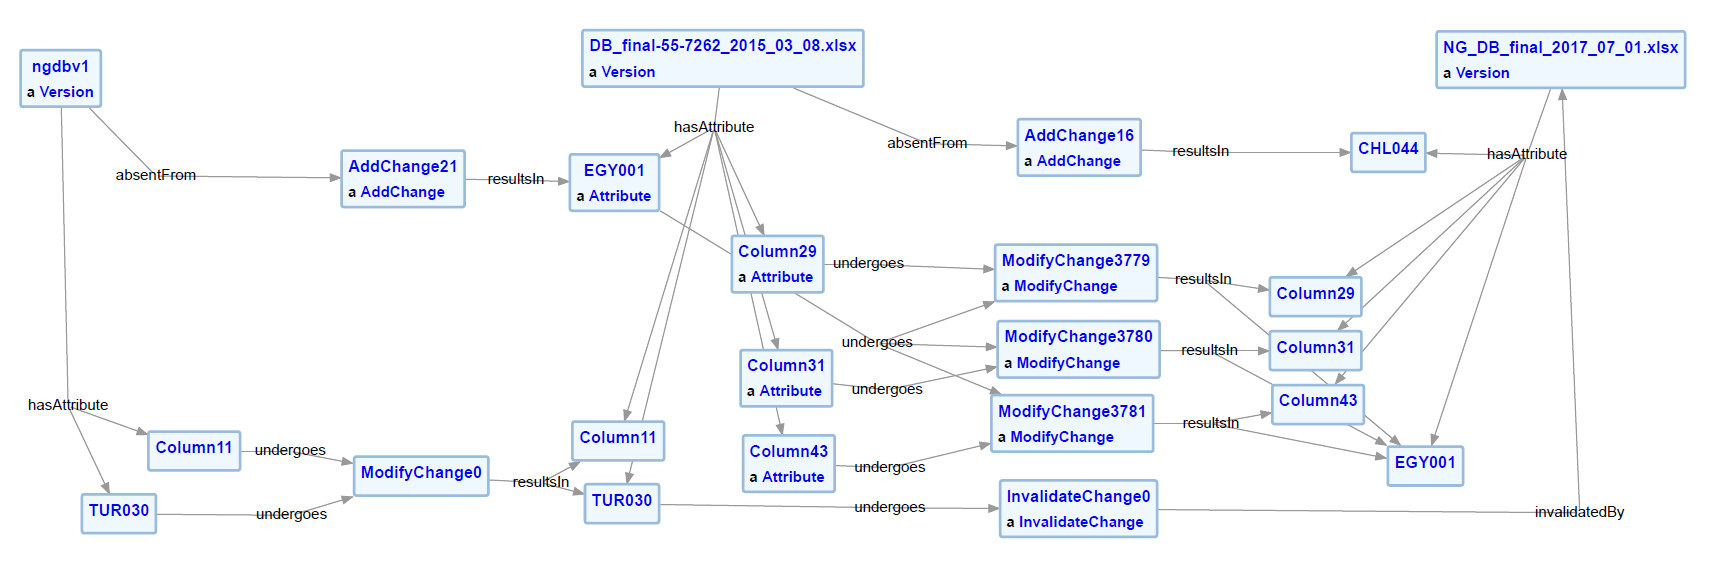
\includegraphics[scale=0.5]{figures/NobleVersion2.png}%
	\end{adjustbox}
	\label{NobleGraph2}
\end{figure} % Version Graph
%%%%%%%%%%%%%%%%%%%%%%%%%%%%%%%%%%%%%%%%%%%%%%%%%%%%%%%%%%%%%%%%%%%
%                                                                 %
%                            CHAPTER FIVE                         %
%                                                                 %
%%%%%%%%%%%%%%%%%%%%%%%%%%%%%%%%%%%%%%%%%%%%%%%%%%%%%%%%%%%%%%%%%%%

\chapter{Data Volatility}

\section{Introduction}

Capturing change counts is important but understanding how a data set changes over time is also valuable to users.

Look at Figure \ref{GCMDC1} and notice the different total amounts of change in each version of GCMD Keywords.
The group appears to do significantly less work in updating the data set after Version 8.1, but the appearance only occurs because the versions are disconnected from time.
Once we're able to quantify change, we can begin looking at trends over time.
Data volatility is the likelihood or rate of data change.
Volatility helps explain the 
We want to know if data versions are hiding the actual rate of change

\section{Determining Volatility}

Instead of charting the version changes in evenly wide bars, the versions are spread across time based on the time of publication to the KMS as seen in Figure \ref{GCMDPlot1}.
\begin{figure}%[b]
	\centering
	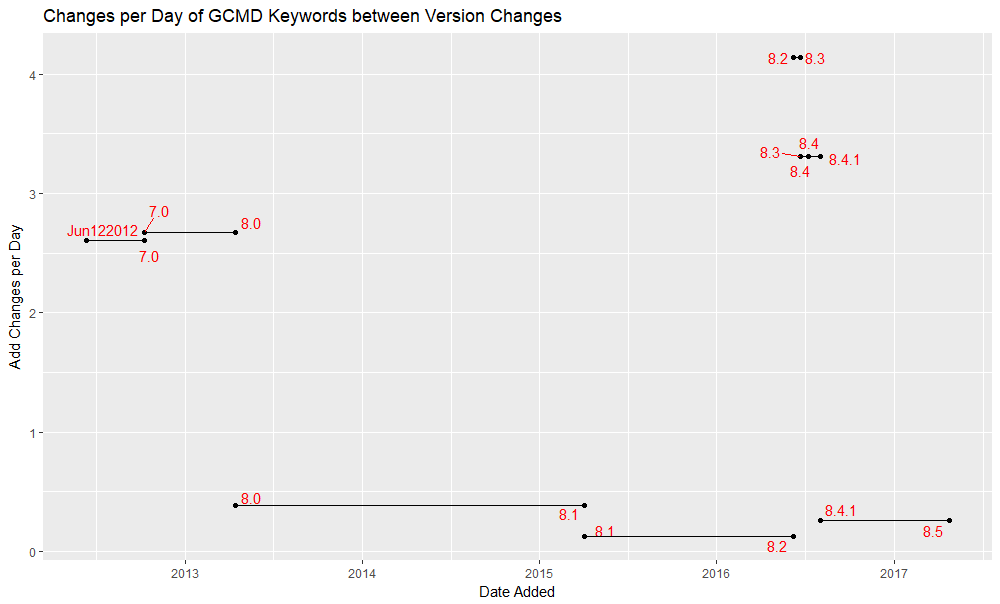
\includegraphics[scale=0.56]{figures/GCMDPlot1.png}
	\caption[Global Change Master Direcotry counts distributed over time.]{Add counts for all versions of GCMD up to 8.5 evenly distributed over the time of version validity.}
	\label{GCMDPlot1}
\end{figure}
Since each of the versions were dominated by the \textbf{Add} counts, the count is divided by the number of days between the publication of a version on the left side of the line and the release of the replacement version on the right side of the line.
The height of the line on the chart gives the steady rate of change until the release of the new version.
The area underneath the line is the total amount of change the new version introduces.
Since each version packages together all the changes into a single release, the actual change rate is unknown.

Three observable clusters appear in the time aware presentation of the versions, highlighted in Figure \ref{GCMDPlot1Cluster}.
\begin{figure}%[b]
	\centering
	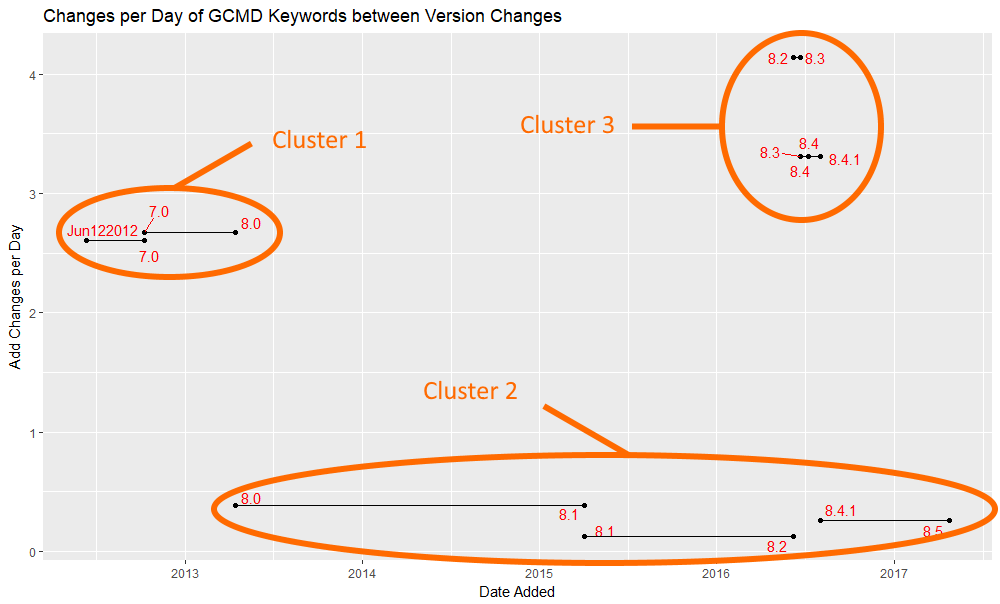
\includegraphics[scale=0.56]{figures/GCMDPlot1_Cluster.png}
	\caption[Global Change Master Directory count distributed over time with clusters marked.]{The change rate of different versions organize into three visible clusters. Cluster 2 denotes a sudden burst of version releases which is notable.}
	\label{GCMDPlot1Cluster}
\end{figure}
According to the Keyword Governance and Community Guide Document \cite{gcmd_gov}, ``Full GCMD keywords list releases get a new major version number (e.g., 8.0). Incremental releases for updates to topics, terms, and variables get a new minor version number (e.g., 8.1).”
The statement explains the activity in Cluster 1 where there are sufficient changes to warrant a full release of the keywords.
Cluster 2 captures the change rate and duration of minor versions, except those from 8.2 to 8.4.1 which are in Cluster 3.
Cluster 3 demonstrates a flurry of activity occurring between June 7, 2016, to August 2, 2016.
Considering the previous pattern of taking at least six months between releases, three minor version releases within as many months is highly unusual.

An immediate concern is that Cluster 3 does not result from a sudden burst of activity, necessitating rapid version replacement.
An inquiry into reasoning behind the successive publication returned a statement that the government customer had requested the action.
Another way to dig into the behavior is to look into the impact assessments accompanying the versions.
Impact assessments prior to Version 8.5 are not publicly available, and only assessments for versions 8.2, 8.3, and 8.4 were received upon request.
Of the 6 requests affecting Earth Science Keywords in 8.2, published June 7, 2016, 4 were made in 2014, and the remaining 2 were made in 2015.
Version 8.3 had 8 entries in its impact assessment with 7 entries originating in 2014, and the remaining entry from 2015.
The 6 entries 8.4’s impact assessment has 5 entries from 2008 and 1 entry from 2015.
The data is collected in Table \ref{table:GCMD_old}.
\begin{table}
	\caption{Global Change Master Directory versions with old start time changes.}
	\label{table:GCMD_old}
	\centering
	\begin{tabular}{|c|c|c|c|c|}
		\hline
		Version Name&	Publish Date&	2008&	2014&	2015\\ \hline
		8.2&	June 7, 2016&	0&	4&	2\\
		8.3&	June 21, 2016&	0&	7&	1\\
		8.4&	July 7, 2016&	5&	0&	1\\
		\hline
	\end{tabular}
\end{table}


\section{Earth Observing Laboratory}

The Earth Observing Laboratory (EOL) of the National Center for Atmospheric Research (NCAR) distributes small data sets, around 10-12 files per data set, regarding lower atmospheric data beginning in 2005 \cite{EOL}.
The EOL data sets are somewhat unique in the data set size means management often does not require automation.
In mid-2014, EOL began assigning versions to stored data sets.
When receiving a new version of a data set from a researcher, the practice is to upload the entire new data set, and replace all old files.

Of the 1335 data sets maintained by EOL with versions, only 180 data sets had more than one version.  
The full distribution of version counts is in Table \ref{table:EOL_Versions}
\begin{table}
	\caption{Version Content of Earth Observing Laboratory Data Sets}
	\label{table:EOL_Versions}
	\centering
	\begin{tabular}{|c|c|}
		\hline
		Number of Versions& Number of Data Sets\\ \hline
		1&	1155\\
		2&	141\\
		3&	26\\
		4&	10\\
		5&	3\\
		Total&	1335\\
		\hline
	\end{tabular}
\end{table}
The 1155 other data sets were filtered out since change counts could not be computed for single-version collections.
Since all the files are replaced on an update and a unique file identifier like a hash sum was unavailable, file matching between versions rely on filenames to perform change mappings.
For all files that matched names across versions, the relation was classified as \textbf{Modify}.  
The approach will over-count the number of modifications, but provides an upper bound on the data set volatility in the repository.  
Each count is then normalized by the number of files in the previous version to standardize comparison between data sets regardless of data set size.  
The average for each data set is taken for each change type.

\section{EOL Versioning Behavior}

Given that EOL replaces the entire old data set when updating, the expected behavior of the transitions would be \textbf{Modifies} concentrating close to 1 and \textbf{Adds} and \textbf{Invalidates} distributed close to 0.
The assumption is that researchers have little reason to change the file naming scheme.
The data surprisingly indicates that data sets in EOL primarily gravitate towards \textbf{Addition} and \textbf{Invalidation} values of 1.
\textbf{Modify} counts score more close to 0 in a complete reversal of expectations.

Figure \ref{EOL_Adds} shows the distribution of \textbf{Add} scores.
\begin{figure}%[b]
	\centering
	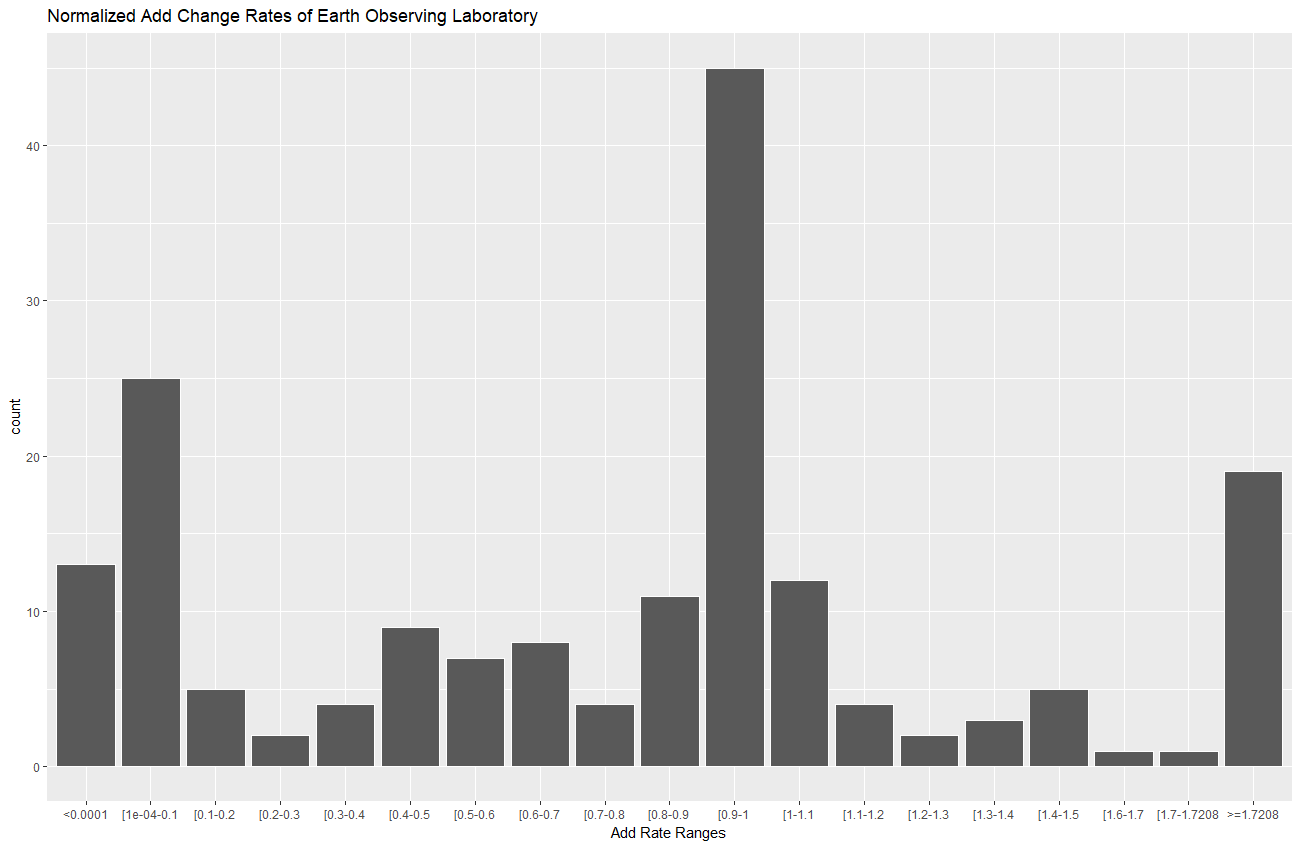
\includegraphics[scale=.43]{figures/Eol_Adds.png}
	\caption{Distribution of average normalized Add counts for each data set in Eath Observing Laboratory.}
	\label{EOL_Adds}
\end{figure}
The primary feature of the chart is the bar situated in the `[0.9-1' range, meaning that about 45 data sets add a number of files equal to the original size of the data set.
Secondary features include the bars on the far right and far left of the chart, but the bar on the right side is a collection of outliers.
In the outlier data sets, the size of the data set increased drastically compared to the behavior of other data sets managed by EOL.
Outliers are determined by collecting values above 1.5 times the interquartile range (IQR) showing in Table \ref{table:EOL_Change}.
\begin{table}
	\caption{Normalized Change Statistics}
	\label{table:EOL_Change}
	\centering
	\begin{tabular}{|c|c|c|c|}
		\hline
		Stat&	Add&	Invalidate&	Modify\\ \hline
		Mean&	0.714312707&	0.654819294&	0.345180706\\
		Std. Dev&	0.509878564&	0.420093557&	0.420093557\\
		Min&	0&	0&	0\\
		Q1&	0.28635075&	0.142857&	0\\
		Med&	0.9146635&	0.9642855&	0.0357145\\
		Q3&	1.00358625&	1&	0.857143\\
		Max&	54.25&	1&	1\\
		IQR&	0.7172355&	0.857143&	0.857143\\
		\hline
	\end{tabular}
\end{table}
A more muted distribution appears around the 0.5 mark where data sets grow more gradually.

The normalized \textbf{Invalidation} score in Figure \ref{EOL_Invs} shows a majority of data sets removing all or almost all files in the data set.
\begin{figure}%[b]
	\centering
	\includegraphics[scale=.6]{figures/Eol_Inv.png}
	\caption{Distribution of average normalized Invalidate counts for each data set in Eath Observing Laboratory.}
	\label{EOL_Invs}
\end{figure}
Coupled with the information that a quarter of the data sets added close to the original data sets' size of files suggests that the entire data set is being replaced.
\textbf{Invalidations} do not have outliers since only files within the data set can be removed.
The data is extremely biased with only 0.04 separating the median and maximum value.
From Table \ref{table:EOL_Change}, at least a quarter of values are 1.
Figure \ref{EOL_Invs} also shows a muted distrubtion around 0.5.

Figure \ref{EOL_Mods}, representing the normalized \textbf{Modify} distribution, is almost a mirror of the \textbf{Invalidation} chart.
\begin{figure}%[b]
	\centering
	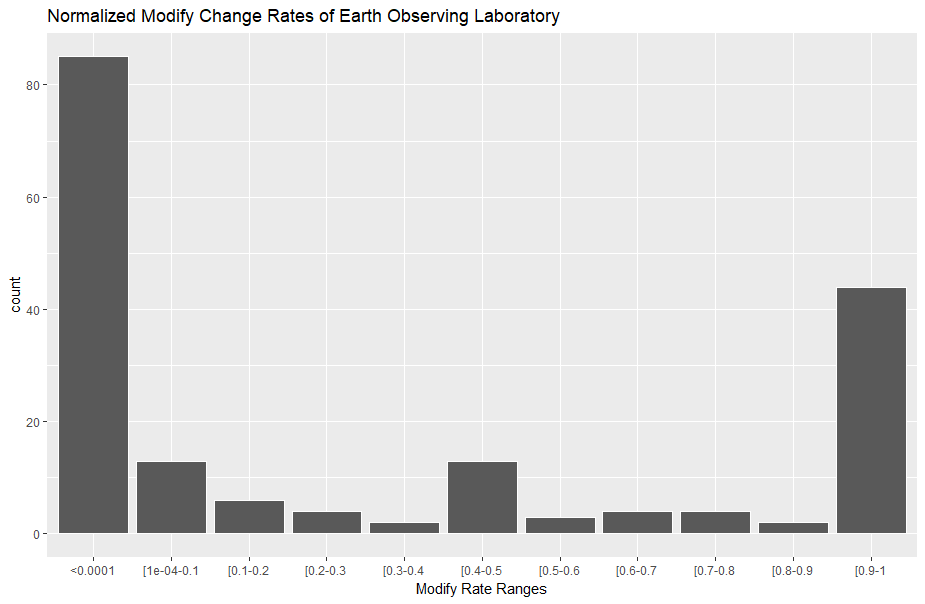
\includegraphics[scale=.6]{figures/Eol_Mod.png}
	\caption{Distribution of average normalized Modify counts of each data set in Eath Observing Laboratory.}
	\label{EOL_Mods}
\end{figure}
The right bar is specifically cut off to capture only 0s, showing that almost a majority of data sets modify 0 files, having 0 files that share names between versions.
The distribution is consistent with a practice of removing all the files in a data set and replacing the files with a new data set using different filenames.
The second feature of this graph shows around 40 data sets in which all or almost all files match across versions.
A small spike of data sets are centralized around 0.5, very much like the other normalized change graphs.

The high concentration of data sets towards 1 in \textbf{additions} and \textbf{invalidations} suggests a more complicated interaction within the data sets.
Individually, the normalized distributions do not show the connection between all three changes since the changes share a common feature, the version transition the changes describe.
Together, the AIM changes create a coordinate in three dimensional space, showing the inter-relation of the changes. 
Figure \ref{EOL_AIM} shows a scatter plot grouping unnormalized change counts for each version.
\begin{figure}%[b]
	\centering
	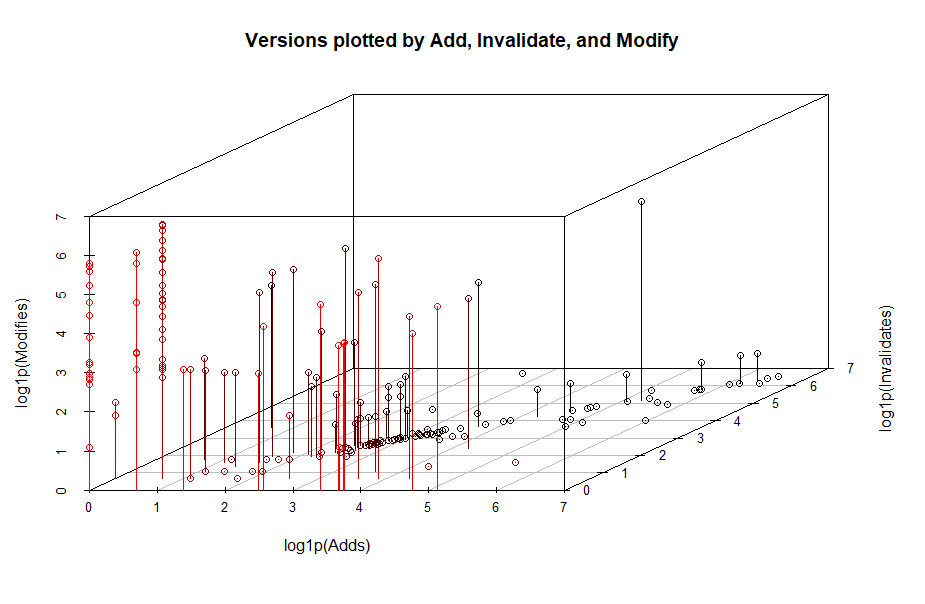
\includegraphics[scale=.6]{figures/Eol_Versions_3d.png}
	\caption{Distribution of average normalized Modify counts of each data set in Eath Observing Laboratory.}
	\label{EOL_AIM}
\end{figure}
Unlike the other charts, the size of the changes are not normalized by data set size, but the values have the log1p function applied to account for a heavy bias towards 12 and 13.
Notice the one-to-one trend between \textbf{Adds} and \textbf{Invalidates} which shows the tendency of data sets to replace every file and assign a new filename.
If the two changes did not co-occur, a normalized \textbf{Add} score of 1 would indicate that data sets tend to double in size instead.
The files are more likely to retain filenames when only a few files in a data set are being modified.

\section{Analysis}

\subsection{Impact Assessment Change Counts}
\begin{table}
	\caption{Differences in VersOn and Impact Assessment metrics}
	\label{table:GCMD_metric}
	\centering
	\begin{tabular}{|r|r|r|r|}
		\hline
		Version & Add & Invalidate & Modify\\ \hline
		8.2(VO)&	53&	1&	26\\
		-8.2(IA)&	48&	0&	4\\
		\hline
		&	\textbf{5}&	\textbf{1}&	\textbf{22}\\
		\hline
		8.3(VO)&	58&	0&	13\\
		-8.3(IA)&	58&	0&	10\\
		\hline
		&	\textbf{0}&	\textbf{0}&	\textbf{3}\\
		\hline
		8.4(VO)&	53&	0&	1\\
		-8.4(IA)&	66&	0&	5\\
		\hline
		&	\textbf{-13}&	\textbf{0}&	\textbf{-4}\\
		\hline
		8.5(VO)&	68&	2&	22\\
		-8.5(IA)&	55&	0&	30\\
		\hline
		&	\textbf{13}&	\textbf{2}&	\textbf{-8}\\						
		\hline
	\end{tabular}
\end{table}

\subsection{Hidden Volatility}

Each version of a data set stored in EOL is assigned three different times, “version publish time,” “version creation time,” and “version modification time.”  
Version publish time indicates the time the version was made available to the public, usually the data set was added to the database.  
Version creation time denotes the moment at which a version designation was given to the collection of files, beginning in mid-2014 when the versioning system was implemented.  
Version modification time indicates the time at which the version metadata was changed.  
Using version publish time most closely resembles the duration of version validity, and the following computations use version publish time.

Some of the data needed to be filtered out to provide valid results.  
Due to a few coding errors in time assignments, 7 versions had to be removed because the durations were negative.  
Duration is measured in days, and the rate of version publication is determined by taking the inverse of the duration.  
To acquire the AIM change rates, the changes are divided by the associated duration for each version.  
Since the rates are closely concentrated at 0, the log of the rates are taken to give the values a more log-normal distribution.  
Values where an AIM change is 0 had to be removed in order to properly apply the log function.  
The remaining number of entries can be found in Table XX.

Since the durations are not normally distributed, but concentrated close to 0, the log of the durations are taken to normalize the data.  
The log function is also applied to the AIM changes to normalize the data.  
The inverse of the log of the duration is taken to acquire the rate of version release.

The Kolomogorov-Smirnov Test was used to determine if the Adds, Invalidates, or Modifies follow a distribution separate from the version publication distribution.  
A difference indicates that the AIM changes exhibit a behavior apart from the version releases.  
As seen in Figures XX, XX, and XX, the distributions of AIM changes over duration are offset due to a larger magnitude of values per version.  
The change rates were translated by the difference in means between the version mean and the associated change mean after log normalization to make the values valid for comparison by the Kolomogorov-Smirnov test.

\begin{figure}%[b]
	\centering
	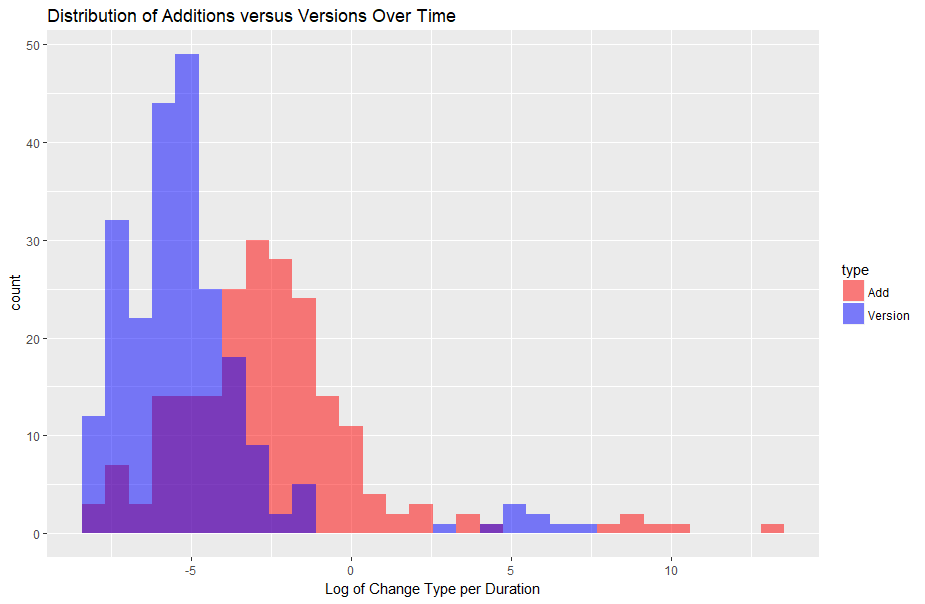
\includegraphics[scale=.6]{figures/Eol_Add_Ver_Rate.png}
	\caption{Distribution of average normalized Modify counts of each data set in Eath Observing Laboratory.}
	\label{EOL_Add_Ver}
\end{figure}

\begin{figure}%[b]
	\centering
	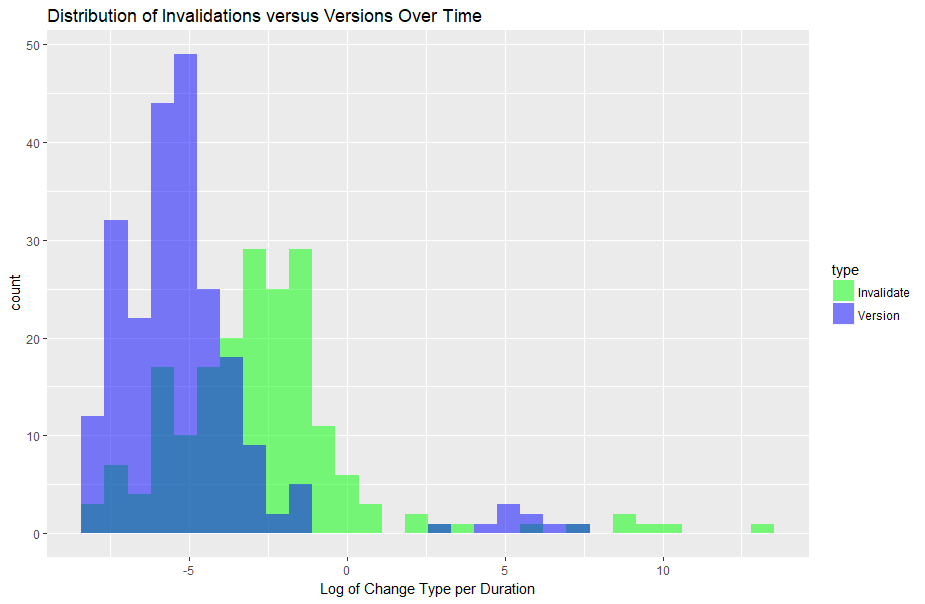
\includegraphics[scale=.6]{figures/Eol_Inv_Ver_Rate.png}
	\caption{Distribution of average normalized Modify counts of each data set in Eath Observing Laboratory.}
	\label{EOL_Inv_Ver}
\end{figure}

\begin{figure}%[b]
	\centering
	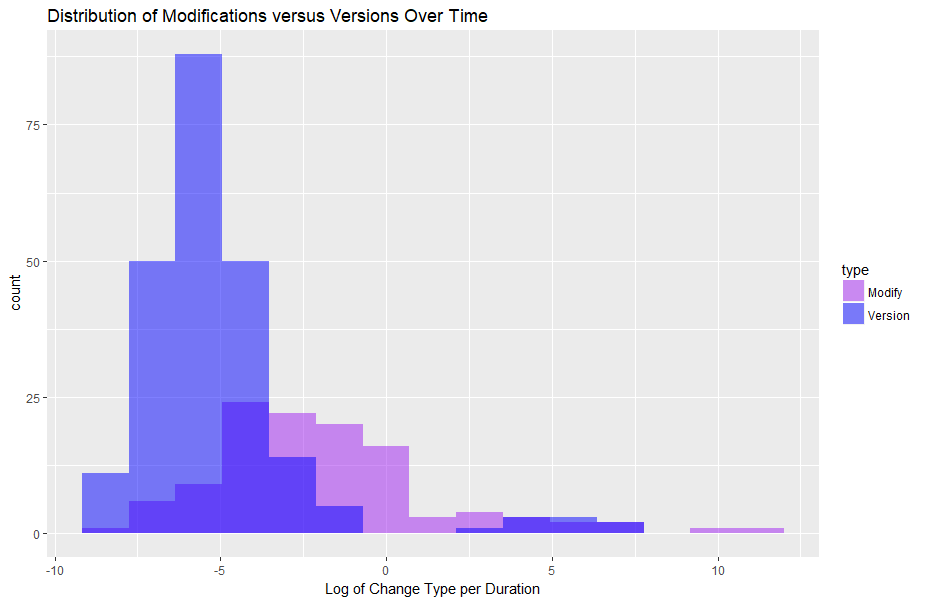
\includegraphics[scale=.6]{figures/Eol_Mod_Ver_Rate.png}
	\caption{Distribution of average normalized Modify counts of each data set in Eath Observing Laboratory.}
	\label{EOL_Mod_Ver}
\end{figure}

\begin{table}
	\caption{Summary of Kolmogorov-Smirnov Test results for Earth Observing Laboratory.}
	\label{table:Eol_KS}
	\centering
	\begin{tabular}{|c|c|c|c|c|}
		\hline
		&	Add&	Invalidate&	Modify&	Versions\\ \hline
		Length&	205&	192&	114&	227\\
		D-Value&	0.12919&	0.14464&	0.19727&	NA\\
		p-Value&	0.05487&	0.02575&	0.005443&	NA\\
		\hline
	\end{tabular}
\end{table}

 % Change Log
%%%%%%%%%%%%%%%%%%%%%%%%%%%%%%%%%%%%%%%%%%%%%%%%%%%%%%%%%%%%%%%%%%%
%                                                                 %
%                            CHAPTER SIX                          %
%                                                                 %
%%%%%%%%%%%%%%%%%%%%%%%%%%%%%%%%%%%%%%%%%%%%%%%%%%%%%%%%%%%%%%%%%%%

\chapter{CHANGE DISTANCE} \label{ch:distance}

\section{Introduction}

Use Case 2 addresses the use of versions to communicate how different two objects are.
Many versioning systems use dot-decimal identifiers to signify whether a change is large, medium, or small.
The exact requirements to determine change size differs widely across different domains and applications.
The versioning graph provides a new, more regular method to quantify change between objects using versioning operations.
The work done with GCMD Keywords shows the qualitative relationship between version identifiers and change distance.
Work with the MBVL data set then extends VersOn to give more detailed accounting with the change capture method.

\section{Utilized Data Sets}

\subsection{GCMD Keywords}

The Global Change Master Directory (GCMD) is a metadata repository used by NASA to store records of its available data sets \cite{Miled:2001:GCM:372202.372324}.
They employ a set of keywords to make NASA Earth Science data sets searchable.
These words tag and label datasets into strictly defined categories \cite{GCMDKey}.
GCMD Keywords do not qualify as a standard web ontology since it does not constitute a class hierarchy.
The management team stored early versions of the keywords in Excel spreadsheets, and a centralized distribution system was not used until June 12, 2012.
The Key Management Service now serves the keywords directly in a variety of formats.
Each version of the keywords, encoded in RDF, were downloaded into separate files.
Only versions from June 12, 2012 and after were available, resulting in 9 version files.
Each keyword corresponds to a unique identifier, and when combined with a web namespace, resolves to a data description of the keyword.
Every identifier can be referred to per version by including the version's number at the web identifier's end, meaning that identifiers are consistent across versions.
The taxonomy uses the concepts \textit{skos:Broader} and \textit{skos:Narrower}, where skos refers to the Simple Knowledge Organization System ontology name space, to form a tree hierarchy \cite{skos}.
The tree's root is the keyword, "Science Keywords."
The data set provides an interesting study case due its long sequence of versions and ready use of linked data technology \cite{Stevens2016}.

\subsection{MBVL Classifications} \label{sec:MBVL}

The Marine Biodiversity Virtual Laboratory (MBVL), based at Woods Hole Oceanographic Institution, provides data and services for the study of marine biology with an integrative approach \cite{mbvl}.
In the application studied, a choice of algorithm and taxonomy pairings must be tested on a known population in order to estimate their performance with an unknown microbial population.
The original sequences belong only to the species listed in Table \ref{species_table}.
The original population's census is not available to the author, and only the list of species are known, forming the first data set in this section.
These sequences are then grouped and classified by a specific taxonomy and algorithm pairing.
The workflow utilizes two taxonomies, the Ribosomal Database Project (RDP) and the Silva taxonomy.
Using these databases, the Species-level IdentificatioN of metaGenOmic amplicons (SPINGO) or the Global Alignment for Sequence Taxonomy (GAST) algorithms assign taxonomic ranks to each sequence.
The process produces four data sets, each using the same grouping identifiers and having the same size in each group.
Since the data sets have the same number of sequences, the primary difference between the data sets are the ranks assigned to each sequence.

\begin{table}
	\caption{List of species in the original population.}
	\label{species_table}
	\centering
	\setlength{\tabcolsep}{2pt}
	\begin{tabular}{|c|c|c|}
		\hline
		Acinetobacter baumannii & Actinomyces odontolyticus & Bacillus cereus \\
		Bacteroides vulgatus & Clostridium beijerinckii & Deinococcus radiodurans \\
		Enterococcus faecalis & Escherichia coli & Helicobacter pylori \\
		Lactobacillus gasseri & Listeria monocytogenes & Neisseria meningitidis\\
		Porphyromonas gingivalis & Propionibacterium acnes & Pseudomonas aeruginosa \\
		Rhodobacter sphaeroides & Staphylococcus aureus & Staphylococcus epidermidis\\
		Streptococcus agalactiae & Streptococcus mutans & Streptococcus pneumoniae \\
		\hline
	\end{tabular}
\end{table}

\section{GCMD}

\subsection{GCMD Versioning Graph}

The Global Change Master Directory establishes the context that each \textbf{manifestation} of their keyword list are related versions.
Since the unique identifier for each keyword remains the same across versions, they can be used to align a mapping across versions.
\textbf{Additions} and \textbf{invalidations} are detected by checking an identifier's presence within both versions.
A \textbf{modification} occurs when a keyword's \textit{skos:Broader} property differs between adjacent versions.
A difference indicates that the word has been moved to a different place within the taxonomy since identifiers do not change across versions and a keyword only has one parent concept.
Changes over consecutive versions can be collected into a single graph using the method in Section \ref{sec:multiver} to chain together versioning graphs.
A change log was generated for each pair of consecutive versions in GCMD Keywords and embedded with JSON-LD.
Versioning graphs for each adjacent version was created by extracting JSON-LD from the corresponding change log, and entering the triples into a Fuseki triple store.

\subsection{Connecting Change Counts to Identifiers}

The \textbf{add}, \textbf{invalidate}, and \textbf{modify} counts for each transition are presented in Figure \ref{GCMDC1}.
The query used to extract the counts is found in Listing \ref{gcmd_list}.
Notice the sharp spike in adds and invalidates when transitioning from version 8.4.1 to 8.5.
The version identifiers indicate that at most a minor or technical change has occurred, but the counts of \textbf{addition} and \textbf{invalidation} changes in this transition is more than triple the counts in either of the previous \textbf{major} transitions.
Not only should a small transition not produce changes of this quantity, but the data set's size is on the order magnitude of the recorded \textbf{invalidates}.
In addition, no \textbf{modifications} are revealed, and even the root node "Science Keywords" has been invalidated.
Further investigation of the root word reveals that the name space for the keywords has changed from HTTP to HTTPS.
To provide context, NASA mandated a transition to secure protocols, and the group changed the name space to ensure the URIs remained resolvable.
Since the identifiers are unique, the new name space means they no longer refer to the same object after the protocol change.
Because the keyword identifiers no longer match, the mapping approach results in the total invalidation of keywords from 8.4.1 and the addition of keywords from 8.5.
The dot decimal identifier for the transition from version 8.4.1 to 8.5 does not match the number of changes in the versioning graph.

\begin{table}
	\caption{Global Change Master Directory Keyword Change Counts}
	\label{table:GCMD_main}
	\centering
	\begin{tabular}{|c|c|c|c|c|}
		\hline
		
		Transition&	Add&	Invalidate&	Modify&	Total\\\hline
		June 12, 2012 to 7.0&	310&	9&	22&	341\\
		7.0 to 8.0&	503&	6&	79&	588\\
		8.0 to 8.1&	277&	28&	22&	327\\
		8.1 to 8.2&	53&	1&	26&	80\\
		8.2 to 8.3&	58&	0&	13&	71\\
		8.3 to 8.4&	53&	0&	1&	54\\
		8.4 to 8.4.1&	86&	13&	8&	107\\
		\hline
	\end{tabular}
\end{table}
\begin{figure}[b]
	\centering
	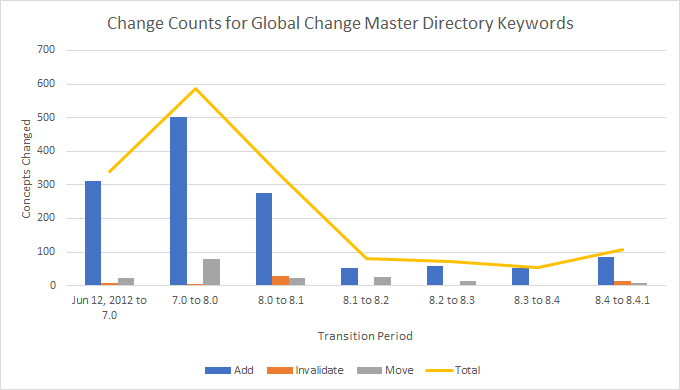
\includegraphics[scale=0.83]{figures/GCMDChartShort.png}
	\caption[Global Change Master Directory Keywords Change counts up to Version 8.4.1]{Add, Invalidate, and Modify counts from the beginning of the Keyword Management System to Version 8.4.1.}
	\label{GCMDC1}
\end{figure}

%\hfill \break
\begin{lstlisting}[language=SPARQL, caption=This query compiles the counts for each subclass of Change in a GCMD versioning graph,label=gcmd_list]
PREFIX vo:<http://orion.tw.rpi.edu/~blee/VersionOntology.owl>
PREFIX rdfs:<http://www.w3.org/2000/01/rdf-schema#>

SELECT ?p (COUNT (DISTINCT ?s) as ?count)
{
?s a ?p .
?p rdfs:subClassOf vo:Change .
} GROUP BY ?p
\end{lstlisting}

Changing the mapping method to account for the new namespace provides a pathway to compare the perceived change by the producer as evidenced by the version identifier with the amount of change in the versioning graph.
To do this, the mapping treats identifiers with HTTP and HTTPS the same. 
Differences in change magnitudes become much clearer after controlling for the altered name space in Figure \ref{GCMDC2}.
All revisions are dominated by \textbf{additions}, but major version changes have counts around 300 to 500 while minor revisions are an order of magnitude smaller.
The transition from version 8.4.1 to 8.5 also seems to follow this trend.
The \textbf{additions} in ``8.4 to 8.4.1" in Figure \ref{GCMDC2} numbers almost a hundred, providing evidence that the trend of decreasing order of magnitudes may now continue as the granularity of the version identifier increases.

\begin{table}
	\caption{Difference in Version 8.5 mapping methods}
	\label{table:GCMD_8_5}
	\centering
	\begin{tabular}{|c|c|c|c|c|}
		\hline
		Mapping Method&	Add&	Invalidate&	Move&	Modify\\ \hline
		Standard&	3097&	3031&	0&	0\\
		Silent&	68&	2&	22&	0\\
		Bridged&	68&	2&	22&	3007\\		
		\hline
	\end{tabular}
\end{table}
\begin{figure}%[b]
	\centering
	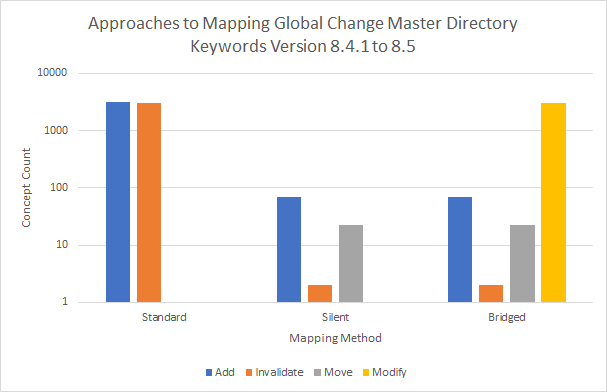
\includegraphics[scale=.9]{figures/GCMD8_5.png}
	\caption{Add, Invalidate, and Modify counts using different methods of mapping identifiers in Global Change Master Directory Keywords Version 8.4.1 to 8.5.}
	\label{GCMDC2}
\end{figure}

\begin{figure}%[b]
	\centering
	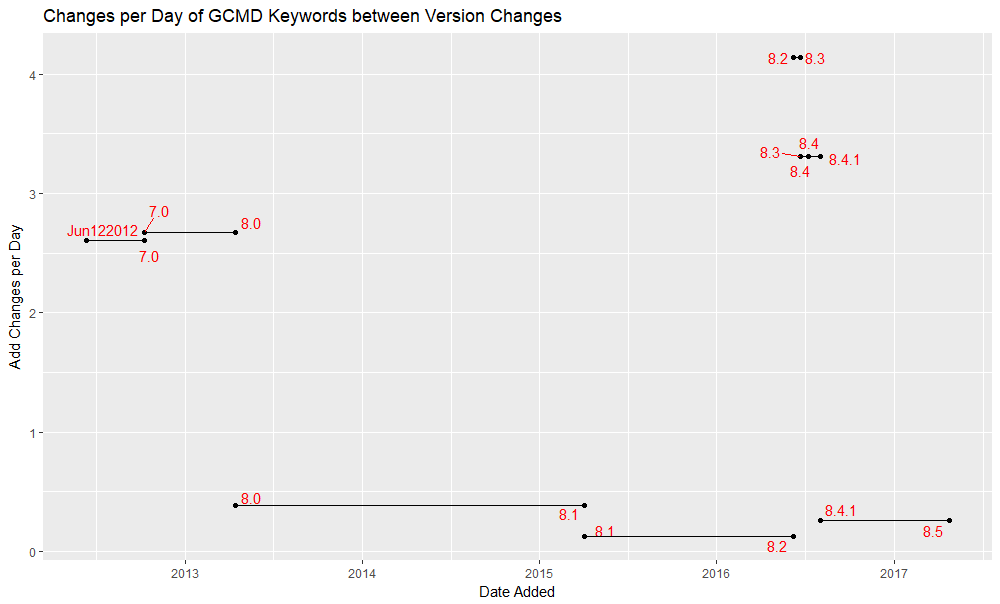
\includegraphics[scale=0.56]{figures/GCMDPlot1.png}
	\caption[Global Change Master Direcotry counts distributed over time.]{Add counts for all versions of GCMD up to 8.5 evenly distributed over the time of version validity.}
	\label{GCMDPlot1}
\end{figure}
\begin{figure}%[b]
	\centering
	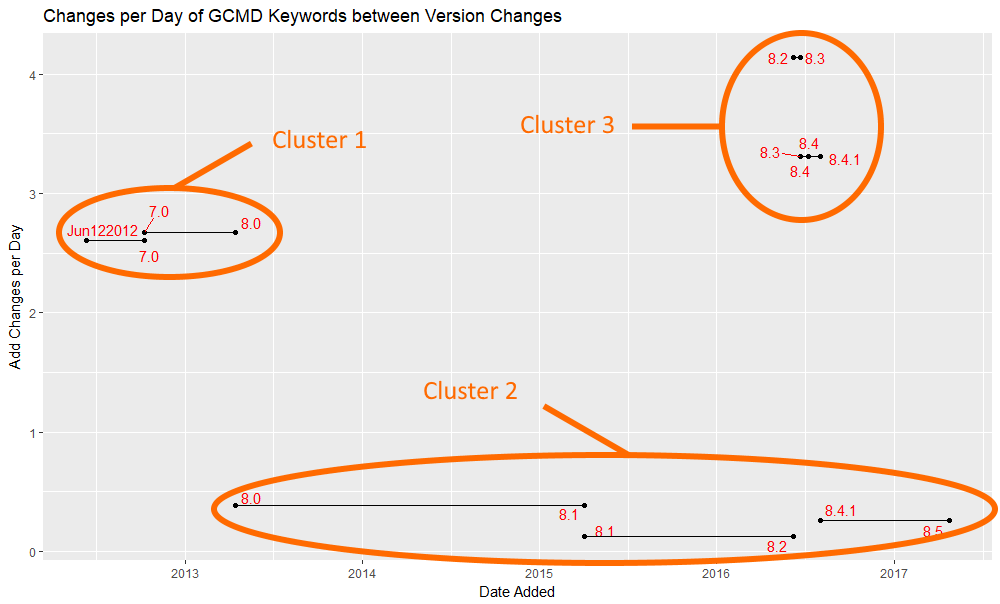
\includegraphics[scale=0.56]{figures/GCMDPlot1_Cluster.png}
	\caption[Global Change Master Directory count distributed over time with clusters marked.]{The change rate of different versions organize into three visible clusters. Cluster 2 denotes a sudden burst of version releases which is notable.}
	\label{GCMDPlot1Cluster}
\end{figure}
\begin{table}
	\caption{Global Change Master Directory versions with old start time changes.}
	\label{table:GCMD_old}
	\centering
	\begin{tabular}{|c|c|c|c|c|}
		\hline
		Version Name&	Publish Date&	2008&	2014&	2015\\ \hline
		8.2&	June 7, 2016&	0&	4&	2\\
		8.3&	June 21, 2016&	0&	7&	1\\
		8.4&	July 7, 2016&	5&	0&	1\\
		\hline
	\end{tabular}
\end{table}

\begin{table}
	\caption{Differences in VersOn and Impact Assessment metrics}
	\label{table:GCMD_metric}
	\centering
	\begin{tabular}{|r|r|r|r|}
		\hline
		Version & Add & Invalidate & Modify\\ \hline
		8.2(VO)&	53&	1&	26\\
		-8.2(IA)&	48&	0&	4\\
		\hline
		&	5&	1&	22\\
		\hline
		8.3(VO)&	58&	0&	13\\
		-8.3(IA)&	58&	0&	10\\
		\hline
		&	0&	0&	3\\
		\hline
		8.4(VO)&	53&	0&	1\\
		-8.4(IA)&	66&	0&	5\\
		\hline
		&	-13&	0&	-4\\
		\hline
		8.5(VO)&	68&	2&	22\\
		-8.5(IA)&	55&	0&	30\\
		\hline
		&	13&	2&	-8\\						
		\hline
	\end{tabular}
\end{table}

\section{MBVL}

\subsection{Variant Versioning Graph}

The experiment conducts activity over two phases in this procedure.
The first phase takes sequences from the original known population and feeds the sequences though a particular algorithm/taxonomy combination to produce a candidate classification.
Since the classifications for the known population sequences is unavailable, there is not sufficient context to perform a valid comparison with the candidate classifications.
The second phase compares the performances of each candidate classification of a algorithm/taxonomy pair.
The use of \textbf{add}, \textbf{invalidate}, and \textbf{modify} varies slightly in this application since all the results use the same sequences.
A versioning graph utilizing just the sequence identifiers would only result in \textbf{modify} changes when taxonomic ranks differ since the sequence identifier exists in both data sets.
The mapping instead uses the sequence identifiers to align comparisons and then the taxonomic rank classification to determine the kind of change.
If the right-hand result specifies more taxonomic ranks, the relationship is an \textbf{addition}.
If the left-hand result is more specific, then the relationship is classified as an \textbf{invalidation}.
If both results have the same precision but the name differs, then the link is a \textbf{modification}.
Otherwise, no change is detected.

Figure \ref{mbvl_chart} shows the changes detected when varying either the taxonomy or the classification algorithm.
\begin{figure}
	\centering
	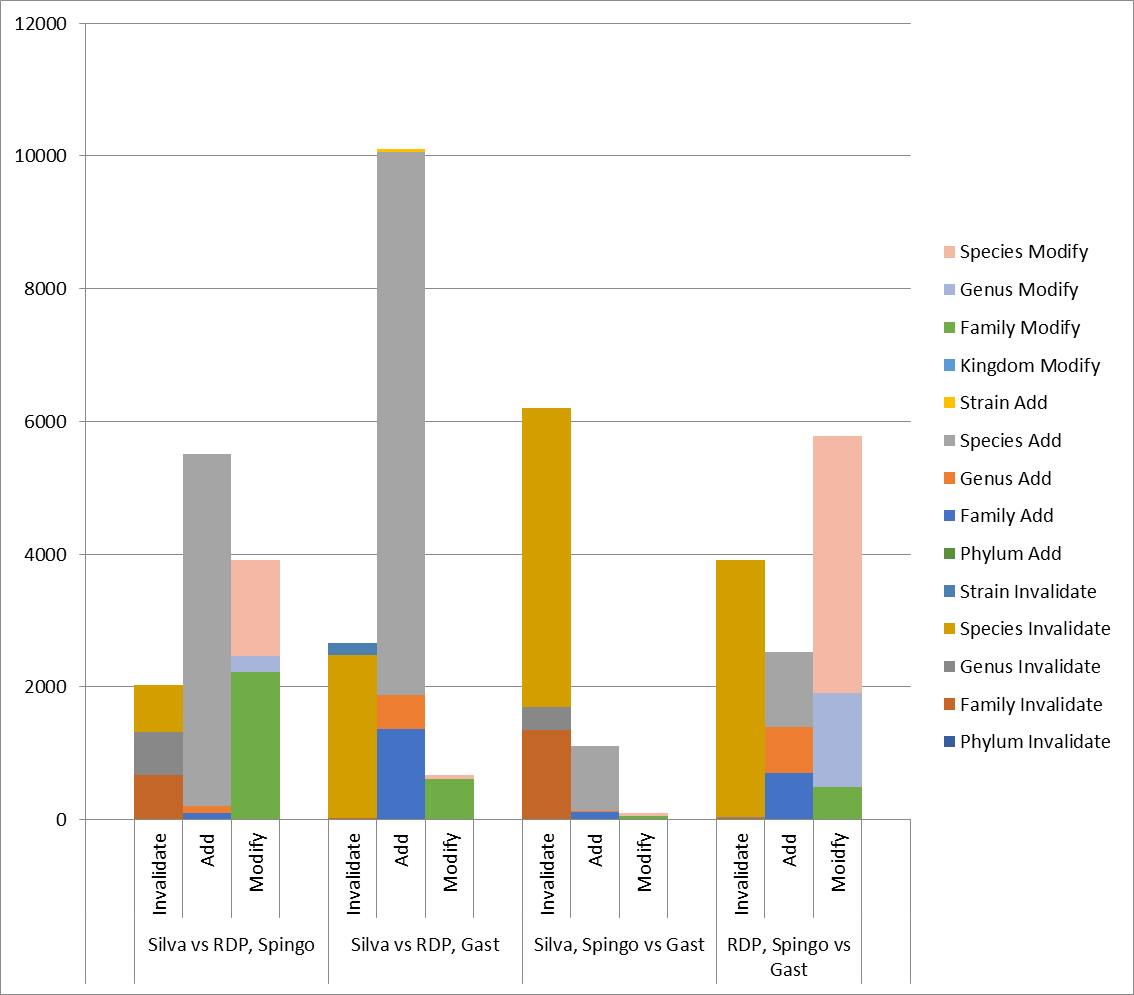
\includegraphics[scale=0.75]{figures/mbvl_chart.png}
	\caption{Compiled counts of \textbf{adds}, \textbf{invalidates}, and \textbf{modifies} grouped by taxonomic rank across algorithm and taxonomy combinations.}
	\label{mbvl_chart}
\end{figure}
No comparison was conducted with different taxonomy and classifier since that would introduce too many sources of variability to differing results in a classification.
Each bar indicates the total number of differences between sequences for a specific kind of change.
The bars are further broken down by the taxonomic rank at which the difference occurred.
For example, in ``Silva vs RDP, Gast", a notable number of classifications differed at the species rank.
The graph also indicates that using the RDP taxonomy often produces more precise classifications since both ``Silva vs RDP, Spingo" and ``Silva vs RDP, Gast" feature a larger number of \textbf{additions} than any other change.
The classifier comparisons feature a high number of \textbf{invalidations}; however, ``RDP, Spingo vs Gast" also displays a higher number of \textbf{modifications} than \textbf{invalidations}.

\section{Analysis}

\subsection{Version Identification}

The versioning process discovered a discrepancy in the identifier assignment in the GCMD Keywords taxonomy.
The original analysis was intended to determine if dot-decimal identifiers could be predicted using the change counts of the versioning graph.
Version 8.5, however, was named with respect to perceived taxonomy changes and did not consider underlying linked data practice revisions.
The disconnect brings into question the accuracy of all prior names and any relationships observed between identifier and change counts.
Non-matching identifiers would explain how 8.4.1 had more additions than any previous minor change but obtains a third bracket identifier.
After accounting for namespace differences in version 8.5, the change counts is in the tens, resembling tallies of other versions in the same identifier bracket.
Version name assignment based on producer perception and not on more concrete measures is concerning.
An incomplete understanding in the amount of change between two versions can lead to flawed expectations during version migration.

The analysis does not to claim that change counts should be the sole mechanism in determining version identifiers.
The counts, however, can provide a more quantitative method to compare version differences.
In Figure \ref{GCMDC2}, the yellow line indicates the total changes made to the data set, performing a similar function as the major/minor/revision version identifier.
Breaking up the changes into types reveals additions dominate manipulations to the data set.
Addition, invalidation, and modification provides deeper insight into how a data set is changing, but some changes can be more impactful than others which this model does not capture.

\subsection{MBVL Analysis}

In Chapter \ref{ch:distance}, the versioning process was used to compare the performance of different taxonomy and algorithm combinations.
The data set diverges from many of the common understandings of versions since each of the versions are not sequential and are largely independent.
The data set of species names in the initial population would not have produced very meaningful results if applied to the versioning model since it lacked sufficient data to map the other data sets together well.

In Figure \ref{mbvl_chart}, the first set of columns in the Silva taxonomy results are versioned against RDP using the SPINGO algorithm.
The naming reflects the orientation in the versioning graph so Silva forms the left-hand version and RDP would be the right-hand version.
In this comparison, using the RDP taxonomy seems to provide more accurate results, most specifically at the species level.
The taxonomies also disagree fairly often at the species and family ranks.
Switching to the GAST algorithm in the second set of columns, RDP once again demonstrates a noticeably greater accuracy in species classification.
There are also significantly fewer disagreements using the GAST algorithm between the two taxonomies.
Looking at the third set of columns, Silva demonstrates greater accuracy classifications under the SPINGO algorithm than under GAST.
Over four thousand of these entries can be classified to the species level when GAST cannot.
In the fourth set of columns, RDP appears to perform better with SPINGO than GAST.
However, the comparison is dominated by a much larger number of disagreements between almost six thousand entries, primarily at the species rank.
On closer inspection, this disagreement is explained by GAST classifying the species for a number of entries as ``uncultured bacterium".
This analysis presents evidence that using the RDP taxonomy with the SPINGO algorithm will produce the most accurate classification results.

\section{Summary}

The result of testing the second hypothesis is inconclusive.
Initial results suggested that identifier assignment and version change size followed an order scale, major changes numbered in the hundreds while minor changes were associated with tens of adds.
The behavior of version 8.5, however, brings into question how accurate or subjective any of the identifiers may be.
Verifying the accuracy of the change counts becomes invalid without further study using other works.
The version graph method does provide a more nuanced view of the distance measure by dividing the total number of changes into groups by operation.
The observation that invalidations almost equaled addition in an add dominated data set in the 8.4.1 to 8.5 transition provided evidence that the data set was completely deleted and an entirely new one added.

The MBVL data set demonstrates a case where versioning graphs can be used to compare the performance of different taxonomy/algorithm pairings.
The ability derives from sub-classing each of the add, invalidate, and modify changes to give a better perspective where the pairings differed.
This approach of extending the versioning graph adds domain knowledge to the version comparison and helps contextualize the observed differences. % Distance
\include{rpichap4_4} % Volatility
%%%%%%%%%%%%%%%%%%%%%%%%%%%%%%%%%%%%%%%%%%%%%%%%%%%%%%%%%%%%%%%%%%%
%                                                                 %
%                            CHAPTER FIVE                         %
%                                                                 %
%%%%%%%%%%%%%%%%%%%%%%%%%%%%%%%%%%%%%%%%%%%%%%%%%%%%%%%%%%%%%%%%%%%

\chapter{ONTOLOGY AND TAXONOMY VERSIONING}

This chapter extensively uses the GCMD Keywords data set to study methods of determining the extent of change in a data set.
The keywords have a long sequence of versions, allowing trends to be observed over the course of releases.

\section{Creating the Versioning Graph}

The Global Change Master Directory maintains and releases the different versions of their keyword list.
From this, it can be concluded that each edition shares provenance and can be used in the same workflow step.
This conclusion is further justified as each keyword concept uses the same Unique Resource Identifier (URI) across versions.
The identifiers also act as an ideal key in the version mapping.
While additions and invalidations are simple to identify using these keys, modifications are not since a change in their key would result in completely different object.
Instead, the immediately broader concept is looked at.
Each keyword uses the concepts skos:Broader and skos:Narrower, where skos refers to the Simple Knowledge Organization System ontology name space, to form a tree hierarchy with the broadest concept "Science Keywords" forming the root.
A modification would then result if a concept moved to a different place in the hierarchy.
This would result in the removal of a child node from the parent and a different broader concept for the child, meaning two modifications occur.
However, in this project, only the child is recorded since it is the concept that moves around in the hierarchy.
Versioning graphs for each comparison was generated by extracting JSON-LD from the corresponding change log, and entering the triples into a Fuseki triple store.

\section{Quantifying Change}

The GCMD group migrated their keywords into a centralized Keyword Management System (KMS) as of June 12, 2012.
Each subsequent keyword release has been supplied an identifier by the management group and the add, invalidate, and modify counts between each transition are presented in Figure \ref{GCMDC1}.
The query used to extract the counts is found in Listing \ref{gcmd_list}.
Notice the sharp spike in adds and invalidates when transitioning from version 8.4.1 to 8.5.
Not only should a small transition not produce changes of this magnitude, but the data sets size is on the order of the recorded invalidates.
In addition, no modifications are revealed, and even the root node "Science Keywords" has been invalidated.
Further investigation of the root word reveals that the name space for the keywords has changed from HTTP to HTTPS.
Since the identifiers are unique, this means they no longer refer to the same object after the protocol change.
This results in the whole data set being invalidated and a new data set being added.
However, the dot decimal identifier only indicates a minor change, demonstrating a difference between the producer's perceived divergence and the actual change.
To provide context, NASA mandated a transition to secure protocols, and the group changed the named space to ensure the URIs remained resolvable.

\begin{figure}%[b]
	\centering
	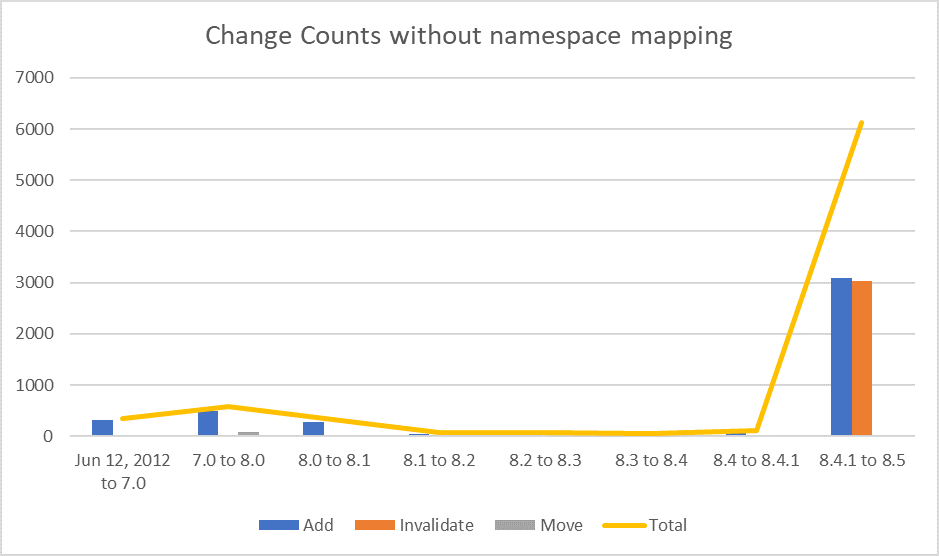
\includegraphics[scale=1]{figures/GCMDChart1.png}
	\caption{Add, Invalidate, and Modify counts in Version 8.5.  The counts show change magnitudes and indicate that major and minor changes differ by orders of magnitude.}
	\label{GCMDC1}
\end{figure}

\hfill \break
\begin{lstlisting}[language=SPARQL, caption=This query compiles the counts for each subclass of Change in a GCMD versioning graph,label=gcmd_list]
PREFIX vo:<http://orion.tw.rpi.edu/~blee/VersionOntology.owl>
PREFIX rdfs:<http://www.w3.org/2000/01/rdf-schema#>

SELECT ?p (COUNT (DISTINCT ?s) as ?count)
{
	?s a ?p .
	?p rdfs:subClassOf vo:Change .
} GROUP BY ?p
\end{lstlisting}

That the data producers did not perceive this change in name space to be a major modification can be demonstrated by accounting for the change and recounting.
In the modified mapping, HTTP and HTTPS identifiers are treated the same.
Differences in change magnitudes become much clearer after controlling for the altered name space in Figure \ref{GCMDC2}.
All revisions are dominated by additions, but major version changes have counts around 300 to 500 while minor revisions are an order of magnitude smaller.
This includes the transition from version 8.4.1 to 8.5.
From the identifier scheme and the change counts, it is clear that the keyword management team expected only minor changes in the keywords.
This analysis demonstrates that relying on data producers to name their versions using the dot decimal identifiers based on their perceived change also relies on their perceiving the intended utilization of their data set by all their users.
The count results seem to indicate that they can differentiate between major and minor revisions, but it also shows that current version labels may not capture all the change within a transition.


\begin{figure}%[b]
	\centering
	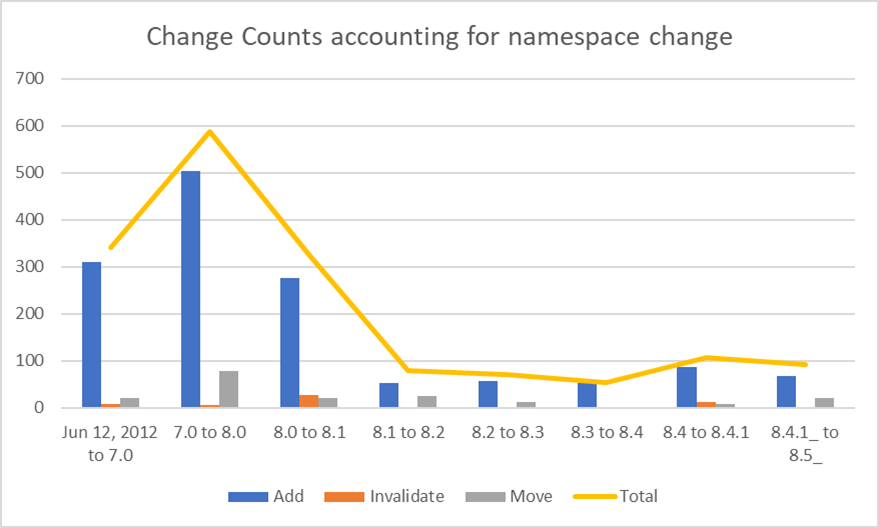
\includegraphics[scale=1]{figures/GCMDChart2.png}
	\caption{Add, Invalidate, and Modify counts ignoring the namespace changes in Version 8.5.  The counts show change magnitudes appropriate for the identifier.}
	\label{GCMDC2}
\end{figure} % Analysis
\chapter{Discussion \& Conclusion}

\section{Hidden Versioning Cost}

\section{Producer/Consumer Versioning Dynamic}

The investigation into GCMD Keywords has demonstrated the importance of investigating beyond sequential version releases.  
The initial hypothesis was that the dominant change count could provide a reliable indicator to differentiate major and minor versions.  
The resulting numbers shows some reflection of the version name in the change counts.  
A more important finding shows that different approaches can be used to evaluate the number of changes in the Version 8.4 to 8.5 transition.  
The difference highlights a barrier between expertise of data producers and consumers within a system.  
Without prior knowledge of the namespace change, the version indicator violates the GCMD Keyword data policy.  
The ability for a consumer to determine the amount of change within a system becomes incredibly important as the associated change document dictates to the data consumer how the producer thinks users should interact with the data.

The GCMD Keyword data set also demonstrates a transparency issue when utilizing a sequential versioning scheme since versions are not bound to a temporal or change count schedule.  
In Figure XX, we can see that there is a sharp drop off in change counts once entering variants of the 8th major release.  
The finding that the change counts do not consistently relate with version identifiers has already been discussed, but the chart is misleading in showing each version equally spaced from the others.  
Temporally, the versions are separated by a variety of durations.  As mentioned in Section XX, the release rate of versions can be artificially controlled, disconnecting the rate of change from time.  
When refactoring time back into the change measurement, we can see very distinct separation in the change rate as well as their conformance with the version identifiers assigned at the end of the change period.  
In particular, we can see in Cluster 2 of Figure XX that versions can be arbitrarily released in quick succession even though work on the changes inside the version began in 2008, 2014, or 2015.  
This finding indicates that version releases cannot be universally trusted to provide a complete picture of the change within a system by itself.

While investigating inconsistencies between change counts found by the change log and those reported by the impact assessment, differences between the metrics became apparent.  
The lack of alignment arose from a difference between the way the community sees and proposes the keywords and the way the keywords are digitally encapsulated and stored in the KMS.  
As a result, the impact assessments do not capture the structural changes that result from additions to the taxonomy.

\section{Hiddent Data Volatility}

The EOL’s small data set size allows it to adopt a comprehensive replacement method.  
The versioning model identified the need for unique file identifiers to determine when files are specifically changed which were not part of the original versioning metadata starting in 2014.  
The process of capturing change within the system using the model naturally led to a set of basic requirements necessary to implement a versioning system.

The 3 dimensional scatter plot in Figure XX shows a very surprising tendency in EOL data sets.  
While the description of update methods suggests data sets should be modify dominant, many of the versions replace and rename all the files in a version.  
The volatility analysis for these versions show that when a version is made it will likely entirely replace the previous version.  
The trend also suggests a concerning behavior of contributing scientists to transition away from a previously established file naming scheme.

The problem with change hiding is that version releases mask a data set’s true volatility.  
From the Kolomogorov-Smirnov test results, each of the change types demonstrated a different distribution from the visible version release rate.


\section{New Versioning Nomenclature}
Analysis of versioned data sets has revealed three types of data, dependent on the way in which versions are released: single, periodic, and intermittent.
Single version data sets contain data which cannot be replicated or in which modification would entirely invalidate the data.
High energy physics, previously mentioned, and surveillance data fit within this category.
The data sets in this category will usually only experience additions and invalidations since scientists cannot change the data.

Periodic data sets exhibit version releases at regular intervals in time.  Large data collections usually exhibit a regular behavior when they follow a periodic data collection scheme.
The ARM data center releases data at daily intervals, meaning new versions every day.
The reasons that ARM data sets are not overloaded with version numbers is that some operations, in this case new files, are masked to increase the pertinence of each version designation.
The problem that masking additions causes is the actual amount of change within the data set over time also becomes masked.
The data set then appears to be intermittent when it actually undergoes periodic changes.  As seen in GCMD Keywords and EOL, changes are not necessarily evenly distributed among versions.  The changes, as a result, are also not evenly distributed across time.  As mentioned with distributed versioning methods, periodic version releases can be used to control the volatility of a data set by collecting many changes over time before publication.  Periodic data sets expend version identifiers very quickly since they must release a version even if few significant changes have occurred.

The final type of data set follows intermittent versioning which is characterized by releasing versions as appropriate or as necessary.  The data sets are not bound by an established release schedules.  In the intermittent category falls GCMD Keywords, the Copper data set, and the Noble Gas data set.  Irregular version releases allows data managers the freedom to reduce the number of versions necessary to manage the data set.  When data managers wait too long to release a new version, the number of changes in a single transition can overwhelm methods to track modifications to the data as seen in the Noble Gas data set.  Since intermittent versions are not released based on time, it is very important that versions are released based on some other quantitative measure of change.  Failing to do so invites unclear or worse arbitrary distinction between versions.  GCMD Keywords define clear requirements for major and minor version releases, but the governance document does not explain the requirements for sub-minor versions which occasionally appear in the keyword repository.

Each data set type can additionally be sub-divided into two categories based on the observations made with the AIM model: Add dominant and Modify dominant.  In the data sets currently studied, none exhibit behavior suggesting an Invalidate dominant data set.  A data set is either Add or Modify dominant when a majority of versions have a majority of either Adds or Modifies.  Add dominance indicates that the data is primarily growing while Modify dominance shows that a data set’s coverage is primarily stable but occasionally undergoes adjustments.  The GCMD Keywords is an example of an Add dominant data set since all its version transitions are comprised of new concepts.  The Noble Gas data set shows modify dominance. % Discussion & Conclusion
%%%%%%%%%%%%%%%%%%%%%%%%%%%%%%%%%%%%%%%%%%%%%%%%%%%%%%%%%%%%%%%%%%%
%                                                                 %
%                            CHAPTER SIX                          %
%                                                                 %
%%%%%%%%%%%%%%%%%%%%%%%%%%%%%%%%%%%%%%%%%%%%%%%%%%%%%%%%%%%%%%%%%%%

\chapter{ONTOLOGY VERSIONING}

Databases already maintain a part of versioning history with a transactional log.
However, they pose an interesting change in context compared to spreadsheets.
Often version comparisons occur between instances of spreadsheet files, but with databases, modifying transactions do not generate a new instance of the database.
Identifying a version would then need to adapt and link transactions to versions.
This can be done through query based citations as described by Proll and Rauber \cite{Proell2013}.
The transaction log also more specifically states the attribute involved, making detection of new attributes into the database more straightforward.
This addresses a particular concern in spreadsheet rows since their attributes have a tendency to be less consistent.
Since RRUFF already possesses an automatically, web accessible change log, the work in this area focuses primarily on deconstructing their code to hook in the concept model with RDFa.

\section{Sea Ice Ontology}

A great many annotations were made to Version 2 of the Sea Ice Ontology.
Maintaining those notes after migration to the new version would provide great value to the project.
From the color code in Table \ref{ColorTable}, yellow and blue changes correspond directly to Modification and Addition transitions, respectively.
In theory, the green concepts would also qualify for a Modify categorization since they would likely have a new URI, meaning that an attribute exists between two versions and something has changed.
However, this would result in a product that is at least the size of the union of the two versions, greatly hindering the scalability of the approach.
The obvious solution would be to leave the attributes unlinked, as in the approach with the spreadsheet application where no change was detected.
The Invalidation change would cover concepts which do not have a mapping into Version 3.
Therefore, the remaining transition types, purple and red require more specific attention than a usual Modify.

\begin{table}
	\newcommand*{\thead}[1]{\multicolumn{1}{|c|}{\bfseries #1}}
	\centering
	\begin{tabular}{ | c | l |}
		\hline
		\textbf{Color} & \thead{Description} \\
		\hline
		Purple & Moved since the previous version of the ontology.\\
		\hline
		Green & Still the same.\\
		\hline
		Yellow & In the same place; but perhaps the name or definition have changed.\\
		\hline
		Red & Suggest changes to be made to both the ontologies and the nomenclature.\\
		\hline
		Blue & New concepts to be added to the ontologies.\\
		\hline
	\end{tabular}
	\label{ColorTable}
	\caption{Color code used by the concept maps made by Ruth Duerr during the planning phase of the Sea Ice Ontology's development.}
\end{table}

 % Future Work
%%%%%%%%%%%%%%%%%%%%%%%%%%%%%%%%%%%%%%%%%%%%%%%%%%%%%%%%%%%%%%%%%%%
%                                                                 %
%                           BIBLIOGRAPHY                          %
%                                                                 %
%%%%%%%%%%%%%%%%%%%%%%%%%%%%%%%%%%%%%%%%%%%%%%%%%%%%%%%%%%%%%%%%%%%

%This method produces a numbered bibliography where the numbers
%correspond to the \cite commands in the text. See the LaTeX manual.
%
\specialhead{REFERENCES}
\begin{singlespace}
\begin{thebibliography}{99}
\bibitem{thisbook} This is the first item in the Bibliography.
Let's make it very long so it takes more than one line.
Let's make it very long so it takes more than one line.
Let's make it very long so it takes more than one line.
Let's make it very long so it takes more than one line.
\bibitem{anotherbook} The second item in the Bibliography.
\bibitem{yetanotherbook} Another item in the Bibliography.
\bibitem{barkstromLibrary}
\bibitem{ATLAS}
\end{thebibliography}
\end{singlespace}

% Note that, if you wish, you can use BibTeX to create your bibliography
% from a database. See section 5.6.2 of Memo RPI.110 for information.
%%% Local Variables:
%%% mode: latex
%%% TeX-master: t
%%% End:
 % bibliography
%%%%%%%%%%%%%%%%%%%%%%%%%%%%%%%%%%%%%%%%%%%%%%%%%%%%%%%%%%%%%%%%%%%
%                                                                 %
%                            APPENDICES                           %
%                                                                 %
%%%%%%%%%%%%%%%%%%%%%%%%%%%%%%%%%%%%%%%%%%%%%%%%%%%%%%%%%%%%%%%%%%%

\appendix    % This command is used only once!
%\addcontentsline{toc}{chapter}{APPENDICES}             %toc entry  or:
\addtocontents{toc}{\parindent0pt\vskip12pt APPENDICES} %toc entry, no page #

\chapter{NOBLE GAS CHANGE LOG GENERATOR VERSION 1 TO 2} \label{app:noble12}
\begin{minted}[linenos, frame=lines, baselinestretch=1.2, breaklines]{python}
from os.path import join, dirname, abspath, isfile
from os import sep as separator
import xlrd, sys, json
import glob
import re


def index_convert(index1):
	if index1 < 17:
		return index1
	elif index1 < 24:
		return index1+1
	elif index1 < 26:
		return 26+(3*(index1-24))
	elif index1 < 28:
		return 44+(3*(index1-26))
	elif index1 < 32:
		return 53+(9*(index1-28))
	elif index1 < 36:
		return 88+(2*(index1-32))
	elif index1 < 38:
		return 95+(4*(index1-36))
	elif index1 < 41:
		return 102+(2*(index1-38))
	elif index1 < 43:
		return 112+(2*(index1-41))
	elif index1 == 43:
		return 172
	elif index1 < 50:
		return 174+(3*(index1-44))
	elif index1 < 54:
		return 191+(index1-50)
	else:
		print 'Error: Out of bounds'
		return -1

def test_alignment():
	for i in range(0, 54):
		print 'version2: {:5} version1: {:5}'.format(i, index_convert(i))

def compare_print(mode, key, val1, val2, v1_file, v1_index = 0, v2_index = 0, changelog = None):
	if changelog:
		if mode == 'r':
			out = u'''        <tr  about="Change{}{}" typeof="vo:ModifyChange">
          <td align="right" rev="vo:Undergoes" resource="v1:Attribute{}{}v1" typeof="vo:Attribute">{:2}({})</td>
          <td property="vo:resultsIn" resource="v2:Attribute{}{}v2" typeof="vo:Attribute">{:2}</td>
          <td>{:>10}</td>
          <td>{:>10}</td>
          <span about="Version1" property="vo:hasAttribute" resource="v1:Attribute{}{}v1"></span>
          <span about="Version2" property="vo:hasAttribute" resource="v2:Attribute{}{}v2"></span>
        </tr>\n'''.format(key, v2_index, key, v1_index, v1_index, v1_file, key, v2_index, v2_index, val1, val2, key, v1_index, key, v2_index)
		elif mode == 'j':
			out = u'''        <tr  id="ModifyChange{}{}">
          <td align="right">{:2}({})</td>
          <td>{:2}</td>
          <td>{:>10}</td>
          <td>{:>10}</td>
          <script type="application/ld+json">\n'''.format(key, v2_index, v1_index, v1_file, v2_index, val1, val2)
		elif mode == 't':
			out = u"{:2}({})\t{:2}\t{:>10}\t{:>10}\n".format(v1_index, v1_file, v2_index, val1, val2)
		elif mode == 'u':
			out = u"""<http://example.com/NG/Version1> vo:hasAttribute <http://example.com/NG/Version1/%s> ;
        vo:hasAttribute <http://example.com/NG/Version1/Column%i> .
<http://example.com/NG/Version1/%s> a vo:Attribute ;
        vo:undergoes <http://example.com/Changelog#ModifyChange%s%i> .
<http://example.com/NG/Version1/Column%i> a vo:Attribute ;
        vo:undergoes <http://example.com/Changelog#ModifyChange%s%i> .
<http://example.com/Changelog#ModifyChange%s%i> a vo:ModifyChange ;
        vo:resultsIn <http://example.com/NG/Version2/%s> ;
        vo:resultsIn <http://example.com/NG/Version2/Column%i> .
<http://example.com/NG/Version2> vo:hasAttribute <http://example.com/NG/Version2/%s> ;
        vo:hasAttribute <http://example.com/NG/Version2/Column%i> .

"""%(key, v1_index, key, key, v2_index, v1_index, key, v2_index, key, v2_index, key, v2_index, key, v2_index)
		changelog.write(out.encode('utf8'))
		if mode == 'j':
			json1 = {
"@context":context,
"@type":"vo:Attribute" ,
"@id":"".join(["http://ngdb.com/v1/Attribute", key, str(v1_index)]) ,
"label":key ,
"undergoes":"".join([host, "ModifyChange", key, str(v2_index)]) ,
"@reverse" :    { "hasAttribute" : "Version1" }
}
			json2 = {
"@context":context,
"@type":"vo:ModifyChange",
"@id":"".join([host, "ModifyChange", key, str(v2_index)]) ,
"resultsIn":"".join(["http://ngdb.com/v2/Attribute", key, str(v2_index)])
}
			json3 = {
"@context":context,
"@type":"vo:Attribute" ,
"@id":"".join(["http://ngdb.com/v2/Attribute", key, str(v2_index)]) ,
"label":key ,
"@reverse" :    { "hasAttribute" : "Version2" }
}
			json.dump([json1, json2, json3], changelog, indent=4, sort_keys=True)
			changelog.write('''
          </script>
        </tr>
''')
	else:
		print '{:5}  version1: {:10} version2: {:10}'.format(key, val1, val2)

labels = {17:"SAMPLING - DEPTH - >,<",
		  25:"[He] - ppm - >,<", 27:"[He] - ppm - err", 28:"[He] - mkcc/ - >,<", 30:"[He] - mkcc/ - err", 31:"[He] - mol/ - >,<", 32:"[He] - mol/ - L H2O", 33:"[He] - mol/ - err",
		  34:"[He+Ne] - ppm - >,<", 35:"[He+Ne] - ppm", 36:"[He+Ne] - ppm - err", 37:"[He+Ne] - mkcc/ - >,<", 38:"[He+Ne] - mkcc/ - g H2O", 39:"[He+Ne] - mkcc/ - err", 40:"[He+Ne] - mol/ - >,<", 41:"[He+Ne] - mol/ - L H2O", 42:"[He+Ne] - mol/ - err",
		  43:"[Ne] - ppm - >,<", 45:"[Ne] - ppm - err", 46:"[Ne] - mkcc/ - >,<", 48:"[Ne] - mkcc/ - err", 49:"[Ne] - mol/ - >,<", 50:"[Ne] - mol/ - L H2O", 51:"[Ne] - mol/ - err",
		  52:"[20Ne] - ppm - >,<", 54:"[20Ne] - ppm - err", 55:"[20Ne] - mkcc/ - >,<", 56:"[20Ne] - mkcc/ - g H2O", 57:"[20Ne] - mkcc/ - err", 58:"[20Ne] - mol/ - >,<", 59:"[20Ne] - mol/ - L H2O", 60:"[20Ne] - mol/ - err",
		  61:"[Ar] - ppm - >,<", 63:"[Ar] - ppm - err", 64:"[Ar] - mkcc/ - >,<", 65:"[Ar] - mkcc/ - g H2O", 66:"[Ar] - mkcc/ - err", 67:"[Ar] - mol/ - >,<", 68:"[Ar] - mol/ - L H2O", 69:"[Ar] - mol/ err",
 		  70:"[Kr] - ppm - >,<", 72:"[Kr] - ppm - err", 73:"[Kr] - mkcc/ - >,<", 74:"[Kr] - mkcc/ - g H2O", 75:"[Kr] - mkcc/ - err", 76:"[Kr] - mol/ - >,<", 77:"[Kr] - mol/ - L H2O", 78:"[Kr] - mol/ err",
		  79:"[Xe] - ppm - >,<", 81:"[Xe] - ppm - err", 82:"[Xe] - mkcc/ - >,<", 83:"[Xe] - mkcc/ - g H2O", 84:"[Xe] - mkcc/ - err", 85:"[Xe] - mol/ - >,<", 86:"[Xe] - mol/ - L H2O", 87:"[Xe] - mol/ err",
		  89:"3He/4He - (R/Ra)me - err", 91:"3He/4He - (R/Ra)corr - err", 93:"3He/4He - Rme - E-8 - err", 96:"3He/4He - Rcorr - E-8 - err", 97:"Rank",
		  98:"He/Ne - >,<", 100:"He/Ne - >,<", 101:"4He/20Ne - >,<", 103:"4He/20Ne - err", 105:"20Ne/22Ne - err", 107:"21Ne/22Ne - (xE-2) - err", 108:"21Ne/20Ne", 109:"21Ne/20Ne - err",
		  110:"22Ne/20Ne", 111:"22Ne/20Ne - err", 113:"38Ar/36Ar - err", 115:"40Ar/36Ar - err", 116:"delta(40Ar)rad", 117:"delta(40Ar)rad - err",
		  118:"He/Ar - He/ - /Ar(air) - >,<", 119:"He/Ar - He/ - /Ar(air)", 120:"He/Ar - He/ - /Ar(air) - err", 121:"He/Ar - 4He/ - /36Ar - >,<", 122:"He/Ar - 4He/ - /36Ar", 123:"He/Ar - 4He/ - /36Ar - err",
		  124:"He/Ar - 4He/ - /40Ar(air) - >,<", 125:"He/Ar - 4He/ - /40Ar(air)", 126:"He/Ar - 4He/ - /40Ar(air) - err",
		  127:"f(He)=(He/Ar)s/(He/Ar)air - >,<", 128:"f(He)=(He/Ar)s/(He/Ar)air", 129:"f(He)=(He/Ar)s/(He/Ar)air - err",
		  130:"Ne/Ar - Ne/ - /Ar(air) - >,<", 131:"Ne/Ar - Ne/ - /Ar(air)", 132:"Ne/Ar - Ne/ - /Ar(air) - err", 133:"Ne/Ar - 20Ne/ - /36Ar - >,<", 134:"Ne/Ar - 20Ne/ - /36Ar", 135:"Ne/Ar - 20Ne/ - /36Ar - err",
		  136:"Ne/Ar - 20Ne/ - /40Ar(air) - >,<", 137:"Ne/Ar - 20Ne/ - /40Ar(air)", 138:"Ne/Ar - 20Ne/ - /40Ar(air) - err", 139:"Ne/Ar - 22Ne/ - /36Ar - >,<", 140:"Ne/Ar - 22Ne/ - /36Ar", 141:"Ne/Ar - 22Ne/ - /36Ar - err",
		  142:"Ne/Ar - 22Ne/ - /40Ar(air) - >,<", 143:"Ne/Ar - 22Ne/ - /40Ar(air)", 144:"Ne/Ar - 22Ne/ - /40Ar(air) - err",
		  145:"f(Ne)=(Ne/Ar)s/(Ne/Ar)air - >,<", 146:"f(Ne)=(Ne/Ar)s/(Ne/Ar)air", 147:"f(Ne)=(Ne/Ar)s/(Ne/Ar)air - err",
		  148:"Kr/Ar - Kr/ - /Ar(air) - >,<", 149:"Kr/Ar - Kr/ - /Ar(air)", 150:"Kr/Ar - Kr/ - /Ar(air) - err", 151:"Kr/Ar - 84Kr/ - /36Ar - >,<", 152:"Kr/Ar - 84Kr/ - /36Ar", 153:"Kr/Ar - 84Kr/ - /36Ar - err",
		  154:"Kr/Ar - 84Kr/ - /40Ar(air) - >,<", 155:"Kr/Ar - 84Kr/ - /40Ar(air)", 156:"Kr/Ar - 84Kr/ - /40Ar(air) - err",
		  157:"f(Kr)=(Kr/Ar)s/(Kr/Ar)air - >,<",158:"f(Kr)=(Kr/Ar)s/(Kr/Ar)air", 159:"f(Kr)=(Kr/Ar)s/(Kr/Ar)air - err",
		  160:"Xe/Ar - Xe/ - /Ar(air) - >,<", 161:"Xe/Ar - Xe/ - /Ar(air)", 162:"Xe/Ar - Xe/ - /Ar(air) - err", 163:"Xe/Ar - 132Xe/ - /36Ar - >,<", 164:"Xe/Ar - 132Xe/ - /36Ar", 165:"Xe/Ar - 132Xe/ - /36Ar - err",
		  166:"Xe/Ar - 132Xe/ - /40Ar(air) - >,<", 167:"Xe/Ar - 132Xe/ - /40Ar(air)", 168:"Xe/Ar - 132Xe/ - /40Ar(air) - err",
		  169:"f(Xe)=(Xe/Ar)s/(Xe/Ar)air - >,<", 170:"f(Xe)=(Xe/Ar)s/(Xe/Ar)air", 171:"f(Xe)=(Xe/Ar)s/(Xe/Ar)air - err",
		  173:"H2 - >,<", 175:"H2 - ppm - err", 176:"O2 - >,<", 178:"O2 - ppm - err", 179:"N2 - >,<", 181:"N2 - ppm - err", 182:"CO2 - >,<", 184:"CO2 - ppm - err", 185:"CH4 - >,<", 187:"CH4 - ppm - err",
		  188:"H2S - >,<", 190:"H2S - ppm - err"}

context = "https://orion.tw.rpi.edu/~blee/provdist/GCMD/VO.jsonld"
host = "http://orion.tw.rpi.edu/~blee/provdist/NobleGas/changelog_json.html#"
#test_alignment()


#print v2_row[0].value
#print indicator_map[v2_row[0].value]

#v1_workbook = xlrd.open_workbook(v1_file)
#v1_sheet = v1_workbook.sheet_by_index(0)
#v1_row = v1_sheet.row(4)

def write_modify(r1, r2, workbook, f_out, mode):
	if mode == 'r':
		out = u'''  <div about="Version1" rel="vo:hasAttribute">
    <div resource="v2:%s" typeof="vo:Attribute">
      <span style="font-weight:bold" property="http://www.w3.org/2000/01/rdf-schema#label">%s</span>
      <table rel="vo:Undergoes">
'''%(r2[0].value, r2[0].value)
	elif mode == 'j':
		out = u'''
    <div about="v2:%s">
      <span style="font-weight:bold" property="http://www.w3.org/2000/01/rdf-schema#label">%s</span>
      <table>
'''%(r2[0].value, r2[0].value)
	elif mode == 't':
		out = u"%s\n"%(r2[0].value)
	elif mode == 'u':
		out = u""

	if mode == 'r' or mode == 'j':
		out = out+'''        <tr>
          <th>Column v1</th>
          <th>Column v2</th>
          <th>Version 1</th>
          <th>Version 2</th>
        </tr>\n'''
	elif mode == 't':
		out = out+"Column v1\tColumn v2\tVersion 1\tVersion 2\n"
	f_out.write(out.encode('utf8'))
		#print '# Searching...'
		#print '# Comparing...'
	for i in range(0,54):
		if r2[i].value != r1[index_convert(i)].value:
			#compare_print(j, v1_row[index_convert(j)].value, v2_row[j].value)
			compare_print(mode, r2[0].value, r1[index_convert(i)].value, r2[i].value, workbook.split('/')[-1], index_convert(i), i, f_out)
	if mode == 'r' or mode == 'j':
		f_out.write('  </table></div><br>\n')
	elif mode == 't' or mode == 'u':
		f_out.write("\n")

def write_removed(v2, col, row, f_out, mode):
	if mode == 'r' or mode == 'j':
		f_out.write('''
      <h3>Columns invalidated by %s</h3>
      <table about="Version2">
'''%(v2.split('/')[-1]))
	elif mode == 't':
		f_out.write("\nColumns invalidated by %s\n"%(v2.split('/')[-1]))

	print "Removed Column"
	for i in col:
        	v1_value = labels.get(i, "")
		if mode == 'r':
			out = u'''        <tr resource="InvlidateChange%i" rev="vo:invalidatedBy" typeof="vo:InvalidateChange">
		<td resource="Attribute%i" rev="vo:Undergoes" typeof="vo:Attribute">%i</td>
          <td about="Attribute%i" property="http://www.w3.org/2000/01/rdf-schema#label">%s</td>
          <span about="Version1" property="vo:hasAttribute" resource="Attribute%i"/>
        </tr>
'''%(i, i, i, i, v1_value, i)
		elif mode == 'j':
			out = u'''        <tr id="InvlidateChange%i" about="InvlidateChange%i">
          <td>%i</td>
          <td>%s</td>
          <script type="application/ld+json">
'''%(i, i, i, v1_value)
		elif mode == 't':
			out = u"%i\t%s\n"%(i, v1_value)
		elif mode == 'u':
			out = u"""<http://example.com/NG/Version1> vo:hasAttribute <http://example.com/NG/Version1/Column%s> .
<http://example.com/NG/Version1/%s> vo:undergoes <http://example.com/Changelog#InvalidateChange%i> .
<http://example.com/Changelog#InvalidateChange%i> a vo:InvalidateChange ;
	vo:invalidatedBy <http://example.com/NG/Version2> .

"""%(i, i, i, i)
		f_out.write(out.encode('utf8'))
		if mode == 'j':
			json1 = {
"@context":context,
"@type":"vo:Attribute" ,
"@id":"".join(["http://ngdb.com/v1/Attribute", str(i)]) ,
"label": v1_value,
"undergoes":"".join([host, "InvalidateChange", str(i)]) ,
"@reverse" :    { "hasAttribute" : "Version1" }
}
			json2 = {
"@context":context,
"@type":"vo:InvalidateChange" ,
"@id": "".join([host, "InvalidateChange", str(i)]) ,
"invalidatedBy"  :   "Version2"
}
			json.dump([json1, json2], f_out, indent=4, sort_keys=True)
			f_out.write('''
          </script>
        </tr>
''')
			

	if mode == 'r' or mode == 'j':
		f_out.write('''      </table>
      <h3>Rows invalidated by %s</h3>
      <table about="Version2">
'''%(v2.split('/')[-1]))
	elif mode == 't':
		f_out.write("\nRows invalidated by %s\n"%(v2.split('/')[-1]))
	elif mode == 'u':
		f_out.write("\n")

	print "Removed Row"
	workbook_name = ''
	for i, j in sorted(row, key=lambda x: x[0]):
	        if workbook_name != j:
			workbook_name = j
			v1_workbook = xlrd.open_workbook(workbook_name)
			v1_sheet = v1_workbook.sheet_by_index(0)
			v1_col = v1_sheet.col(0)
			v1_col = [k.value for k in v1_col]
		v1_index = v1_col.index(i)
		if mode == 'r':
			out = u'''        <tr resource="InvlidateChange%i" rev="vo:invalidatedBy" typeof="vo:InvalidateChange">
          <td resource="Attribute%i" rev="vo:Undergoes" typeof="vo:Attribute">%i(%s)</td>
          <td about="Attribute%i" property="http://www.w3.org/2000/01/rdf-schema#label">%s</td>
          <span about="Version1" property="vo:hasAttribute" resource="Attribute%i"/>
        </tr>
'''%(v1_index, v1_index, v1_index, workbook_name.split('/')[-1], v1_index, i, v1_index)
		elif mode == 'j':
			out = u'''        <tr id="InvlidateChange%i" about="InvlidateChange%i">
          <td>%i(%s)</td>
          <td>%s</td>
          <script type="application/ld+json">
'''%(v1_index, v1_index, v1_index, workbook_name.split('/')[-1], i)
		elif mode == 't':
			out = u"%i(%s)\t%s\n"%(v1_index, workbook_name.split('/')[-1], i)
		elif mode == 'u':
			out = u"""<http://example.com/NG/Version1> vo:hasAttribute <http://example.com/NG/Version1/%s> .
<http://example.com/NG/Version1/%s> vo:undergoes <http://example.com/Changelog#InvalidateChange%s> .
<http://example.com/Changelog#InvalidateChange%s> a vo:InvalidateChange ;
	vo:invalidatedBy <http://example.com/NG/Version2> .

"""%(i, i, i, i)
		f_out.write(out.encode('utf8'))
		if mode == 'j':
			json1 = {
"@context":context,
"@type":"vo:Attribute" ,
"@id":"".join(["http://ngdb.com/v1/Attribute", str(i)]) ,
"label": str(i),
"undergoes":"".join([host, "InvalidateChange", str(i)]) ,
"@reverse" :    { "hasAttribute" : "Version1" }
}
			json2 = {
"@context":context,
"@type":"vo:InvalidateChange" ,
"@id": "".join([host, "InvalidateChange", str(i)]) ,
"invalidatedBy"  :   "Version2"
}
			json.dump([json1, json2], f_out, indent=4, sort_keys=True)
			f_out.write('''
          </script>
        </tr>
''')
	if mode == 'r' or mode == 'j':
		f_out.write('''      </table>

''')
	elif mode == 't' or mode == 'u':
		f_out.write("\n")


def write_added(v2, col, row, f_out, mode):
	if mode == 'r' or mode == 'j':
		f_out.write('''
      <h3>Columns added by %s</h3>
      <table about="Version1" rel="vo:absentFrom">
'''%(v2.split('/')[-1]))
	elif mode == 't':
		f_out.write("\nColumns added by %s\n\n"%(v2.split('/')[-1]))
	
	print "Added Column"
	for i in col:
		print i#, v2_value
		if mode == 'r':
			f_out.write('''        <tr about="AddChange%i" typeof="vo:AddChange">
          <td property="vo:resultsIn" resource="Attribute%i" typeof="vo:Attribute">%i</td>
          <td about="Attribute%i" property="http://www.w3.org/2000/01/rdf-schema#label"></td>
          <span about="Version2" property="vo:hasAttribute" resource="Attribute%i"/>
        </tr>
'''%(i, i, i, i, i))
		elif mode == 'j':
			f_out.write('''        <tr id="AddChange%i" about="v2:Attribute%i">
          <td>%i</td>
          <td></td>
          <script type="application/ld+json">
'''%(i, i, i))
			json1 = {
"@context":context,
"@type":"vo:AddChange" ,
"@id": "".join([host, "AddChange", str(i)]) ,
"resultsIn" :   "".join([ "http://ngdb.com/v2/Attribute", str(i)]),
"@reverse"  :   { "absentFrom": "Version1" }
}
			json2 = {
"@context":context,
"@type":"vo:Attribute" ,
"@id":"".join(["http://ngdb.com/v2/Attribute", str(i)]) ,
"label":"" ,
"@reverse" :    { "hasAttribute" : "Version2" }
}
			json.dump([json1, json2], f_out, indent=4, sort_keys=True)
			f_out.write('''
          </script>
        </tr>
''')
		elif mode == 't':
			f_out.write("%i\t\n"%(i))	
		elif mode == 'u':
			f_out.write("""<http://example.com/NG/Version1> vo:absentFrom <http://example.com/Changelog#AddChange%i> .
<http://example.com/Changelog#AddChange%i> a vo:AddChange ;
	vo:resultsIn <http://example.com/NG/Version2/Column%s> .
<http://example.com/NG/Version2> vo:hasAttribute <http://example.com/NG/Version2/Column%s> .

"""%(i, i, i, i))
	if mode == 'r' or mode == 'j':
		f_out.write('''      </table>
	      <h3>Rows added by %s</h3>
	      <table about="Version1" rel="vo:absentFrom">
'''%(v2.split('/')[-1]))
	elif mode == 't':
		f_out.write("\nRows added by %s\n\n"%(v2.split('/')[-1]))
	elif mode == 'u':
		f_out.write("\n")
	
	print "Added Row"
	for i, j in row:#i is the id, j is the file
	        if mode == 'r':	                #print i, v2_sheet.cell(i,0).value
			out = u'''        <tr about="AddChange%i" typeof="vo:AddChange">
          <td property="vo:resultsIn" resource="Attribute%i" typeof="vo:Attribute">%i</td>
          <td about="Attribute%i" property="http://www.w3.org/2000/01/rdf-schema#label">%s</td>
          <span about="Version2" property="vo:hasAttribute" resource="Attribute%i"/>
        </tr>
'''%(i, i, i, i, j, i)
		elif mode == 'j':
			out = u'''        <tr id="AddChange%i" about="v2:Attribute%i">
          <td>%i</td>
          <td property="http://www.w3.org/2000/01/rdf-schema#label">%s</td>
          <script type="application/ld+json">
'''%(i, i, i, j)
		elif mode == 't':
			out = u"%i\t%s\n"%(i, j)
		elif mode == 'u':
			out = u"""<http://example.com/NG/Version1> vo:absentFrom <http://example.com/Changelog#AddChange%i> .
<http://example.com/Changelog#AddChange%i> a vo:AddChange ;
	vo:resultsIn <http://example.com/NG/Version2/%s> .
<http://example.com/NG/Version2> vo:hasAttribute <http://example.com/NG/Version2/%s> .

"""%(i, i, i, i)
                f_out.write(out.encode('utf8'))
		if mode == 'j':
			json1 = {
"@context":context,
"@type":"vo:AddChange" ,
"@id": "".join([host, "AddChange", str(i)]) ,
"resultsIn" :   "".join([ "http://ngdb.com/v2/Attribute", str(i)]),
"@reverse"  :   { "absentFrom": "Version1" }
}
			json2 = {
"@context":context,
"@type":"vo:Attribute" ,
"@id":"".join(["http://ngdb.com/v2/Attribute", str(i)]) ,
"label": j ,
"@reverse" :    { "hasAttribute" : "Version2" }
}
			json.dump([json1, json2], f_out, indent=4, sort_keys=True)
			f_out.write('''
          </script>
        </tr>
''')

	if mode == 'r' or mode == 'j':
		f_out.write('''      </table>
''')
	elif mode == 't' or mode == 'u':
		f_out.write("\n")
	
def write_header(f_out, mode):
	if mode == 'j' or mode == 'r':
		f_out.write('''<html>
  <head>
  </head>
  <body vocab="http://www.w3.org/nw/prov#" prefix="vo: https://orion.tw.rpi.edu/~blee/VersionOntology.owl# v1: http://ngdb.com/v1/ v2: http://ngdb.com/v2/">
''')
	if mode == 'j':
		f_out.write('''  <script type="application/ld+json">
''')
		json1 = {
"@context":context,
"@type":"vo:Version",
"@id":"Version1",
"label":"ngdbv1"
}
		json2 = {
"@context":context,
"@type":"vo:Version",
"@id":"Version2",
"label":"DB_final-55-7262_2015_03_08.xlsx"
}
		json.dump([json1,json2], f_out, indent=4, sort_keys=True)
		f_out.write("\n  </script>\n")
	if mode == 'u':
		f_out.write("""@prefix vo: <http://orion.tw.rpi.edu/~blee/VersionOntology.owl#> .
@prefix skos: <http://www.w3.org/2004/02/skos/core#> .
@prefix rdf: <http://www.w3.org/1999/02/22-rdf-syntax-ns#> .
@prefix rdfs: <http://www.w3.org/2000/01/rdf-schema#> .
@prefix xml: <http://www.w3.org/XML/1998/namespace> .
@prefix xsd: <http://www.w3.org/2001/XMLSchema#> .

<http://example.com/NG/Version1> a vo:Version ;
        skos:prefLabel "ngdbv1" .

<http://example.com/NG/Version2> a vo:Version ;
        skos:prefLabel "DB_final-55-7262_2015_03_08.xlsx" .

""")

def write_footer(f_out, mode):
	if mode == 'r':
		f_out.write('</body>\n</html>')

def get_indicator_map(excel_files):
	indicator_map = {}
	for excel_file in excel_files:
		print 'Importing: ' + excel_file
		file_workbook = xlrd.open_workbook(excel_file)
		file_sheet = file_workbook.sheet_by_index(0)
		indicators = file_sheet.col(0)
		for i in range(4, file_sheet.nrows):
			indicator_map[indicators[i].value] = excel_file
	return indicator_map

def compare(v1s, v2, fn_out, mode):
	indicator_map = get_indicator_map(v1s)
	i_keys = indicator_map.keys()
	v2_workbook = xlrd.open_workbook(v2)
	f_out = open(fn_out, 'w')

	v2_sheet = v2_workbook.sheet_by_index(0)
	v2_keys = [i.value for i in v2_sheet.col(0)]

	converted = [index_convert(i) for i in range(0,54)]
	new_col = [i for i in range(0, v2_sheet.ncols) if index_convert(i) == -1]
	new_row = [(i, v2_sheet.cell(i,0).value) for i in range(3, v2_sheet.nrows) if v2_sheet.cell(i,0).value not in i_keys]
	old_col = [i for i in range(0,194) if i not in converted]
	old_row = [(i, indicator_map.get(i, None)) for i in i_keys if i not in v2_keys]

	write_header(f_out, mode)
	write_added(v2, new_col, new_row, f_out, mode)
	write_removed(v2, old_col, old_row, f_out, mode)

	if mode == 'r' or mode == 'j':
		f_out.write('''
      <h3>Change Log</h3>
''')
	elif mode == 't':
		f_out.write("Change Log\n")

	workbook_name = ''
	for i in range(3,v2_sheet.nrows):
		v2_row = v2_sheet.row(i)
		#workbook_name = v1_file
		if v2_row[0].value in [j for i, j in new_row] or v2_row[0].value in [i for i, j in old_row]:
			continue
		if workbook_name == indicator_map.get(v2_row[0].value, None):
			pass
		else:
			workbook_name = indicator_map.get(v2_row[0].value, None)
			v1_workbook = xlrd.open_workbook(workbook_name)
			v1_sheet = v1_workbook.sheet_by_index(0)
			v1_col = v1_sheet.col(0)
			v1_col = [j.value for j in v1_col]
		#print v2_row[0].value
		v1_index = v1_col.index(v2_row[0].value)
		v1_row = v1_sheet.row(v1_index)
		write_modify(v1_row, v2_row, workbook_name, f_out, mode)
	
	write_footer(f_out, mode)
	f_out.close()

if __name__ == "__main__":
	if '-json' in sys.argv:
		mode = 'j'
		out_name = 'changelog_json.html'
	elif '-rdfa' in sys.argv:
		mode = 'r'
		out_name = 'changelog_test.html'
	elif '-txt' in sys.argv:
		mode = 't'
		out_name = 'changelog.txt'
	elif '-ttl' in sys.argv:
		mode = 'u'
		out_name = 'changelog.ttl'

	v2_dir = join(separator, 'data', 'NGdata', 'v2')
	v1_dir = join(separator, 'data', 'NGdata', 'v1')
	
	excel_files = glob.glob("/data/NGdata/v1/DB_HE_6733.xlsx") #join(v1_dir, '*.xlsx'))
	
	v1_file = join(v1_dir, 'America_906.xlsx')
	v2_file = join(v2_dir, 'DB_final-55-7262_2015_03_08.xlsx')

	compare(excel_files, v2_file, out_name, mode)
\end{minted}

\chapter{NOBLE GAS CHANGE LOG GENERATOR VERSION 2 TO 3} \label{app:noble23}
\begin{minted}[linenos, frame=lines, baselinestretch=1.2, breaklines]{Python}
from os.path import join, dirname, abspath, isfile
from os import sep as separator
import xlrd, sys, json
import glob
import re


def index_convert(index1):
	return index1

def test_alignment():
	for i in range(0, 54):
		print 'version2: {:5} version1: {:5}'.format(i, index_convert(i))

def compare_print(mode, key, val1, val2, v1_file, v1_index = 0, v2_index = 0, changelog = None):
	if changelog:
		if mode == 'r':
			out = u'''        <tr  about="Change{}{}" typeof="vo:ModifyChange">
          <td align="right" rev="vo:Undergoes" resource="v2:Attribute{}{}v2" typeof="vo:Attribute">{:2}({})</td>
          <td property="vo:resultsIn" resource="v3:Attribute{}{}v3" typeof="vo:Attribute">{:2}</td>
          <td>{:>10}</td>
          <td>{:>10}</td>
          <span about="Version2" property="vo:hasAttribute" resource="v2:Attribute{}{}v2"></span>
          <span about="Version3" property="vo:hasAttribute" resource="v3:Attribute{}{}v3"></span>
        </tr>\n'''.format(key, v2_index, key, v1_index, v1_index, v1_file, key, v2_index, v2_index, val1, val2, key, v1_index, key, v2_index)
		elif mode == 'j':
			out = u'''        <tr  id="ModifyChange{}{}">
          <td align="right">{:2}</td>
          <td>{:2}</td>
          <td>{:>10}</td>
          <td>{:>10}</td>
          <script type="application/ld+json">\n'''.format(key, v2_index, v1_index, v2_index, val1, val2)
		elif mode == 't':
			out = u"{:2}\t{:2}\t{:>10}\t{:>10}\n".format(v1_index, v2_index, val1, val2)
		elif mode == 'u':
			out = u"""<http://example.com/NG/Version2> vo:hasAttribute <http://example.com/NG/Version2/%s> ;
        vo:hasAttribute <http://example.com/NG/Version2/Column%i> .
<http://example.com/NG/Version2/%s> a vo:Attribute ;
        vo:undergoes <http://example.com/Changelog#ModifyChange%s%i> .
<http://example.com/NG/Version2/Column%i> a vo:Attribute ;
        vo:undergoes <http://example.com/Changelog#ModifyChange%s%i> .
<http://example.com/Changelog#ModifyChange%s%i> a vo:ModifyChange ;
        vo:resultsIn <http://example.com/NG/Version3/%s> ;
        vo:resultsIn <http://example.com/NG/Version3/Column%i> .
<http://example.com/NG/Version3> vo:hasAttribute <http://example.com/NG/Version3/%s> ;
        vo:hasAttribute <http://example.com/NG/Version3/Column%i> .

"""%(key, v1_index, key, key, v2_index, v1_index, key, v2_index, key, v2_index, key, v2_index, key, v2_index)
		changelog.write(out.encode('utf8'))
		if mode == 'j':
			json1 = {
"@context":context,
"@type":"vo:Attribute" ,
"@id":"".join(["http://ngdb.com/v2/Attribute", key, str(v1_index)]) ,
"label":key ,
"undergoes":"".join([host, "ModifyChange", key, str(v2_index)]) ,
"@reverse" :    { "hasAttribute" : "Version2" }
}
			json2 = {
"@context":context,
"@type":"vo:ModifyChange",
"@id":"".join([host, "ModifyChange", key, str(v2_index)]) ,
"resultsIn":"".join(["http://ngdb.com/v3/Attribute", key, str(v2_index)])
}
			json3 = {
"@context":context,
"@type":"vo:Attribute" ,
"@id":"".join(["http://ngdb.com/v3/Attribute", key, str(v2_index)]) ,
"label":key ,
"@reverse" :    { "hasAttribute" : "Version3" }
}
			json.dump([json1, json2, json3], changelog, indent=4, sort_keys=True)
			changelog.write('''
          </script>
        </tr>
''')
	else:
		print '{:5}  version2: {:10} version3: {:10}'.format(key, val1, val2)

labels = {}

context = "https://orion.tw.rpi.edu/~blee/provdist/GCMD/VO.jsonld"
host = "http://orion.tw.rpi.edu/~blee/provdist/NobleGas/changelog_json.html#"
#test_alignment()


#print v2_row[0].value
#print indicator_map[v2_row[0].value]

#v1_workbook = xlrd.open_workbook(v1_file)
#v1_sheet = v1_workbook.sheet_by_index(0)
#v1_row = v1_sheet.row(4)

def write_modify(r1, r2, workbook, f_out, mode):
	if mode == 'r':
		out = u'''  <div about="Version2" rel="vo:hasAttribute">
    <div resource="v3:%s" typeof="vo:Attribute">
      <span style="font-weight:bold" property="http://www.w3.org/2000/01/rdf-schema#label">%s</span>
      <table rel="vo:Undergoes">
'''%(r2[0].value, r2[0].value)
	elif mode == 'j':
		out = u'''
    <div about="v3:%s">
      <span style="font-weight:bold" property="http://www.w3.org/2000/01/rdf-schema#label">%s</span>
      <table>
'''%(r2[0].value, r2[0].value)
	elif mode == 't':
		out = u"%s\n"%(r2[0].value)
	elif mode == 'u':
		out = u""

	if mode == 'r' or mode == 'j':
		out = out+'''        <tr>
          <th>Column v2</th>
          <th>Column v3</th>
          <th>Version 2</th>
          <th>Version 3</th>
        </tr>\n'''
	elif mode == 't':
		out = out+"Column v2\tColumn v3\tVersion 2\tVersion 3\n"
	f_out.write(out.encode('utf8'))
		#print '# Searching...'
		#print '# Comparing...'
	for i in range(0,54):
		if r2[i].value != r1[i].value:
			#compare_print(j, v1_row[index_convert(j)].value, v2_row[j].value)
			compare_print(mode, r2[0].value, r1[i].value, r2[i].value, workbook.split('/')[-1], i, i, f_out)
	if mode == 'r' or mode == 'j':
		f_out.write('  </table></div><br>\n')
	elif mode == 't' or mode == 'u':
		f_out.write("\n")

def write_removed(v2, col, row, f_out, mode):
	if mode == 'r' or mode == 'j':
		f_out.write('''
      <h3>Columns invalidated by %s</h3>
      <table about="Version2">
'''%(v2.split('/')[-1]))
	elif mode == 't':
		f_out.write("\nColumns invalidated by %s\n"%(v2.split('/')[-1]))

	print "Removed Column"
	for i in col:
        	v1_value = labels.get(i, "")
		if mode == 'r':
			out = u'''        <tr resource="InvlidateChange%i" rev="vo:invalidatedBy" typeof="vo:InvalidateChange">
		<td resource="Attribute%i" rev="vo:Undergoes" typeof="vo:Attribute">%i</td>
          <td about="Attribute%i" property="http://www.w3.org/2000/01/rdf-schema#label">%s</td>
          <span about="Version1" property="vo:hasAttribute" resource="Attribute%i"/>
        </tr>
'''%(i, i, i, i, v1_value, i)
		elif mode == 'j':
			out = u'''        <tr id="InvlidateChange%i" about="InvlidateChange%i">
          <td>%i</td>
          <td>%s</td>
          <script type="application/ld+json">
'''%(i, i, i, v1_value)
		elif mode == 't':
			out = u"%i\t%s\n"%(i, v1_value)
		elif mode == 'u':
			out = u"""<http://example.com/NG/Version2> vo:hasAttribute <http://example.com/NG/Version2/Column%i> .
<http://example.com/NG/Version2/Column%i> vo:undergoes <http://example.com/Changelog#InvalidateChange%i> .
<http://example.com/Changelog#InvalidateChange%i> a vo:InvalidateChange ;
	vo:invalidatedBy <http://example.com/NG/Version3> .

"""%(i, i, i, i)
		f_out.write(out.encode('utf8'))
		if mode == 'j':
			json1 = {
"@context":context,
"@type":"vo:Attribute" ,
"@id":"".join(["http://ngdb.com/v2/Attribute", str(i)]) ,
"label": v1_value,
"undergoes":"".join([host, "InvalidateChange", str(i)]) ,
"@reverse" :    { "hasAttribute" : "Version2" }
}
			json2 = {
"@context":context,
"@type":"vo:InvalidateChange" ,
"@id": "".join([host, "InvalidateChange", str(i)]) ,
"invalidatedBy"  :   "Version3"
}
			json.dump([json1, json2], f_out, indent=4, sort_keys=True)
			f_out.write('''
          </script>
        </tr>
''')
			

	if mode == 'r' or mode == 'j':
		f_out.write('''      </table>
      <h3>Rows invalidated by %s</h3>
      <table about="Version2">
'''%(v2.split('/')[-1]))
	elif mode == 't':
		f_out.write("\nRows invalidated by %s\n"%(v2.split('/')[-1]))
	elif mode == 'u':
		f_out.write("\n")

	print "Removed Row"
	for i, j in sorted(row):#i is row #, j is row id
		if mode == 'r':
			out = u'''        <tr resource="InvlidateChange%s" rev="vo:invalidatedBy" typeof="vo:InvalidateChange">
          <td resource="Attribute%s" rev="vo:Undergoes" typeof="vo:Attribute">%i</td>
          <td about="Attribute%s" property="http://www.w3.org/2000/01/rdf-schema#label">%s</td>
          <span about="Version2" property="vo:hasAttribute" resource="Attribute%s"/>
        </tr>
'''%(j, j, i, j, j, j)
		elif mode == 'j':
			out = u'''        <tr id="InvlidateChange%s" about="InvlidateChange%s">
          <td>%i</td>
          <td>%s</td>
          <script type="application/ld+json">
'''%(j, j, i,  j)
		elif mode == 't':
			out = u"%i\t%s\n"%(i, j)
		elif mode == 'u':
			out = u"""<http://example.com/NG/Version2> vo:hasAttribute <http://example.com/NG/Version2/%s> .
<http://example.com/NG/Version2/%s> vo:undergoes <http://example.com/Changelog#InvalidateChange%s> .
<http://example.com/Changelog#InvalidateChange%s> a vo:InvalidateChange ;
	vo:invalidatedBy <http://example.com/NG/Version2> .

"""%(j, j, j, j)
		f_out.write(out.encode('utf8'))
		if mode == 'j':
			json1 = {
"@context":context,
"@type":"vo:Attribute" ,
"@id":"".join(["http://ngdb.com/v2/Attribute", j]) ,
"label": j,
"undergoes":"".join([host, "InvalidateChange", j]) ,
"@reverse" :    { "hasAttribute" : "Version2" }
}
			json2 = {
"@context":context,
"@type":"vo:InvalidateChange" ,
"@id": "".join([host, "InvalidateChange", j]) ,
"invalidatedBy"  :   "Version3"
}
			json.dump([json1, json2], f_out, indent=4, sort_keys=True)
			f_out.write('''
          </script>
        </tr>
''')
	if mode == 'r' or mode == 'j':
		f_out.write('''      </table>

''')
	elif mode == 't' or mode == 'u':
		f_out.write("\n")


def write_added(v2, col, row, f_out, mode):
	if mode == 'r' or mode == 'j':
		f_out.write('''
      <h3>Columns added by %s</h3>
      <table about="Version2" rel="vo:absentFrom">
'''%(v2.split('/')[-1]))
	elif mode == 't':
		f_out.write("\nColumns added by %s\n\n"%(v2.split('/')[-1]))
	
	print "Added Column"
	for i in col:
		print i#, v2_value
		if mode == 'r':
			f_out.write('''        <tr about="AddChange%i" typeof="vo:AddChange">
          <td property="vo:resultsIn" resource="Attribute%i" typeof="vo:Attribute">%i</td>
          <td about="Attribute%i" property="http://www.w3.org/2000/01/rdf-schema#label"></td>
          <span about="Version3" property="vo:hasAttribute" resource="Attribute%i"/>
        </tr>
'''%(i, i, i, i, i))
		elif mode == 'j':
			f_out.write('''        <tr id="AddChange%i" about="v2:Attribute%i">
          <td>%i</td>
          <td></td>
          <script type="application/ld+json">
'''%(i, i, i))
			json1 = {
"@context":context,
"@type":"vo:AddChange" ,
"@id": "".join([host, "AddChange", str(i)]) ,
"resultsIn" :   "".join([ "http://ngdb.com/v3/Attribute", str(i)]),
"@reverse"  :   { "absentFrom": "Version2" }
}
			json2 = {
"@context":context,
"@type":"vo:Attribute" ,
"@id":"".join(["http://ngdb.com/v3/Attribute", str(i)]) ,
"label":"" ,
"@reverse" :    { "hasAttribute" : "Version3" }
}
			json.dump([json1, json2], f_out, indent=4, sort_keys=True)
			f_out.write('''
          </script>
        </tr>
''')
		elif mode == 't':
			f_out.write("%i\t\n"%(i))	
		elif mode == 'u':
			f_out.write("""<http://example.com/NG/Version2> vo:absentFrom <http://example.com/Changelog#AddChange%i> .
<http://example.com/Changelog#AddChange%i> a vo:AddChange ;
	vo:resultsIn <http://example.com/NG/Version3/Column%s> .
<http://example.com/NG/Version3> vo:hasAttribute <http://example.com/NG/Version3/Column%s> .

"""%(i, i, i, i))
	if mode == 'r' or mode == 'j':
		f_out.write('''      </table>
	      <h3>Rows added by %s</h3>
	      <table about="Version2" rel="vo:absentFrom">
'''%(v2.split('/')[-1]))
	elif mode == 't':
		f_out.write("\nRows added by %s\n\n"%(v2.split('/')[-1]))
	elif mode == 'u':
		f_out.write("\n")
	
	print "Added Row"
	for i, j in row:#i is the row #, j is the id
	        if mode == 'r':	                #print i, v2_sheet.cell(i,0).value
			out = u'''        <tr about="AddChange%s" typeof="vo:AddChange">
          <td property="vo:resultsIn" resource="Attribute%s" typeof="vo:Attribute">%i</td>
          <td about="Attribute%s" property="http://www.w3.org/2000/01/rdf-schema#label">%s</td>
          <span about="Version3" property="vo:hasAttribute" resource="Attribute%s"/>
        </tr>
'''%(j, j, i, j, j, j)
		elif mode == 'j':
			out = u'''        <tr id="AddChange%s" about="v3:Attribute%s">
          <td>%i</td>
          <td property="http://www.w3.org/2000/01/rdf-schema#label">%s</td>
          <script type="application/ld+json">
'''%(j, j, i, j)
		elif mode == 't':
			out = u"%i\t%s\n"%(i, j)
		elif mode == 'u':
			out = u"""<http://example.com/NG/Version2> vo:absentFrom <http://example.com/Changelog#AddChange%s> .
<http://example.com/Changelog#AddChange%s> a vo:AddChange ;
	vo:resultsIn <http://example.com/NG/Version3/%s> .
<http://example.com/NG/Version3> vo:hasAttribute <http://example.com/NG/Version3/%s> .

"""%(j, j, j, j)
                f_out.write(out.encode('utf8'))
		if mode == 'j':
			json1 = {
"@context":context,
"@type":"vo:AddChange" ,
"@id": "".join([host, "AddChange", j]) ,
"resultsIn" :   "".join([ "http://ngdb.com/v3/Attribute", j]),
"@reverse"  :   { "absentFrom": "Version2" }
}
			json2 = {
"@context":context,
"@type":"vo:Attribute" ,
"@id":"".join(["http://ngdb.com/v3/Attribute", j]) ,
"label": j ,
"@reverse" :    { "hasAttribute" : "Version2" }
}
			json.dump([json1, json2], f_out, indent=4, sort_keys=True)
			f_out.write('''
          </script>
        </tr>
''')

	if mode == 'r' or mode == 'j':
		f_out.write('''      </table>
''')
	elif mode == 't' or mode == 'u':
		f_out.write("\n")
	
def write_header(f_out, mode):
	if mode == 'j' or mode == 'r':
		f_out.write('''<html>
  <head>
  </head>
  <body vocab="http://www.w3.org/nw/prov#" prefix="vo: https://orion.tw.rpi.edu/~blee/VersionOntology.owl# v2: http://ngdb.com/v2/ v3: http://ngdb.com/v3/">
''')
	if mode == 'j':
		f_out.write('''  <script type="application/ld+json">
''')
		json1 = {
"@context":context,
"@type":"vo:Version",
"@id":"Version2",
"label":"DB_final-55-7262_2015_03_08.xlsx"
}
		json2 = {
"@context":context,
"@type":"vo:Version",
"@id":"Version3",
"label":"NG_DB_final_2017_07_01.xlsx"
}
		json.dump([json1,json2], f_out, indent=4, sort_keys=True)
		f_out.write("\n  </script>\n")
	if mode == 'u':
		f_out.write("""@prefix vo: <http://orion.tw.rpi.edu/~blee/VersionOntology.owl#> .
@prefix skos: <http://www.w3.org/2004/02/skos/core#> .
@prefix rdf: <http://www.w3.org/1999/02/22-rdf-syntax-ns#> .
@prefix rdfs: <http://www.w3.org/2000/01/rdf-schema#> .
@prefix xml: <http://www.w3.org/XML/1998/namespace> .
@prefix xsd: <http://www.w3.org/2001/XMLSchema#> .

<http://example.com/NG/Version3> a vo:Version ;
        skos:prefLabel "NG_DB_final_2017_07_01.xlsx" .

<http://example.com/NG/Version2> a vo:Version ;
        skos:prefLabel "DB_final-55-7262_2015_03_08.xlsx" .

""")

def write_footer(f_out, mode):
	if mode == 'r':
		f_out.write('</body>\n</html>')

def get_indicator_map(excel_files):
	indicator_map = {}
	for excel_file in excel_files:
		print 'Importing: ' + excel_file
		file_workbook = xlrd.open_workbook(excel_file)
		file_sheet = file_workbook.sheet_by_index(0)
		indicators = file_sheet.col(0)
		for i in range(4, file_sheet.nrows):
			indicator_map[indicators[i].value] = excel_file
	return indicator_map

def compare(v1s, v2, fn_out, mode):
	v1_workbook = xlrd.open_workbook(v1s)
	v1_sheet = v1_workbook.sheet_by_index(0)
	i_keys = {j.value:i for i,j in enumerate(v1_sheet.col(0)[3:],3)}

	v2_workbook = xlrd.open_workbook(v2)
	v2_sheet = v2_workbook.sheet_by_index(0)
	v2_keys = {j.value:i for i,j in enumerate(v2_sheet.col(0)[3:],3)}

	f_out = open(fn_out, 'w')

	new_col = [i for i in range(0, v2_sheet.ncols) if index_convert(i) == -1]
	new_row = [(v2_keys[i], i) for i in v2_keys.keys() if i not in i_keys.keys()]
	old_col = [i for i in range(0, v1_sheet.ncols) if index_convert(i) == -1]
	old_row = [(i_keys[i], i) for i in i_keys.keys() if i not in v2_keys.keys()]

	write_header(f_out, mode)
	write_added(v2, new_col, new_row, f_out, mode)
	write_removed(v2, old_col, old_row, f_out, mode)

	if mode == 'r' or mode == 'j':
		f_out.write('''
      <h3>Change Log</h3>
''')
	elif mode == 't':
		f_out.write("Change Log\n")

	workbook_name = ''
	for i in range(3,v2_sheet.nrows):
		v2_row = v2_sheet.row(i)
		#workbook_name = v1_file
		if v2_row[0].value in [j for i, j in new_row] or v2_row[0].value in [j for i, j in old_row]:
			continue
		v1_row = v1_sheet.row(i_keys[v2_row[0].value])
		write_modify(v1_row, v2_row, workbook_name, f_out, mode)
	
	write_footer(f_out, mode)
	f_out.close()

if __name__ == "__main__":
	if '-json' in sys.argv:
		mode = 'j'
		out_name = 'isotope2_3_json.html'
	elif '-rdfa' in sys.argv:
		mode = 'r'
		out_name = 'isotope2_3_rdfa.html'
	elif '-txt' in sys.argv:
		mode = 't'
		out_name = 'changelog2_3.txt'
	elif '-ttl' in sys.argv:
		mode = 'u'
		out_name = 'changelog2_3.ttl'

	v2_dir = join(separator, 'data', 'NGdata', 'v2')
	v3_dir = join(separator, 'data', 'NGdata', 'v3')
	
	v2_file = join(v2_dir, 'DB_final-55-7262_2015_03_08.xlsx')
	v3_file = join(v3_dir, 'NG_DB_final_2017_07_01.xlsx')

	compare(v2_file, v3_file, out_name, mode)
\end{minted}

\chapter{GLOBAL CHANGE MASTER DIRECTORY CHANGE LOG GENERATOR VERSION JUNE 12, 2012 TO VERSION 8.4.1} \label{app:gcmd}
\begin{minted}[linenos, frame=lines, baselinestretch=1.2, breaklines]{Python}
import glob, json, rdflib, re
from rdflib import URIRef, Literal, Namespace
from rdflib.namespace import RDF, SKOS

def GCMDChangeLogGenerator(GCMDfile):
	GCMD = Namespace("http://gcmdservices.gsfc.nasa.gov/kms/concept/")
	
	#GCMDfile = ['GCMD8_3.rdf', 'GCMD8_4.rdf','GCMD8_4_1.rdf']
	numbers = [re.search('GCMD(.*).rdf', i).group(1).replace("_","") for i in GCMDfile]
	print numbers
	filename = 'ChangelogGCMD'+"_".join(numbers)+'.html'
	output = open(filename, 'w') #'/home/blee/provdist/GCMD/webGCMD83_84.html', 'w')
	#output = codecs.open('/home/blee/GCMD/GCMD8_3to8_4.html', mode='w', encoding='utf-8')
	
	g0 = rdflib.Graph()
	g0.parse(GCMDfile[0])
	g1 = rdflib.Graph()
	g1.parse(GCMDfile[1])
	
	ver = [re.search('GCMD(.*).rdf', i).group(1).replace("_",".") for i in GCMDfile]#['8.3', '8.4']
	print ver
	new = g1-g0
	old = g0-g1
	
	#Get the date for the change notes in the new changes made in version 2
	#This will help determine if some concepts were changed without being moved
	#Their change notes should have a date on the same day as the new additions.
	#This is probably a bad way of determining this.
	date = g1.value(new.value(predicate=RDF.type, object=SKOS.Concept), SKOS.changeNote).split()[0]
	context = "https://orion.tw.rpi.edu/~blee/provdist/GCMD/VO.jsonld"
	
	##################
	###   Header   ###
	##################
	
	output.write('''<html>
	  <head>
	    <link href="https://maxcdn.bootstrapcdn.com/bootstrap/3.3.7/css/bootstrap.min.css" rel="stylesheet" integrity="sha384-BVYiiSIFeK1dGmJRAkycuHAHRg32OmUcww7on3RYdg4Va+PmSTsz/K68vbdEjh4u" crossorigin="anonymous">
	  </head>
	  <body vocab="http://www.w3.org/nw/prov#" prefix="gcmd: http://gcmdservices.gsfc.nasa.gov/kms/concept/">
	    <h2 property="http://purl.org/dc/terms/title">
	      <span about="gcmd:concept_scheme/sciencekeywords/?format=xml&version=%s" property="http://www.w3.org/2000/01/rdf-schema#label">%s</span> to 
	      <span about="gcmd:concept_scheme/sciencekeywords/?format=xml&version=%s" property="http://www.w3.org/2000/01/rdf-schema#label">%s</span>
	'''%(ver[0], GCMDfile[0], ver[1], GCMDfile[1]))
	
	output.write('''      <script type="application/ld+json">
	[
		{
			"@context" : "%s" ,
			"type"	:	"vo:Version" ,
			"id"	:	"gcmd:concept_scheme/sciencekeywords/?format=xml&version=%s" ,
	                "label" :       "%s"
	        },
	        {
	                "@context" : "%s",
	                "type"  :       "vo:Version" ,
	                "id"    :       "gcmd:concept_scheme/sciencekeywords/?format=xml&version=%s" ,
	                "label" :       "%s"
	        }
	]
	      </script>
	    </h2>
	'''%(context, ver[0], GCMDfile[0], context, ver[1], GCMDfile[1]))
	
	#################
	###   ADDED   ###
	#################
	
	output.write('''
	      <h3>Concepts added to %s</h3>
	      <table about="gcmd:concept_scheme/sciencekeywords/?format=xml&version=%s" class="table table-striped">
	        <tr>
	          <th>Link</th>
	          <th>Concept</th>
	          <th>Change Note</th>
	        </tr>
	'''%(GCMDfile[1], ver[1]))
	
	c = 0
	
	for i in new.subjects(RDF.type, SKOS.Concept):
		changeNote = "<br>\n              ".join(g1.objects(i, SKOS.changeNote))
		output.write((u'''        <tr id="AddChange%i" about="%s?version=%s">
	            <td>
	              <a href="%s?version=%s">Link</a>
	            </td>
	            <td property="http://www.w3.org/2004/02/skos/core#prefLabel">%s</td>
	            <td property="http://www.w3.org/2004/02/skos/core#changeNote">%s</td>
	'''%(c, str(i), ver[1], str(i), ver[1], g1.value(i, SKOS.prefLabel), changeNote)).encode('utf8'))
		output.write((u'''
	            <script type="application/ld+json">
	[
		{
			"@context" : "%s" ,
			"type"	:	"vo:AddChange" ,
			"id"	:	"this:AddChange%i" ,
			"resultsIn" :	"gcmd:%s?version=%s" ,
			"@reverse"  :	{ "absentFrom": "gcmd:concept_scheme/sciencekeywords/?format=xml&version=%s" }
		},
		{
			"@context" : "%s" ,
			"type"	:	"vo:Attribute" ,
			"id"	:	"gcmd:%s?version=%s" ,
			"label" :	"%s" ,
			"@reverse" :	{ "hasAttribute" : "gcmd:concept_scheme/sciencekeywords/?format=xml&version=%s" }
		}
	]
	            </script>
	          </tr>
	'''%(context, c, i.split('/')[-1], ver[1], ver[0], context, i.split('/')[-1], ver[1], g1.value(i, SKOS.prefLabel), ver[1])).encode('utf8'))
		c += 1
	
	output.write('''      </table>
	
	''')
	
	#print date
	
	#################
	### REMOVED   ###
	#################
	
	output.write('''
	      <h3>Concepts removed from %s</h3>
	      <table about="gcmd:concept_scheme/sciencekeywords/?format=xml&version=%s" class="table table-striped">
	        <tr>
	          <th>Link</th>
	          <th>Concept</th>
	        </tr>
	'''%(GCMDfile[0], ver[0]))
	
	c = 0
	
	for i in old.subjects(RDF.type, SKOS.Concept):#Reverse relations due to ordering and structure
	        output.write((u'''        <tr id="InvlidateChange%i" about="%s?version=%s">
	          <td>
	            <a href="%s?version=%s">Link</a>
	          </td>
	          <td property="http://www.w3.org/2004/02/skos/core#prefLabel">%s</td>
	'''%(c, str(i), ver[0], str(i), ver[0], g0.value(i, SKOS.prefLabel), )).encode('utf8'))
		output.write((u'''          <script type="application/ld+json">
	[
		{
			"@context" : "%s" ,
			"type"	:	"vo:Attribute" ,
			"id"	:	"gcmd:%s?version=%s" ,
			"label"	:	"%s" ,
			"undergoes" :	"this:InvalidateChange%i" ,
			"@reverse" :	{ "hasAttribute" : "gcmd:concept_scheme/sciencekeywords/?format=xml&version=%s" }
		},
		{
			"@context" : "%s" ,
			"type"	:	"vo:InvalidateChange" ,
			"id"	:	"this:InvalidateChange%i" ,
			"invalidatedBy"	:	"gcmd:concept_scheme/sciencekeywords/?format=xml&version=%s"
		}
	]
	          </script>
	        </tr>
	'''%(context, i.split('/')[-1], ver[0], g0.value(i, SKOS.prefLabel), c, ver[0], context, c, ver[1])).encode('utf8'))
		c += 1
	output.write('''      </table>
	
	''')
	
	##################
	###   Modify   ###
	##################
	
	output.write('''
	      <h3>Moved Concepts</h3>
	      <table class="table table-striped">
	        <tr>
	          <th>Link v1</th>
	          <th>Link v2</th>
	          <th>Label</th>
	          <th>Old Parent</th>
	          <th>New Parent</th>
	        </tr>\n
	''')
	
	c = 0
	
	for i in g1.subjects(RDF.type, SKOS.Concept):
		if (i, None, None) in g0:
			b0 = g0.value(i, SKOS.broader)
			b1 = g1.value(i, SKOS.broader)
			if b0 != b1:
				output.write((u'''        <tr id="MoveChange%i" about="%s?version=%s">
	          <td><a href=%s?version=%s>Link</a></td>
	          <td><a href=%s?version=%s>Link</a></td>
	          <td property="http://www.w3.org/2004/02/skos/core#prefLabel">%s</td>
	          <td about="%s?version=%s" property="http://www.w3.org/2004/02/skos/core#prefLabel">%s</td>
	          <td about="%s?version=%s" property="http://www.w3.org/2004/02/skos/core#prefLabel">%s</td>
	'''%(c, str(i), ver[1],
	     str(i), ver[0],
	     str(i), ver[1],
	     g1.value(i, SKOS.prefLabel),
	     b0, ver[0], g0.value(b0, SKOS.prefLabel),
	     b1, ver[1], g1.value(b1, SKOS.prefLabel))  ).encode('utf8'))
	
				output.write((u'''          <script  type="application/ld+json">
	[
		{
			"@context" : "%s" ,
			"type"	:	"vo:Attribute" ,
			"id"	:	"gcmd:%s?version=%s" ,
			"label"	:	"%s" ,
			"undergoes" :	"this:MoveChange%i" ,
			"@reverse" :	{ "hasAttribute" : "gcmd:concept_scheme/sciencekeywords/?format=xml&version=%s" }
		},
		{
			"@context" : "%s" ,
			"type"	:	"vo:MoveChange" ,
			"id"	:	"this:MoveChange%i" ,
			"resultsIn"	:	"gcmd:%s?version=%s"
		},
		{
			"@context" : "%s" ,
			"type"	:	"vo:Attribute" ,
			"id"	:	"gcmd:%s?version=%s" ,
			"label"	:	"%s" ,
			"@reverse" :	{ "hasAttribute" : "gcmd:concept_scheme/sciencekeywords/?format=xml&version=%s" }
		}
	]
	          </script>
	        </tr>
	'''%(context, i.split('/')[-1], ver[0], g0.value(i, SKOS.prefLabel), c, ver[0], 
	     context, c, i.split('/')[-1], ver[1], 
	     context, i.split('/')[-1], ver[1], g1.value(i, SKOS.prefLabel), ver[1])  ).encode('utf8'))
				c += 1
	
	output.write('''      </table>
	
	''')
	
	##################################
	###   NON-STRUCTURAL CHANGES   ###
	##################################
	
	output.write('''
	      <h3>Non-Structural Changes</h3>
	      <table class="table table-striped">
	        <tr>
	          <th>Link v1</th>
	          <th>Link v2</th>
	          <th>Label</th>
	          <th>Change Notes</th>
	        </tr>\n
	''')
	
	c = 0
	
	for i in g1.subjects(RDF.type, SKOS.Concept):
		if (i, None, None) in g0:
			b0 = g0.value(i, SKOS.broader)
			b1 = g1.value(i, SKOS.broader)
			if b0 == b1:
				new_note = False
				notes = []
				for note in g1.objects(i, SKOS.changeNote):
					note_date = note.split()[0]
					#print note_date
					if note_date == date:
						new_note = True
						notes.append(note)
				if new_note:
					output.write((u'''        <tr id="ModifyChange%i" about="%s?version=%s">
	          <td><a href=%s?version=%s>Link</a></td>
	          <td><a href=%s?version=%s>Link</a></td>
	          <td property="http://www.w3.org/2004/02/skos/core#prefLabel">%s</td>
	          <td property="http://www.w3.org/2004/02/skos/core#changeNote">%s</td>
	'''%(c, str(i), ver[1],
	     str(i), ver[0],
	     str(i), ver[1],
	     g1.value(i, SKOS.prefLabel),
	     "<br>\n              ".join(notes)
	)).encode('utf8'))
					output.write((u'''
	        </tr>
	'''%()).encode('utf8'))
					c += 1
	
	output.write('''      </table>
	
	''')
	output.write("\t</body>\n</html>")
	output.close()

if __name__ == "__main__":
	GCMDfiles = sorted(glob.glob("*.rdf"))
	for i in range(len(GCMDfiles)-1):
		print "Starting",GCMDfiles[i-1],"and",GCMDfiles[i] #It's done this way because GCMDJun1220012 sorts to the last item
		GCMDChangeLogGenerator([GCMDfiles[i-1],GCMDfiles[i]])
\end{minted}

\chapter{GLOBAL CHANGE MASTER DIRECTORY CHANGE LOG GENERATOR VERSION 8.4.1 TO 8.5} \label{app:gcmd85}
\begin{minted}[linenos, frame=lines, baselinestretch=1.2, breaklines]{Python}
import glob, json, rdflib, re
from rdflib import URIRef, Literal, Namespace
from rdflib.namespace import RDF, SKOS

def GCMDChangeLogGenerator(GCMDfile):
	GCMD = Namespace("http://gcmdservices.gsfc.nasa.gov/kms/concept/")
	GCMD8_5 = Namespace("https://gcmdservices.gsfc.nasa.gov/kms/concept/")
	
	#GCMDfile = ['GCMD8_3.rdf', 'GCMD8_4.rdf','GCMD8_4_1.rdf']
	numbers = [re.search('GCMD(.*).rdf', i).group(1).replace("_","") for i in GCMDfile]
	print numbers
	filename = 'ChangelogGCMD2'+"_".join(numbers)+'.html'
	output = open(filename, 'w') #'/home/blee/provdist/GCMD/webGCMD83_84.html', 'w')
	#output = codecs.open('/home/blee/GCMD/GCMD8_3to8_4.html', mode='w', encoding='utf-8')
	
	g0 = rdflib.Graph()
	g0.parse(GCMDfile[0])
	g1 = rdflib.Graph()
	g1.parse(GCMDfile[1])
	
	ver = [re.search('GCMD(.*).rdf', i).group(1).replace("_",".") for i in GCMDfile]#['8.3', '8.4']
	print ver
	new = rdflib.Graph()
	for s, p, o in g1.triples((None, RDF.type, SKOS.Concept)):
		if not (GCMD[s.split('/')[-1]], p, o) in g0:
			new.add((s, p, o))
	old = rdflib.Graph()
	for s, p, o in g0.triples((None, RDF.type, SKOS.Concept)):
		if not (GCMD8_5[s.split('/')[-1]], p, o) in g1:
			old.add((s, p, o))
	
	#Get the date for the change notes in the new changes made in version 2
	#This will help determine if some concepts were changed without being moved
	#Their change notes should have a date on the same day as the new additions.
	#This is probably a bad way of determining this.
	date = g1.value(new.value(predicate=RDF.type, object=SKOS.Concept), SKOS.changeNote).split()[0]
	context = "https://orion.tw.rpi.edu/~blee/provdist/GCMD/VO.jsonld"
	
	##################
	###   Header   ###
	##################
	
	output.write('''<html>
	  <head>
	    <link href="https://maxcdn.bootstrapcdn.com/bootstrap/3.3.7/css/bootstrap.min.css" rel="stylesheet" integrity="sha384-BVYiiSIFeK1dGmJRAkycuHAHRg32OmUcww7on3RYdg4Va+PmSTsz/K68vbdEjh4u" crossorigin="anonymous">
	  </head>
	  <body vocab="http://www.w3.org/nw/prov#" prefix="gcmd: http://gcmdservices.gsfc.nasa.gov/kms/concept/">
	    <h2 property="http://purl.org/dc/terms/title">
	      <span about="gcmd:concept_scheme/sciencekeywords/?format=xml&version=%s" property="http://www.w3.org/2000/01/rdf-schema#label">%s</span> to 
	      <span about="gcmd:concept_scheme/sciencekeywords/?format=xml&version=%s" property="http://www.w3.org/2000/01/rdf-schema#label">%s</span>
	'''%(ver[0], GCMDfile[0], ver[1], GCMDfile[1]))
	
	output.write('''      <script type="application/ld+json">
	[
		{
			"@context" : "%s" ,
			"type"	:	"vo:Version" ,
			"id"	:	"gcmd:concept_scheme/sciencekeywords/?format=xml&version=%s" ,
	                "label" :       "%s"
	        },
	        {
	                "@context" : "%s",
	                "type"  :       "vo:Version" ,
	                "id"    :       "gcmd:concept_scheme/sciencekeywords/?format=xml&version=%s" ,
	                "label" :       "%s"
	        }
	]
	      </script>
	    </h2>
	'''%(context, ver[0], GCMDfile[0], context, ver[1], GCMDfile[1]))
	
	#################
	###   ADDED   ###
	#################
	
	output.write('''
	      <h3>Concepts added to %s</h3>
	      <table about="gcmd:concept_scheme/sciencekeywords/?format=xml&version=%s" class="table table-striped">
	        <tr>
	          <th>Link</th>
	          <th>Concept</th>
	          <th>Change Note</th>
	        </tr>
	'''%(GCMDfile[1], ver[1]))
	
	c = 0
	
	for i in new.subjects(RDF.type, SKOS.Concept):
		changeNote = "<br>\n              ".join(g1.objects(i, SKOS.changeNote))
		output.write((u'''        <tr id="AddChange%i" about="%s?version=%s">
	            <td>
	              <a href="%s?version=%s">Link</a>
	            </td>
	            <td property="http://www.w3.org/2004/02/skos/core#prefLabel">%s</td>
	            <td property="http://www.w3.org/2004/02/skos/core#changeNote">%s</td>
	'''%(c, str(i), ver[1], str(i), ver[1], g1.value(i, SKOS.prefLabel), changeNote)).encode('utf8'))
		output.write((u'''
	            <script type="application/ld+json">
	[
		{
			"@context" : "%s" ,
			"type"	:	"vo:AddChange" ,
			"id"	:	"this:AddChange%i" ,
			"resultsIn" :	"gcmd:%s?version=%s" ,
			"@reverse"  :	{ "absentFrom": "gcmd:concept_scheme/sciencekeywords/?format=xml&version=%s" }
		},
		{
			"@context" : "%s" ,
			"type"	:	"vo:Attribute" ,
			"id"	:	"gcmd:%s?version=%s" ,
			"label" :	"%s" ,
			"@reverse" :	{ "hasAttribute" : "gcmd:concept_scheme/sciencekeywords/?format=xml&version=%s" }
		}
	]
	            </script>
	          </tr>
	'''%(context, c, i.split('/')[-1], ver[1], ver[0], context, i.split('/')[-1], ver[1], g1.value(i, SKOS.prefLabel), ver[1])).encode('utf8'))
		c += 1
	
	output.write('''      </table>
	
	''')
	
	#print date
	
	#################
	### REMOVED   ###
	#################
	
	output.write('''
	      <h3>Concepts removed from %s</h3>
	      <table about="gcmd:concept_scheme/sciencekeywords/?format=xml&version=%s" class="table table-striped">
	        <tr>
	          <th>Link</th>
	          <th>Concept</th>
	        </tr>
	'''%(GCMDfile[0], ver[0]))
	
	c = 0
	
	for i in old.subjects(RDF.type, SKOS.Concept):#Reverse relations due to ordering and structure
	        output.write((u'''        <tr id="InvlidateChange%i" about="%s?version=%s">
	          <td>
	            <a href="%s?version=%s">Link</a>
	          </td>
	          <td property="http://www.w3.org/2004/02/skos/core#prefLabel">%s</td>
	'''%(c, str(i), ver[0], str(i), ver[0], g0.value(i, SKOS.prefLabel), )).encode('utf8'))
		output.write((u'''          <script type="application/ld+json">
	[
		{
			"@context" : "%s" ,
			"type"	:	"vo:Attribute" ,
			"id"	:	"gcmd:%s?version=%s" ,
			"label"	:	"%s" ,
			"undergoes" :	"this:InvalidateChange%i" ,
			"@reverse" :	{ "hasAttribute" : "gcmd:concept_scheme/sciencekeywords/?format=xml&version=%s" }
		},
		{
			"@context" : "%s" ,
			"type"	:	"vo:InvalidateChange" ,
			"id"	:	"this:InvalidateChange%i" ,
			"invalidatedBy"	:	"gcmd:concept_scheme/sciencekeywords/?format=xml&version=%s"
		}
	]
	          </script>
	        </tr>
	'''%(context, i.split('/')[-1], ver[0], g0.value(i, SKOS.prefLabel), c, ver[0], context, c, ver[1])).encode('utf8'))
		c += 1
	output.write('''      </table>
	
	''')
	
	##################
	###   Modify   ###
	##################
	
	output.write('''
	      <h3>Moved Concepts</h3>
	      <table class="table table-striped">
	        <tr>
	          <th>Link v1</th>
	          <th>Link v2</th>
	          <th>Label</th>
	          <th>Old Parent</th>
	          <th>New Parent</th>
	        </tr>\n
	''')
	
	c = 0
	
	for i in g1.subjects(RDF.type, SKOS.Concept):
		i_ = GCMD[i.split('/')[-1]]
		if (i_, None, None) in g0:
			b0 = g0.value(i_, SKOS.broader)
			b1 = g1.value(i, SKOS.broader)
			if b1 != None:
				b1_ = GCMD[b1.split('/')[-1]]
			if b0 != b1_:
				output.write((u'''        <tr id="MoveChange%i" about="%s?version=%s">
	          <td><a href=%s?version=%s>Link</a></td>
	          <td><a href=%s?version=%s>Link</a></td>
	          <td property="http://www.w3.org/2004/02/skos/core#prefLabel">%s</td>
	          <td about="%s?version=%s" property="http://www.w3.org/2004/02/skos/core#prefLabel">%s</td>
	          <td about="%s?version=%s" property="http://www.w3.org/2004/02/skos/core#prefLabel">%s</td>
	'''%(c, str(i), ver[1],
	     str(i), ver[0],
	     str(i), ver[1],
	     g1.value(i, SKOS.prefLabel),
	     b0, ver[0], g0.value(b0, SKOS.prefLabel),
	     b1, ver[1], g1.value(b1, SKOS.prefLabel))  ).encode('utf8'))
	
				output.write((u'''          <script  type="application/ld+json">
	[
		{
			"@context" : "%s" ,
			"type"	:	"vo:Attribute" ,
			"id"	:	"gcmd:%s?version=%s" ,
			"label"	:	"%s" ,
			"undergoes" :	"this:MoveChange%i" ,
			"@reverse" :	{ "hasAttribute" : "gcmd:concept_scheme/sciencekeywords/?format=xml&version=%s" }
		},
		{
			"@context" : "%s" ,
			"type"	:	"vo:MoveChange" ,
			"id"	:	"this:MoveChange%i" ,
			"resultsIn"	:	"gcmd:%s?version=%s"
		},
		{
			"@context" : "%s" ,
			"type"	:	"vo:Attribute" ,
			"id"	:	"gcmd:%s?version=%s" ,
			"label"	:	"%s" ,
			"@reverse" :	{ "hasAttribute" : "gcmd:concept_scheme/sciencekeywords/?format=xml&version=%s" }
		}
	]
	          </script>
	        </tr>
	'''%(context, i.split('/')[-1], ver[0], g0.value(i_, SKOS.prefLabel), c, ver[0], 
	     context, c, i.split('/')[-1], ver[1], 
	     context, i.split('/')[-1], ver[1], g1.value(i, SKOS.prefLabel), ver[1])  ).encode('utf8'))
				c += 1
	
	output.write('''      </table>
	
	''')
	
	output.write('''
	      <h3>Modified Concepts</h3>
	      <table class="table table-striped">
	        <tr>
	          <th>Link v1</th>
	          <th>Link v2</th>
	          <th>Label</th>
	        </tr>\n
	''')
	
	c = 0
				
	
	##################################
	###   NON-STRUCTURAL CHANGES   ###
	##################################
	
	output.write('''
	      <h3>Non-Structural Changes</h3>
	      <table class="table table-striped">
	        <tr>
	          <th>Link v1</th>
	          <th>Link v2</th>
	          <th>Label</th>
	          <th>Change Notes</th>
	        </tr>\n
	''')
	
	c = 0
	
	for i in g1.subjects(RDF.type, SKOS.Concept):
		i_ = GCMD[i.split('/')[-1]]
		if (i_, None, None) in g0:
			b0 = g0.value(i_, SKOS.broader)
			b1 = g1.value(i, SKOS.broader)
			if b1 != None:
				b1_ = GCMD[b1.split('/')[-1]]
			if b0 == b1_ and i != i_:
				output.write((u'''        <tr id="NameChange%i" about="%s?version=%s">
	          <td><a href=%s?version=%s>Link</a></td>
	          <td><a href=%s?version=%s>Link</a></td>
	          <td property="http://www.w3.org/2004/02/skos/core#prefLabel">%s</td>
	'''%(c, str(i), ver[1],
	     str(i_), ver[0],
	     str(i), ver[1],
	     g1.value(i, SKOS.prefLabel)
		)))
				output.write((u'''          <script  type="application/ld+json">
	[
		{
			"@context" : "%s" ,
			"type"	:	"vo:Attribute" ,
			"id"	:	"%s?version=%s" ,
			"label"	:	"%s" ,
			"undergoes" :	"this:NameChange%i" ,
			"@reverse" :	{ "hasAttribute" : "gcmd:concept_scheme/sciencekeywords/?format=xml&version=%s" }
		},
		{
			"@context" : "%s" ,
			"type"	:	"vo:ModifyChange" ,
			"id"	:	"this:NameChange%i" ,
			"resultsIn"	:	"%s?version=%s"
		},
		{
			"@context" : "%s" ,
			"type"	:	"vo:Attribute" ,
			"id"	:	"%s?version=%s" ,
			"label"	:	"%s" ,
			"@reverse" :	{ "hasAttribute" : "gcmd:concept_scheme/sciencekeywords/?format=xml&version=%s" }
		}
	]
	          </script>
	        </tr>
	'''%(context, i_, ver[0], g0.value(i_, SKOS.prefLabel), c, ver[0], 
	     context, c, i, ver[1], 
	     context, i, ver[1], g1.value(i, SKOS.prefLabel), ver[1])  ).encode('utf8'))
				c += 1
	
	output.write('''      </table>
	
	''')
	
	for i in g1.subjects(RDF.type, SKOS.Concept):
		i_ = GCMD[i.split('/')[-1]]
		if (i_, None, None) in g0:
			b0 = g0.value(i_, SKOS.broader)
			b1 = g1.value(i, SKOS.broader)
			if b1 != None:
				b1_ = GCMD[b1.split('/')[-1]]
			if b0 == b1_:
				new_note = False
				notes = []
				for note in g1.objects(i, SKOS.changeNote):
					note_date = note.split()[0]
					#print note_date
					if note_date == date:
						new_note = True
						notes.append(note)
				if new_note:
					output.write((u'''        <tr id="ModifyChange%i" about="%s?version=%s">
	          <td><a href=%s?version=%s>Link</a></td>
	          <td><a href=%s?version=%s>Link</a></td>
	          <td property="http://www.w3.org/2004/02/skos/core#prefLabel">%s</td>
	          <td property="http://www.w3.org/2004/02/skos/core#changeNote">%s</td>
	'''%(c, str(i), ver[1],
	     str(i), ver[0],
	     str(i), ver[1],
	     g1.value(i, SKOS.prefLabel),
	     "<br>\n              ".join(notes)
	)).encode('utf8'))
					output.write((u'''
	        </tr>
	'''%()).encode('utf8'))
					c += 1
	
	output.write('''      </table>
	
	''')
	output.write("\t</body>\n</html>")
	output.close()

if __name__ == "__main__":
	GCMDfiles = sorted(glob.glob("*.rdf"))
	GCMDfiles = ["GCMD8_5.rdf", "GCMD8_4_1.rdf"]
	for i in range(len(GCMDfiles)-1):
		print "Starting",GCMDfiles[i-1],"and",GCMDfiles[i] #It's done this way because GCMDJun1220012 sorts to the last item
		GCMDChangeLogGenerator([GCMDfiles[i-1],GCMDfiles[i]])
\end{minted}

\chapter{TURTLE EXTRACTOR} \label{extractor}
\begin{minted}[linenos, frame=lines, baselinestretch=1.2, breaklines]{Python}
from bs4 import BeautifulSoup
import glob, rdflib, json, re

def extracting(f, d):
	#f = 'ChangelogGCMD70_80.html'
	#d = 'Graph'+re.search('ChangelogGCMD(.*).html', f).group(1)+'.ttl'

	fp = open(f)
	soup = BeautifulSoup(fp, 'html5lib')
	fp.close()

	print 'extracting...'
	js = soup.find_all('script')
	items = [item for sublist in js for item in json.loads(sublist.text)]

	print 'loading...'
	g = rdflib.Graph()
	g.parse(data = json.dumps(items), format='json-ld')

	print 'writing...'
	g.serialize(destination=d, format='turtle')
	print 'written'

if __name__ == "__main__":
	l = glob.glob('Changelog*.html')
	for i in l:
		d = 'Graph'+re.search('ChangelogGCMD(.*).html', i).group(1)+'.ttl'
		print "Extracting: "+i
		print "\tto", d
		extracting(i, d)
\end{minted}

\chapter{MARINE BIODIVERSITY VIRTUAL LABORATORY CLASSIFIER COMPARISON} \label{app:mbvl}
\begin{minted}[linenos, frame=lines, baselinestretch=1.2, breaklines]{Python}
import urllib

class entry:
	query = None
	dist = None
	freq = None
	tax = None
	poss = None

	def __lt__(self, other):
		if self.query == other.query:
			return self.freq < other.freq
		else:
			return self.query < other.query

def is_number(s):
	try:
		float(s)
		return True
	except ValueError:
		return False

def file_parse(f_name):
	f = open(f_name, 'r')
	found = {}
	for i in mock:
		found[i] = [[],[],0]
	ambiguous = []
	fp = []
	fn_count = 0
	fn = []
	results = {}
	total = 0
	if f_name.split('_')[1] == 'spingo':
		if f_name == "silva_spingo":
			family[4] = 'Clostridiaceae_1'
		else:
			family[2] = 'Bacillaceae 1'
			family[4] = 'Clostridiaceae 1'
		for line in f:
			x = line.split('\t')
			entry_id = x[0].split('|')[0]
			results[entry_id] = entry()
			results[entry_id].query = x[0]
			results[entry_id].freq = int(results[entry_id].query.split('|')[-1].split(':')[1])
			results[entry_id].dist = float(x[1])
			results[entry_id].tax = x[2:]

			total += results[entry_id].freq

			if not is_number(results[entry_id].tax[-1]):
				results[entry_id].poss = results[entry_id].tax[-1].split(',')
				results[entry_id].tax = results[entry_id].tax[:-1]
				if results[entry_id].tax[-2] != 'AMBIGUOUS':
					print results[entry_id].tax[-2]

			clean_tax = [x for x in results[entry_id].tax if not is_number(x)]
			if len(clean_tax) < 7:
				clean_tax[0:0] = ['Pass', 'Pass', 'Pass', 'Pass']
			del clean_tax[5]
			results[entry_id].tax = clean_tax

			if clean_tax[4] == 'AMBIGUOUS':
				fn_count += 1
				ambiguous.append(entry_id)
			elif not clean_tax[4] in family:
				fp.append((entry_id, 'family'))
			elif clean_tax[5] == 'AMBIGUOUS':
				for i in range(len(family)):
					if clean_tax[4] == family[i]:
						found[mock[i]][0].append(entry_id)
			elif not clean_tax[5] in genus:
				fp.append((entry_id, 'genus'))
			elif clean_tax[6] == 'AMBIGUOUS':
				for i in range(len(genus)):
					if clean_tax[5] == genus[i]:
						found[mock[i]][1].append(entry_id)
			elif not ' '.join(clean_tax[6].split('_')) in mock:
				fp.append((entry_id, 'species'))
			else:
				found[' '.join(clean_tax[6].split('_'))][2] += 1

	elif f_name.split('_')[1] == 'gast':
		skip = False
		if f_name == "rdp_gast":
			family[2] = 'Bacillaceae 1'
			family[4] = 'Clostridiaceae 1'
		for line in f:
			if not skip:
				skip = True
				continue
			x = line.split('\t')
			entry_id = x[0].split('|')[0]
			results[entry_id] = entry()
			results[entry_id].query = x[0]
			results[entry_id].freq = int(results[entry_id].query.split('|')[-1].split(':')[1])
			results[entry_id].dist = float(x[2])
			results[entry_id].tax = x[1].split(';')

			total += results[entry_id].freq
			temp_tax = results[entry_id].tax

			if len(temp_tax) < 5:
				fn_count += 1
				ambiguous.append(entry_id)
			elif not temp_tax[4] in family:
				fp.append((entry_id, 'family'))
			elif len(temp_tax) < 6:
				for i in range(len(family)):
					if temp_tax[4] == family[i]:
						found[mock[i]][0].append(entry_id)
			elif not temp_tax[5] in genus:
				fp.append((entry_id, 'genus'))
			elif len(temp_tax) < 7:
				for i in range(len(genus)):
					if temp_tax[5] == genus[i]:
						found[mock[i]][1].append(entry_id)
			elif not ' '.join(results[entry_id].tax[5:7]) in mock:
				fp.append((entry_id, 'species'))
			else:
				found[' '.join(results[entry_id].tax[5:7])][2] += 1

	fp_file = open("fp_"+f_name+".txt", 'w')
	for fid, frank in fp:
		fp_file.write("\t".join([fid, str(results[fid].freq), frank, str(results[fid].tax)])+"\n")
	fp_file.close()

	for i in found.keys():
		if sum([len(found[i][0]), len(found[i][1]), found[i][2]]) == 0:
			fn.append(i)
	print fn
	ttl_output(f_name, fp, fn, found, results)
	total = len(results.keys())
	print "\t".join(["False Positives:", str(len(fp))])
	print "\t".join(["Ambiguous:", str(len(ambiguous))])
	print "\t".join(["Total:", str(len(results.keys()))])
	coverage = sum([len(found[i][0])+len(found[i][1])+found[i][2] for i in found.keys()])
	print "\t".join(["Coverage:", str(coverage)])
	print "\t".join(["Percentage:", str(float(coverage)/total*100)])
	for k in sorted(mock):
		print "\t".join([k+":", str(len(found[k][0])), str(len(found[k][1])), str(found[k][2])])
	
	return results

def ttl_output(f_name, false_positive, false_negative, found, results):
	fp_file = open("fp_"+f_name+".ttl", 'w')
	fp_file.write("""@prefix vo: <http://orion.tw.rpi.edu/~blee/VersionOntology.owl#> .
@prefix mbvl: <http://example.com/MBVL/> .
@prefix next: <http://example.com/MBVL/%s> .
@prefix skos: <http://www.w3.org/2004/02/skos/core#> .
@prefix rdf: <http://www.w3.org/1999/02/22-rdf-syntax-ns#> .
@prefix rdfs: <http://www.w3.org/2000/01/rdf-schema#> .
@prefix xml: <http://www.w3.org/XML/1998/namespace> .
@prefix xsd: <http://www.w3.org/2001/XMLSchema#> .

<http://example.com/MBVL/db> a vo:Version .
<http://example.com/MBVL/%s> a vo:Version .\n"""%(f_name, f_name))
	for i in range(len(false_positive)):
		fid, j = false_positive[i]
		clean_fid = urllib.quote(fid.split()[0])
		if results[fid].freq > 10:
			fp_file.write("""mbvl:db vo:absentFrom mbvl:AddChange%i .
next:%s a vo:Attribute .
mbvl:%s vo:hasAttribute next:%s .
mbvl:AddChange%i a vo:AddChange ;
	vo:resultsIn next:%s .\n
"""%(i, clean_fid, f_name, clean_fid, i, clean_fid))
	fp_file.close()

def get_output(tax1, alg1, tax2, alg2):
	if alg1 == 'silva_spingo':
		t1 = [x for x in tax1 if not is_number(x)]
		del t1[5]
	elif alg1 == 'rdp_spingo':
		t1 = [x for x in tax1 if not is_number(x)]
		print t1
		del t1[1]
		t1[0:0] = ['Pass', 'Pass', 'Pass', 'Pass']
	else:
		t1 = tax1

	if alg2 == 'silva_spingo':
		t2 = [x for x in tax2 if not is_number(x)]
		del t2[5]
	elif alg2 == 'rdp_spingo':
		t2 = [x for x in tax2 if not is_number(x)]
		del t2[1]
		t2[0:0] = ['Pass', 'Pass', 'Pass', 'Pass']
	else:
		t2 = tax2

	if alg1.split('_')[1] != alg2.split('_')[1]:
		for j in range(7):
			if t1[j] == 'Pass':
				continue
			if j >= len(t2):
				if t1[j] != 'AMBIGUOUS':
					return "\t".join([ '---', rank[j], str(t1[j:])])
			elif j == 6:
				if t1[j] == 'AMBIGUOUS':
					return "\t".join(['+++', rank[j], str(t2[j:])])
				elif t1[j] != '_'.join(t2[5:7]):
					return "\t".join([ '>>>', rank[j], t1[j], str(tax2[5:])])
			elif t1[j] == 'AMBIGUOUS':
				return "\t".join([ '+++', rank[j], str(t2[j:])])
			elif t1[j] != t2[j]:
				return "\t".join([ '>>>', rank[j], str(t1[j]), str(t2[j:])])
		return None
	elif alg1.split('_')[1] == 'spingo':
		for j in range(7):
			if t1[j] == 'Pass' or t2[j] == 'Pass':
				continue
			if t1[j] == 'AMBIGUOUS':
				if t2[j] == 'AMBIGUOUS':
					return None
				else:
					return "\t".join(['+++', rank[j], str(t2[j:])])
			elif t2[j] == 'AMBIGUOUS':
				return "\t".join(['---', rank[j], str(t1[j:])])
			elif t1[j] != t2[j]:
				return "\t".join(['>>>', rank[j], str(t1[j]), str(t2[j])])
		return None
	elif alg1.split('_')[1] == 'gast':
		if len(t1) > len(t2):
			return "\t".join(['---', rank[len(t2)], str(t1[len(t2):])])
		elif len(t1) < len(t2):
			return "\t".join(['+++', rank[len(t1)], str(t2[len(t1):])])
		else:
			for j in range(len(t1)):
				if t1[j] != t2[j]:
					return "\t".join(['>>>', rank[j], str(t1[j]), str(t2[j])])
		return None
	else:
		return -1

mock = ['Acinetobacter baumannii',
	'Actinomyces odontolyticus',
	'Bacillus cereus',
	'Bacteroides vulgatus',
	'Clostridium beijerinckii',
	'Deinococcus radiodurans',
	'Enterococcus faecalis',
	'Escherichia coli',
	'Helicobacter pylori',
	'Lactobacillus gasseri',
	'Listeria monocytogenes',
	'Neisseria meningitidis',
	'Porphyromonas gingivalis',
	'Propionibacterium acnes',
	'Pseudomonas aeruginosa',
	'Rhodobacter sphaeroides',
	'Staphylococcus aureus',
	'Staphylococcus epidermidis',
	'Streptococcus agalactiae',
	'Streptococcus mutans',
	'Streptococcus pneumoniae']

genus = [x.split()[0] for x in mock]

family = ['Moraxellaceae',
	  'Actinomycetaceae',
	  'Bacillaceae',
	  'Bacteroidaceae',
	  'Clostridiaceae',
	  'Deinococcaceae',
	  'Enterococcaceae',
	  'Enterobacteriaceae',
	  'Helicobacteraceae',
	  'Lactobacillaceae',
	  'Listeriaceae',
	  'Neisseriaceae',
	  'Porphyromonadaceae',
	  'Propionibacteriaceae',
	  'Pseudomonadaceae',
	  'Rhodobacteraceae',
	  'Staphylococcaceae',
	  'Staphylococcaceae',
	  'Streptococcaceae',
	  'Streptococcaceae',
	  'Streptococcaceae']

rank = ['Kingdom', 'Phylum', 'Class', 'Order', 'Family', 'Genus', 'Species', 'Strain']

if __name__ == "__main__":
	fList = ['silva_spingo', 'silva_gast', 'rdp_spingo', 'rdp_gast']
	#f1_name = fList[1]
	#f2_name = fList[3]
	#f1 = file_parse(f1_name)
	#f2 = file_parse(f2_name)

	for i in fList:
		f1 = file_parse(i)
	#out = file('silva_rdp_gast.txt', 'w')
	#for i in sorted(f1.keys()):
	#	x = get_output(f1[i].tax, f1_name, f2[i].tax, f2_name)
	#	if not x == None:
	#		out.write("\t".join([i,x])+"\n")
	#out.close()
\end{minted}

\chapter{COLD LAND PROCESS FIELD EXPERIMENT CHANGE LOG GENERATOR} \label{app:clpx}
\begin{minted}[linenos, frame=lines, baselinestretch=1.2, breaklines]{Python}
from glob import glob
from datetime import datetime
import csv
import dbfread
import sys

class Version:
	unique_id = None

	def __eq__(self, other):
		if isinstance(other, self.__class__):
			return self.unique_id == other.unique_id
		else:
			return self.unique_id == other

class StratVer(Version):

	def __init__(self, headers, values):
		v = [i.strip() for i in csv.reader([values]).next()]
		self.data = {}
		self.load_strat(headers, v)
		self.unique_id = (self.data['PIT_NAME'], self.data['IOP'], int(self.data['TOP']), int(self.data['BOT']))		

	def load_strat(self, headers, v):
		for i in range(len(headers)):
			if i == 2:
				self.data[headers[i]] = datetime.strptime(v[i], "%Y-%m-%d").date()
			elif i > 2 and i < 14:
				if '.' in v[i]:
					self.data[headers[i]] = float(v[i])
				else:
					self.data[headers[i]] = int(v[i])
			else:
				self.data[headers[i]] = v[i]

class SummVer(Version):

	def __init__(self, headers, values):
		v = [i.strip() for i in csv.reader([values]).next()]
		self.data = {}
		self.load_summ(headers, v)
		self.unique_id = (self.data['PIT'], self.data['IOP'])

	def load_summ(self, headers, v):
		for i in range(len(headers)):
			if i == 3:
				try:
					self.data[headers[i]] = datetime.strptime(v[i], "%Y-%m-%d").date()
				except ValueError:
					self.data[headers[i]] = None
			elif (i > 3 and i < 7) or (i > 8 and i < 11) or (i > 11 and i < 34):
				try:
					self.data[headers[i]] = int(v[i])
				except ValueError:
					pass
				try:
					self.data[headers[i]] = float(v[i])
				except ValueError:
					self.data[headers[i]] = v[i]
			else:
				self.data[headers[i]] = v[i]

def helper_factory( section, mode, arg1=None):
	if mode == "strat":
		if section == "names":
			return ("/data/ice/shape_files/pit_iop_v2_strat.dbf", "strat")
		elif section == "key":
			return "Key = (PIT, IOP, TOP, BOT)\n\n"
		elif section == "mapper":
			return strat_col_map
		elif section == "table_ids":
			return [(r['PIT'], r['IOP'], r['TOP'], r['BOT']) for r in arg1]
	elif mode == "summary":
		if section == "names":
			return ("/data/ice/shape_files/pit_iop_v2_summary.dbf", "summary")
		elif section == "key":
			return "Key = (PIT, IOP)\n\n"
		elif section == "mapper":
			return summ_col_map
		elif section == "table_ids":
			return [(r['PIT'], r['IOP']) for r in arg1]

def strat_col_map(index, mode):
	if mode == "ascii":
		if index == "DATE_":
			return "DATE"
		elif index == "PIT":
			return "PIT_NAME"
	elif mode == "shape":
		if index == "DATE":
			return "DATE_"
		elif index == "PIT_NAME":
			return "PIT"
	return index

def summ_col_map(index, mode):
	if mode == "ascii" and index == "DATE_":
			return "DATE"
	elif mode == "shape" and index == "DATE":
			return "DATE_"
	return index

def ice_import(category):
	if category == "strat":
		fn = glob("/data/ice/ascii/*strat.csv")
	elif category == "summary":
		fn = glob("/data/ice/ascii/*summary.csv")

	entries = {}
	for i in fn:
		f = open(i)
		ll = f.readlines()
		headers = [c.strip() for c in csv.reader([ll[0]]).next()]
		for j in ll[2:]:
			if category == "strat":
				sv = StratVer(headers, j)
			elif category == "summary":
				sv = SummVer(headers, j)
			entries[sv.unique_id] = sv
		f.close()
	return headers, entries

def generate_logs(table_name, text_name, f):
	table = dbfread.DBF(table_name)
	table_ids = helper_factory("table_ids", text_name, table)

	headers, text_entries = ice_import(text_name)

	f.write("Shape Entries not in Ascii Files\n")
	for i in table_ids:
		if i not in text_entries.keys():
			f.write(str(i)+"\n")
	f.write("\n")

	f.write("Shape Columns not in Ascii Files\n")
	for i in table.field_names:
		if i not in [column_map(j, "shape") for j in headers]:
			f.write(i+"\n")
	f.write("\n")

	f.write("Ascii Entries not in Shape Files\n")
	for i in sorted(text_entries.keys()):
		if i not in table_ids:
			f.write(str(i)+"\n")
	f.write("\n")

	f.write("Ascii Columns not in Shape Files\n")
	for i in headers:
		if i not in [column_map(j, "ascii") for j in table.field_names]:
			f.write(i+"\n")
	f.write("\n")

	c = 0
	f.write("Modified Entries\n")
	for r in table:
		if text_name == "strat":
			i = (r['PIT'], r['IOP'], r['TOP'], r['BOT'])
		elif text_name == "summary":
			i = (r['PIT'], r['IOP'])

		if i in text_entries.keys():
			v = text_entries[i]
			start = True
			for j in table.field_names:
				if column_map(j, "ascii") not in v.data.keys():
					pass
				elif r[j] == 'NoData' and v.data[column_map(j, "ascii")] == '-999':
					pass
				elif r[j] != v.data[column_map(j, "ascii")]:
					if start:
						f.write("%s\n"%(str(v.unique_id)))
						f.write("Column|\tShape|\tAscii\n")
						start = False
					f.write("%s|\t%s|\t%s\n"%(j, r[j], v.data[column_map(j, "ascii")]))
					#print v.unique_id, j, r[j], v.data[attribute_map(j)]
					c += 1
			if not start:
				f.write("\n")

if __name__ == "__main__":
	if "-strat" in sys.argv:
		table_name, text_name = helper_factory("names", "strat")
	elif "-summ" in sys.argv:
		table_name, text_name = helper_factory("names", "summary")

	change_log = "changelog_"+text_name+".txt"
	f = open(change_log, 'w')
	f.write("Change Log %s to ascii files\n"%(table_name.split('/')[-1]))
	f.write(helper_factory("key", text_name))

	column_map = helper_factory("mapper", text_name)
	generate_logs(table_name, text_name, f)
	f.close()
\end{minted}

\section{Versions as a Class}

In the CLPX data, versions were encapsulated into individual classes so that computations between versions could be standardized and automated.
The code could handle ingesting a variety of different formats of data while keeping the core comparison functions independent of individualized fields.

\chapter{EARTH OBSERVING LABORATORY ANALYSER} \label{app:eol}
\begin{minted}[linenos, frame=lines, baselinestretch=1.2, breaklines]{Python}
import csv
from datetime import datetime

class dataset:
	def __init__(self, d_id, d_title):
		self.versions = {}
		self.num = int(d_id)
		self.title = d_title

	def add_file(self, v_num, v_pub, v_crt, v_mod, f_name, f_crt, f_rev, f_notes):
		if v_num not in self.versions:
			self.versions[v_num] = eol_ver(v_num, v_pub, v_crt, v_mod)
		self.versions[v_num].add_file(f_name, f_crt, f_rev, f_notes)

	def __repr__(self):
		out = ["%i: %s"%(self.num, self.title)]
		for i in sorted(self.versions.keys()):
			out.append(self.versions[i].string(4))
		return "\n".join(out)

class eol_ver:
	def __init__(self, v_num, t1, t2, t3):
		self.num = v_num
		self.files = []
		self.v_pub = datetime.strptime(t1, "%Y-%m-%d %H:%M:%S")
		self.v_crt = datetime.strptime(t2, "%Y-%m-%d %H:%M:%S")
		self.v_mod = datetime.strptime(t3, "%Y-%m-%d %H:%M:%S")

	def add_file(self, f_name, t1, t2, notes):
		new_f = eol_file(f_name, t1, t2, notes)
		self.files.append(new_f)

	def string(self, indent):
		ind = ' '*indent
		out = [ind+"%s: %s    %s    %s"%(self.num, str(self.v_pub), str(self.v_crt), str(self.v_mod))]
		for i in self.files:
			out.append(i.string(indent+4))
		return "\n".join(out)

	def __repr__(self):
		out = ["%s: %s    %s    %s"%(self.num, str(self.v_pub), str(self.v_crt), str(self.v_mod))]
		for i in self.files:
			out.append("    "+i.__repr__())
		return "\n".join(out)

class eol_file:
	def __init__(self, f_name, t1, t2, notes):
		self.name = f_name
		self.f_create = datetime.strptime(t1, "%Y-%m-%d %H:%M:%S")
		self.f_revise = datetime.strptime(t2, "%Y-%m-%d %H:%M:%S")
		self.f_notes  = notes

	def string(self, indent):
		out = ' '*indent
		return out+self.name

	def __repr__(self):
		return self.name

def import_eol(fname):
	f = open(fname)
	f_reader = csv.reader(f, delimiter='|')
	f_reader.next()
	header = [i.strip() for i in f_reader.next()[1:-1]]
	f_reader.next()

	datasets = {}
	for i in f_reader:
		row = [j.strip() for j in i[1:-1]]
		if len(row) < 10:
			continue
		if int(row[0]) not in datasets:
			datasets[int(row[0])] = dataset(int(row[0]), row[1])

		datasets[int(row[0])].add_file(row[2], row[3], row[4], row[5], row[6], row[7], row[8], row[9])
	return datasets

if __name__ == "__main__":
	filedir  = "/data/EOL/"
	#filename = "dataset_files_version_metadata.txt"
	filename = "EOL_dataset_version_metadata.txt"

	datasets = import_eol(filedir+filename)
	print len(datasets.keys())

	num_ver = {}
	for i in datasets.keys():
		how_many_versions = len(datasets[i].versions.keys())
		if how_many_versions not in num_ver:
			num_ver[how_many_versions] = 1
		else:
			num_ver[how_many_versions] += 1
	for i in sorted(num_ver.keys()):
		print i, num_ver[i]
\end{minted} % appendix

\end{document}
